%! suppress = TooLargeSection
%! suppress = MissingLabel
\documentclass[letterpaper,11pt]{report}
%%%%%%%%%%%%%%%%%%%%%%%%%%%%%%%%%%%%%%%%%%%%%%%%%%%%%%%%%%%%%%%%%%%%%%%%%%%%%%%%
% GUIDES
% https://guides.augusta.edu/graduateschool/etd
% https://www.augusta.edu/gradschool/documents/thesis-dissertation-preparation-booklet.pdf
%%%%%%%%%%%%%%%%%%%%%%%%%%%%%%%%%%%%%%%%%%%%%%%%%%%%%%%%%%%%%%%%%%%%%%%%%%%%%%%%
\newcommand\EDSTITLE{Some Title}
\newcommand\EDSAUTHOR{Neea Rusch}
\newcommand\EDSADVISOR{Cl{\'{e}}ment Aubert}
%%%%%%%%%%%%%%%%%%%%%%%%%%%%%%%%%%%%%%%%%%%%%%%%%%%%%%%%%%%%%%%%%%%%%%%%%%%%%%%%
\usepackage{.latex/packages}
% Basics + Fonts
\RequirePackage{etex}
\RequirePackage{xspace}
\RequirePackage{fontawesome5}
\RequirePackage[verbose]{newunicodechar}
\RequirePackage{sansmath}
% Document
\RequirePackage[bottom]{footmisc}
\RequirePackage{filecontents}
\RequirePackage{pdfpages}
\RequirePackage{color}
\RequirePackage{adjustbox}
\RequirePackage[inline]{enumitem}
\RequirePackage{fnpct}
\RequirePackage{imakeidx}
\RequirePackage[setpagesize=false]{hyperref} % FIX! https://tex.stackexchange.com/a/28800/
\RequirePackage[acronym,nomain,section=chapter,numberedsection=autolabel,nogroupskip]{glossaries}
\RequirePackage{glossary-longragged}
\RequirePackage{mdframed}
% Math
\RequirePackage{amsmath}
\RequirePackage{mathtools}
\RequirePackage{amssymb}
\RequirePackage{amsfonts}
\RequirePackage{amsthm}
\RequirePackage{ebproof}
\RequirePackage{nicematrix}
\RequirePackage[theorems,breakable,hooks,most]{tcolorbox}
\RequirePackage{cases}
\RequirePackage{stmaryrd}
%\RequirePackage{bm}
% Tables + figures
\RequirePackage{tabularx}
\RequirePackage{ltablex}
\RequirePackage{multicol}
\RequirePackage{multirow}
\RequirePackage{caption}
\RequirePackage{subcaption}
\RequirePackage{tikz}
% Code + algorithms
\RequirePackage{algorithm}
\RequirePackage{algorithmicx}
\RequirePackage[noend]{algpseudocode}
%! suppress = FileNotFound
\RequirePackage{ottalt}

\addbibresource{bib.bib}

\newcounter{insertpages}

% temporary
\usepackage{everypage,pdfpages,eso-pic}
\usepackage[yyyymmdd,24hr]{datetime}
\renewcommand{\dateseparator}{-}
\def\PageTopMargin{1in}
\def\PageLeftMargin{1in}
\newcommand\atxy[3]{%
\AddEverypageHook{\smash{\hspace*{\dimexpr-\PageLeftMargin-\hoffset+#1\relax}%
\raisebox{\dimexpr\PageTopMargin+\voffset-#2\relax}{#3}}}}
\atxy{\dimexpr\paperwidth-1.5in}{0.1in}{\raisebox{-\height}{\small\texttt{v{\yyyymmdddate\today}-\currenttime}}}

\title{\EDSTITLE}
\author{\EDSAUTHOR}
\date{\today}
\hypersetup{
bookmarks=true,
unicode=false,
pdftoolbar=true,
pdfmenubar=true,
pdffitwindow=false,
pdfstartview={FitH},
pdfnewwindow=true,
ocgcolorlinks,
pdftitle={\EDSTITLE},
pdfauthor={\EDSAUTHOR},
pdfkeywords={{implicit complexity}, {program analysis}, {software verification}},
pdfsubject={PhD Dissertation}}

\begin{document}
(TITLE PAGE)\newpage
acknowledgements

% Acknowledgements – include a detailed summary of the work performed by other
% authors on published or accepted manuscripts used in the thesis/dissertation,
% if applicable.\newpage
The abstract must not exceed 350 words.
The abstract consists of a succinct summary of the thesis/dissertation and the conclusions reached.
Opinions should be omitted.\newpage
\tableofcontents\newpage
\listoftables\newpage
\listoffigures\newpage

%----------------------------------------------------------------------------------------
%	1. INTRODUCTION
%----------------------------------------------------------------------------------------
\setcounter{chapter}{0}
\chapter{Introduction}\label{ch:introduction}
\clearpage\section{Statement of the Problem and Specific Aims}\label{intro}

Statement of the problem and specific aims of the overall project.

\subsection{Connecting the Dissertation Manuscripts}
\label{subsec:connecting-the-dissertation-manuscripts}

This dissertation is organized around the manuscripts of~\autoref{fig:conn_papers}.

\begin{figure}[p]
\begin{subfigure}{\textwidth}
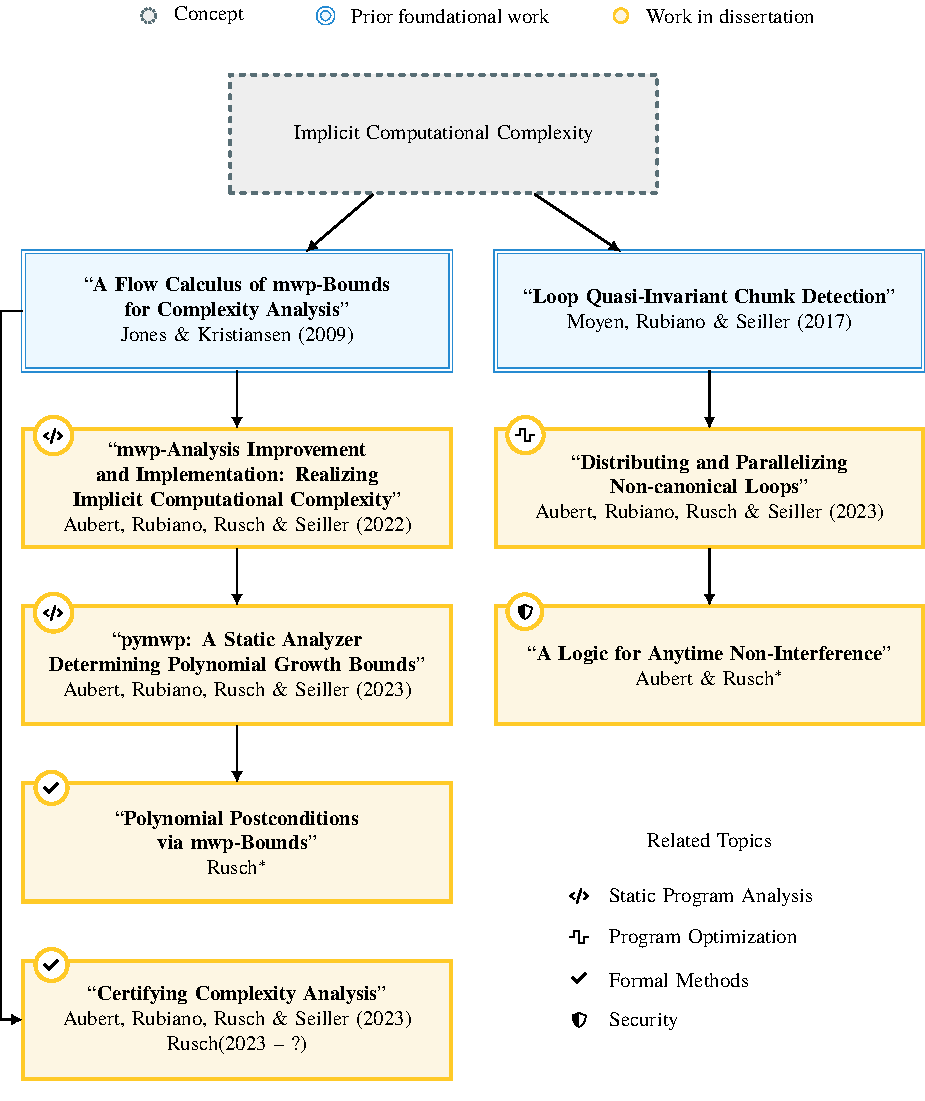
\includegraphics[width=\linewidth,keepaspectratio]{fig_conn_papers}
\end{subfigure}
\begin{center}
\resizebox{.85\textwidth}{!}{
\begin{subfigure}{\textwidth}{
\begin{tabularx}{\textwidth}{@{}X@{}cr@{}}
\toprule
\textbf{Title} & \textbf{Section} & \textbf{Background} \\
\midrule
{mwp-Analysis Improvement and Implementation\ldots}
& \aref{sec:fscd}
& \ref{icc}, \ref{static-analysis}, \ref{flow-calculus} \\
{Distributing and Parallelizing Non-canonical Loops}
& \ref{sec:vmcai}
& \ref{transforms} \\
{Polynomial Postconditions via mwp-Bounds}
& \ref{sec:postcond}
& \ref{flow-calculus}, \ref{verification} \\
{pymwp: A Static Analyzer Determining\ldots}
& \ref{sec:atva}, \aref{app:toolguide}
& \ref{icc}, \ref{static-analysis}, \ref{flow-calculus} \\
{A Logic for Anytime Non-Interference}
& \ref{sec:anytime}
& \ref{pl-sec} \\
{Certifying Complexity Analysis}
& \ref{coqpl}
& \ref{flow-calculus}, \ref{verification} \\
\bottomrule
\end{tabularx}}
\end{subfigure}}
\end{center}
\caption{Dissertation manuscripts.}
\label{fig:conn_papers}
\end{figure}

\subsection{Tips for Interacting With This Document}
\label{subsec:tips}

\subsubsection{Software Artifacts}\label{subsub:sw}
Each published and publication-ready manuscript in this dissertation, including the dissertation itself, comes with a corresponding software artifact.
A complete index of the artifacts is in~\aref{app:sec:artifacts}.
Each piece of software is archived for long-term retention, according to the long-term archival policies of the Association for Computing Machinery artifact guidelines~\cite{acm_badging}.
The software is achieved even if the venue of a manuscript did not arrange a formal artifact evaluation round.
Thus, each manuscript extends beyond the paper pages of this dissertation.

\subsubsection{Indices and Glossaries}

For convenience of the reader, this dissertation comes with three indices and glossaries\index{hello}\symbo{bigomega}.
The Term Index, in \autoref{sec:app:index}, lists technical terms and identifies where they are used in the dissertation.
The dissertation uses various acronyms where each acronym is defined at first-use.
To locate the long form afterward, refer to~\nameref{\acronymtype}.
A similar glossary is available for symbolic notations in the~\nameref{symbols}.

\subsubsection{Back-up Archival of External Documents}

The unpublished or miscellaneous external web pages and PDF files, that are referenced in the bibliography of this dissertation,
are pre-emptively archived on the Internet Archive with the Wayback Machine.
To recover a document from the Internet Archive, use the following format, substituting \pr|<URL>| by the document's URL\@.
\begin{center}
    \pr|https://web.archive.org/web/<URL>|
\end{center}
For example, the following URL may disappear in the future.
\begin{center}
    \url{https://types22.inria.fr/files/2022/06/TYPES_2022_paper_14.pdf}
\end{center}
In that case, the corresponding Internet Archive address produces the same document.
\begin{center}
    \url{https://web.archive.org/web/https://types22.inria.fr/files/2022/06/TYPES_2022_paper_14.pdf}
\end{center}

If a referenced external document was not readily available on the Internet even at the time of writing this dissertation,
the document is hosted and archived with the software deposit of this dissertation, \cf~\autoref{subsub:sw}.

\subsubsection{Line Numbers}
When referring to a specific line of source code,
we write \pr|L|, for \underline{L}ine;
followed by a natural number or numeric range that specifies the row(s) of interest.
For example, \pr|L3| means \enquote{line number 3}, and \pr|L10|--\pr|12| mean \enquote{lines 10 through 12}.


\clearpage\section{Review of the Literature}\label{sec:pre}

Literature review and discussion of the rationale of the project.
It is expected that the literature review will be more comprehensive than
those presented in the included publications.

\subsection{Literature Topic 1: Implicit Computational Complexity}\label{icc}
Theoretical computer science studies the fundamental capabilities and limitations of computation.
A function is \emph{computable}\index{computable function}
if it is algorithmically solvable in principle~\cite[p. 234]{sipser2012}.
However, computability is independent of the required computational resources\index{resource usage},
\ie \emph{cost} or \emph{resource usage} of computation.
A computable function that requires an excessive amount of resources may not be solvable in practice.

Computational complexity theory\index{complexity theory} enhances the study of computable functions\index{computable function} by classifying them into \emph{complexity classes}\index{complexity class}\footnote{
    For an archive and exploration of complexity classes, see \href{https://complexityzoo.net/Complexity_Zoo}{ComplexityZoo.net}.}
based on resources requirements\index{resource usage}.
Algorithms computing those functions are categorized by the amount of required \emph{resources}\index{resource usage} when executed on a specified \emph{machine model}, such as a Turing Machine (TM)\index{Turing Machine}.
Which particular model of computation\index{machine model} is used does not matter, as long as one adheres to Slot and van Emde Boas Invariance Thesis\index{Invariance Thesis}~\cite{slot1984}\footnote{
    The Invariance Thesis\index{Invariance Thesis} asserts that a time (resp., space) cost model is reasonable for a computational model C\index{machine model} if there are mutual simulations between TMs and C such that the overhead is polynomial in time\ccxi{p} (resp., linear in space)~\cite{vanoni2022}.},
and is concerned with complexity classes\index{complexity class}, \ie, order of magnitudes in the resources needed.
The resource cost\index{resource usage} is estimated relative to the input size.
This way algorithms are allowed to consume more resources when the input size grows while maintaining membership in the same complexity class\index{complexity class}.
The common resources of interest are time\index{time complexity} and space (memory)\index{space complexity}.
Complexity measures\index{complexity measure} are defined explicitly relative to the machine model\index{machine model}.
For example, time complexity\index{time complexity}
refers to the maximum number of computation steps a machine\index{machine model} uses on any input~\cite[p. 276]{sipser2012}.
Besides (deterministic) time and space, various other resources can be viewed as complexity measures\index{complexity measure};
for example, parallel time\index{parallel time} and circuit complexity\index{circuit complexity}~\cite[p. 428]{sipser2012}.

\emph{Asymptotic analysis}\index{asymptotic analysis} is an approach for obtaining an estimation of an algorithm's resource requirements~\cite[p. 267--277]{sipser2012}\index{resource usage}.
The analysis result is expressed as \emph{asymptotic bounds}\index{asymptotic bounds}.
The \(\mathcal{O}\)-notation\symbo{bigo} (\enquote{big-oh}) denotes an asymptotic upper bound~\cite[p. 47]{cormen2022}\index{upper bound}.
However, the bound may or may not be asymptotically tight\index{tight bound}.
The \(o\)-notation\symbo{smallo} (\enquote{small-oh}) distinguishes an upper bound that is not asymptotically tight~\cite[p. 50]{cormen2022}.
Other relevant notations are \(\Omega\)\symbo{bigomega} for an asymptotic lower bound\index{lower bound},
and \(\Theta\)\symbo{bigtheta} for an asymptotic tight bound\index{tight bound}~\cite[Sect. 3.1]{cormen2022}.
Among the benefits, complexity analysis\index{asymptotic analysis} develops insight of costs\index{resource usage} of computational patterns and identifies relationships between complexity classes\index{complexity class}.
For algorithms, it produces measures of efficiency, and allows comparing relative performance of alternative algorithms~\cite{cormen2022}.

This overview of the classical complexity theory\index{complexity theory} should be familiar from textbooks.
However, a refresher on the basics gives a baseline for comparison for the discussion that is about to follow.
The remainder of this dissertation builds on \emph{implicit} computational complexity.
Implicit complexity complements the classical complexity theory\index{complexity theory} by offering alternative perspectives and systems for reasoning about cost of computation\index{resource usage}.

\subsubsection{Computational Complexity, \emph{Implicitly}}

\emph{Implicit Computational Complexity} (ICC) is a subfield of computational complexity theory\index{complexity theory} that explores \emph{machine-free characterizations} of complexity classes\index{complexity class}.
It inherently shifts focus from computational models\index{machine model} to \emph{programs}.
\begin{quotation}
    \noindent By implicit, we here mean that classes are not given by constraining the amount of resources\index{resource usage} a machine\index{machine model} is allowed to use, but rather by imposing linguistic constraints on the way algorithms are formulated~\cite[p. 90]{dallago2011}.
\end{quotation}
In other words, complexity classes\index{complexity class} are described independently of notions of time or space related to a machine's definition.
For example, polynomial time complexity\ccxi{p} has been thoroughly examined under these terms.
The Cobham–Edmonds's Thesis~\cite{cobham1965,edmonds1965}\index{Cobham–Edmonds's Thesis} relates polynomial time class with the class of feasible functions\index{}\footnote{
    The Cobham-Edmonds Thesis asserts that the time complexities in any two \enquote{reasonable and general} models of computation are polynomially related;
    that is, a problem has time complexity \(t\) in some reasonable and general model of computation
    if and only if it has time complexity poly(\(t\)) in the model of single-tape Turing machines~\cite[p. 33]{goldreich2008}.}.
Multiple distinct implicit characterizations are known for many complexity classes\index{complexity class} -- \cf~\autoref{tab:icc-results}.

Implicit computational complexity sees complexity bounds as consequences of restrictions on program structures.
In this view, it studies the computational resources embedded in programming languages by \emph{construction}.
Another common feature is that the characterizations may omit references to explicit resource bounds~\cite{moyen2017} -- refer to \eg~%! suppress = MathFunctionText
\textcite{bellantoni1992} or~\textcite{kristiansen2005} for examples.
Thus, the focus is on studying the quality, rather than quantity, of the resources needed.
Since an implicit characterization, or an \emph{ICC system}, captures a specific complexity class\index{complexity class}, complexity analysis becomes a task of determining class membership, rather than classifying computations among many classes as in classical asymptotic analysis\index{asymptotic analysis}.

There are several good motivations for researching implicit characterizations of complexity classes\index{complexity class}~\cite[p. 36]{kristiansen2017,jones1999}, including the following.
\begin{itemize}

    \item Implicit complexity drive better understanding of complexity classes\index{complexity class} and sheds light on the notorious hard open problems of complexity theory\index{complexity theory}.

    \item From a programming language perspective, implicit complexity is motivating because it suggests ways to control complexity properties, and quantifies the computational power present in programming languages by construction.

    \item A programming language-based approach yields more {natural definitions and proofs} of central results than the classical approach.

    \item The characterizations demonstrate that complexity classes are intrinsic mathematical entities that do not depend on a particular machine model\index{machine model}.

    \item Implicit complexity introduces orthogonal program analysis techniques with potential to convert complexity-theoretic insights to practical analyses.

\end{itemize}

\subsubsection{Complexity via programming languages}

Describing the goals of implicit complexity omits the details of \emph{how} such implicit characterizations should be designed.
Over time, numerous distinct systems have been developed based on, or inspired by, \eg
calculi,
term rewriting\index{term rewriting},
data flow analysis\index{data flow analysis},
primitive recursion\index{primitive recursion},
linear logic\index{linear logic},
modal logic\index{modal logic},
type systems\index{type system},
digital circuits\index{digital circuit}, and more~\cite{kristiansen2017,marion2011,moyen2017,baillot2012}.
With such rich versatility, it becomes challenging to identify ICC systems upon encounter and to find an overarching definition that matches them all\footnote{
    On the the challenges of describing ICC systems,~\textcite[p. 14]{moyen2017} writes:
    \enquote{For a long time, I have been convinced that ICC systems are like the proverbial blind men approaching an elephant:
    each touching a different part and describing it in terms that let the others think this is a different beast.}}.

\begin{figure}[t]
    \begin{mdframed}
        \paragraph*{Implicit complexity in a nutshell.}
        The goal of implicit computational complexity can be summarized as follows.
        Let \(\mathcal{L}\)\symbo{lang} be a programming language,
        \(\mathcal{C}\)\symbo{cclass} a complexity class\index{complexity class},
        and \(\sem{p}\)\symbo{funprog} the function computed by program \(p\)\symbo{prog}.
        Then, the task is to find a restriction \(\mathcal{R}\)\symbo{restriction} \(\subseteq \mathcal{L}\), such that the following equality holds:
        \begin{align*}\{ \sem{p} \mid p \in \mathcal{R} \} = \mathcal{C}.\end{align*}
        The variables \(\mathcal{L}\),
        \(\mathcal{C}\), and
        \(\mathcal{R}\) are the parameters that vary greatly between different ICC systems.
    \end{mdframed}
    \caption[Implicit complexity in a nutshell.]
    {Description of ICC systems -- adapted from~\textcite[p. 7]{pchoux2020}}
    \label{fig:icc_systems}
\end{figure}

Recent reflective works~\cite{pchoux2020,hoffmann2022} converge on descriptions centered on programming languages.
\autoref{fig:icc_systems} summarizes the idea succinctly.
In this view, the unifying factor of implicit complexity is to find natural characterizations of complexity classes\index{complexity class} through \emph{restrictions} embedded in \emph{programming languages}~\cite{hoffmann2022}.
It requires introducing a language-based \emph{syntactic} restriction that guarantees a \emph{semantic} property;
typically, that a satisfactory program is a member of the characterized complexity class~\cite{moyen2017}\index{complexity class}.
Then, if the restriction is maintained, the complexity bound will also be maintained.

The programming language-based approach has minimally two significant effects compared to classical complexity theory\index{complexity theory}.
The first is a \emph{temporal} shift that arises from making complexity an \emph{apriori} consideration in the language design.
In other words, implicit complexity systems permit reasoning about runtime properties \emph{before a program exists}.
The second is a \emph{relational} shift between a program developer and the task of performing complexity analysis\index{asymptotic analysis}.
By embedding into a language a restriction by which a complexity bound will be guaranteed, the effort of satisfying that restriction is raised upstream to the developer~\cite{moyen2017}.
In return, to obtain runtime guarantees, the developer does not need to know about the intricacies of complexity analysis or classes.
The developer can focus on writing programs and the program's behavioral guarantees are obtained for free.
Of course, this assumes that the restriction is not excessively prohibitive in expressing algorithms.

\subsubsection{Implicit complexity by example: {safe recursion}}
\label{safe-rec}\index{safe recursion}

This example is adapted from a presentation by Dal Lago~\cite{dallago2022}.
Consider Kleene's algebra\index{Kleene algebra} of general recursive functions\index{recursive function} as a programming language.
In this language, programs are built from basic building blocks (the initial functions) by %way of
composition, primitive recursion\index{primitive recursion}, and minimization.
%Dropping minimization makes this formalism strictly less expressive: the functions one represents (the so-called primitive recursive functions) are, at least, all total.
Primitive recursive functions\index{recursive function} are
%however
well beyond any reasonable complexity class\index{complexity class}
%They are after all the class of functions which can be computed in time and space bounded by primitive recursive functions, the latter being strictly larger than Kalmar's elementary functions. %Essentially, this is
due to the possibility of having nested recursive definitions.
As an example, one can define addition from the initial functions

\begin{center}
\(\text{add}(0, x) = x\);

\(\text{add}(n + 1, x) = \text{add}(n, x) + 1\);
\end{center}

and then define exponentiation \(n \mapsto 2^n\) from addition as follows:

\begin{center}
\(\text{exp}(0) = 1\);

\(\text{exp}(n + 1) = \text{add}(\text{exp}(n), \text{exp}(n))\).
\end{center}

\noindent Composing exp with itself allows us to form towers of exponentials of arbitrary size. %, thus saturating the Kalmar elementary functions.
A recursion on exp leads us even beyond the class of elementary recursive functions\index{recursive function}; %aforementioned class,
already too broad complexity-wise.

Rather than removing primitive recursion\index{primitive recursion} from the algebra up-front (which would have too strong an impact on the expressive power), % of the underlying function algebra)
we want to refine the algebra by distinguishing arguments that matter for complexity from arguments that do not.
The arguments of any function \(f\)\symbo{f} are dubbed either as \emph{normal}, when their value can have a relatively big impact on \(f\text{'s}\)\symbo{f} complexity, or \emph{safe} when their value can only influence \(f\)\(\text{'s}\)\symbo{f} behavior very mildly. %, combinatorially speaking.
If \(\vec{x}\)\symbo{normx} are the normal parameters and \(\vec{y}\)\symbo{safey} are the safe ones,
we indicate the value of \(f\)\symbo{f} on \(\vec{x}\)\symbo{normx} and \(\vec{y}\)\symbo{safey} as \(f(\vec{x};\vec{y})\)\symbo{normx}\symbo{safey},
where the semicolon separates the normal from the safe.
This way, the usual scheme of primitive recursion\index{primitive recursion} can be restricted as follows:

\begin{center}
    \(f (0, \vec{x};\vec{y}) = h (\vec{x};\vec{y})\);

    \(f (n + 1,\vec{x};{ }\vec{y}) = g (n, \vec{x}; \vec{y}, f(n,\vec{x}; \vec{y})) \).
\end{center}

%Please notice that
\noindent The way we define \(f\)\symbo{f} from \(g\) and \(h\) is morphologically identical to what happens in the usual primitive recursive scheme.
That it is a restriction is a consequence of the distinction between normal and safe arguments: the recursive call \(f(n,\vec{x}; \vec{y})\)\symbo{normx}\symbo{safey} is required to be forwarded to one of g's safe argument, while the first parameter of \(f\)\symbo{f} must be normal.
This makes exp not expressible anymore, giving rise to new function algebra called \emph{safe recursion}\index{safe recursion}, discovered by Bellantoni and Cook~\cite{bellantoni1992} (BC in the following).

\begin{theorem}
    The class BC equals the class FP of polynomial time computable functions.
\end{theorem}\ccxi{p}

\subsubsection{A snapshot of theoretical results}
\label{icc-theories}

The breakthrough result of safe recursion\index{safe recursion} is regarded as the first implicit characterization of a complexity class\index{complexity class}~\cite{dallago2011,kristiansen2017,rubiano17}.
However, the same result was independently discovered by~\textcite{leivant1993} in a slightly different setting of stratified recurrence\index{stratified recurrence}~\cite[p. 762]{dallago2022}.
\autoref{tab:icc-results} shows a {very small} collection of additional impactful theoretical results.
The inclusion criteria is varied and based on representing the rich variety of underlying techniques or complexity classes\index{complexity class};
or for presenting foundational techniques that have been extended later;
or for reflecting shifts in theoretical developments and interests over time.
The table also marks with hyperlinks works that are discussed elsewhere in this dissertation.
These theoretical results provide a conceptual \enquote{toolbox} of techniques that form the foundation
for the rest of this dissertation.

%! suppress = LineBreak
%! suppress = NonBreakingSpace
\begin{tabularx}{\textwidth}{@{}lclXr@{}}
    \multicolumn{5}{@{}c@{}}{\resizebox{\textwidth}{!}{
        \textbf{Symbols.}
        \hspace{.6em}\logics{ }logics
        \hspace{.6em}\types{ }type system
        \hspace{.6em}\dataflow{ }data flow
        \hspace{.6em}\syntax{ }syntactic
        \hspace{.6em}\lalg{ }algebras
        \hspace{.6em}\recs{ }recursion}} \\*[1em]
    \toprule
    \textbf{Year} & &
    \textbf{Venue} &
    \multicolumn{2}{l@{}}{\textbf{Description}\hfill\textbf{Complexity Classes}}
    \\
    \midrule
    \endfirsthead
    \multicolumn{5}{@{}c@{}}{\resizebox{\textwidth}{!}{
        \textbf{Symbols.}
        \hspace{.6em}\logics{ }logics
        \hspace{.6em}\types{ }type system
        \hspace{.6em}\dataflow{ }data flow
        \hspace{.6em}\syntax{ }syntactic
        \hspace{.6em}\lalg{ }algebras
        \hspace{.6em}\recs{ }recursion}} \\*[1em]
    \toprule
    \textbf{Year} & &
    \textbf{Venue} &
    \multicolumn{2}{l@{}}{\textbf{Description}\hfill\textbf{Complexity Classes}}
    \\
    \midrule\endhead
    \caption[]{(Cont.)}
    \endfoot
    \endlastfoot
    1992\(^*\) & \syntax & Comput  & Safe recursion\index{safe recursion} -- \autoref{safe-rec} & \ccx{p} \\*
    && Complex. & \textcite{bellantoni1992} \\*
    \midrule
    1993\(^*\) & \recs & POPL & Stratified recurrence\index{stratified recurrence} & \ccx{p} \\
    &&& \textcite{leivant1993} \\*
    \midrule
    1995 & \lalg & CSL & Tiering \aka ramification\index{tiering}\index{ramification} & \ccx{pspace} \\*
    &&& \textcite{leivant1995} \\*
    \midrule
    1999 & \types & LICS & Non-size-increasing programs\index{non-size-increasing programs} & \ccx{p} \\*
    &&& \textcite{hofmann1999} \\*
    \midrule
    2000 & \recs & LPAR & Quasi-interpretations\index{quasi-interpretation} & \ccx{p} \\*
    &&& \textcite{marion2000} \\*
    \midrule
    2001 & \syntax & J. Funct. & CONS-free programs\index{CONS-free programs} & \ccx{p}, \ccx{exp} \\*
    && Program. & \textcite{jones2001} & \\*
    \midrule
    2001 & \dataflow & POPL & Size-change termination principle\index{size-change termination principle} & \ccx{pspace} \\*
    &&& \textcite{lee2001} \\*
    \midrule
    2005 & \lalg & Comput. & \textsc{loop}\(^{-}\) and \textsc{clip} programs & \ccx{l}, \ccx{linspace} \\*
    && Complex. & \textcite{kristiansen2005} \\*
    \midrule
    2009 & \logics & TOCL & Flow calculus of mwp-bounds\index{mwp-calculus} -- \autoref{flow-calculus} & \ccx{p} \\*
    &&& \textcite{jones2009}  \\*
    \midrule
    2011 & \types & LICS & SAFE programs\index{SAFE programs} -- \autoref{icc-sec} & \ccx{p} \\*
    &&& \textcite{marion2011} \\*
    \midrule
    2013 & \types & ICALP & Ramified programs\index{ramification}\index{ramified programs} -- \autoref{icc-sec}  & \ccx{p}, \ccx{l} \\*
    &&& \textcite{leivant2013} \\*
    \midrule
    2013 & \types & & SAFE processes\index{SAFE programs!process} -- \autoref{icc-sec} & \ccx{p} \\*
    &&& \textcite{hainry2013} \\*
    \midrule
    2015 & \types & LPAR & d\(\ell\)T\index{d\(\ell\)T} programs\(^a\) -- \autoref{icc-sec} & \ccx{p} \\*
    &&& \textcite{baillot2015} \\*
    \midrule
    2016 & \logics & Inf. & Complexity with pointer machines & \ccx{l} \\*
    &&  Comput. & \textcite{aubert2016}  \\*
    \midrule
    2016 & \recs & Inf. & Complexity of uniform boolean circuits & \ccx{nc} \\*
    && Comput. &\textcite{bonfante2016} \\*
    \midrule
    2018 & \types & Inf & Object Oriented programs\index{SAFE programs!object-oriented} -- \autoref{icc-sec} & \ccx{p} \\*
    && Comput. & \textcite{hainry2018} \\*
    \midrule
    2021 & \lalg & MFCS & Probabilistic characterization \(\text{ST}_\text{PP}\) & \ccx{pp} \\*
    &&& \textcite{dallago2021} \\*
    \midrule
    2023 & \types & POPL & Stratified (STR) programs\index{stratified programs} -- \autoref{icc-sec} & \ccx{p} \\*
    &&& \textcite{hainry2023} \\*
    \midrule
    2024 & \types & POPL & Quantitative type theory\index{quantitative type theory} & \ccx{p}, \ccx{np}, \ccx{bpp} \\*
    &&& with dependent types\index{dependent types}, \textcite{atkey2024} \\*
    \midrule
    2024 & \types & LICS & Aperiodic programs\index{aperiodic programs} -- \autoref{icc-sec} & \ccx{p} \\*
    &&& \textcite{hainry2024} \\*
    \bottomrule
    \multicolumn{5}{@{}l}{\(^a\) The system can handle sub-computations not in \ccx{p}.} \\
    \caption[Theoretical implicit computational complexity systems and results.]{
        A list of theoretical implicit computational complexity systems and results.
        The historical first publications are marked with \(^*\)-symbol.
        The graphical symbols on left describe the restriction techniques for enforcing complexity bounds (limited to one symbol).}
    \label{tab:icc-results}
\end{tabularx}

\subsection{Literature Topic 2: Static Resource Analysis}\label{static-analysis}
%! suppress = LabelConvention
Asymptotic analysis, that classifies programs based on resource requirements, is the natural dual of studying complexity classes.
Since implicit computational complexity focuses on language-based characterizations, it produces analysis techniques for free.
It is a foundational hypothesis of this dissertation that theoretical ICC systems---with sufficient expressive power and an efficient evaluation strategy---enable concrete program analysis.
An analysis designed to evaluate a program's resource usage is called resource analysis.
Resource analysis is a subfield of static program analysis.

\subsubsection{Foundations of Static Program Analysis}\label{static-analysis-basics}

Static program analysis aims to answer questions about the runtime behaviors of programs.
The term \emph{static} means the analysis is conducted at compile-time on the program syntax and without execution.
The main motivations is to improve the performance characteristics of the generated executable~\cite{nielson2010,kennedy2001},
including detecting logical issues in the specification of the input program.
Foundational techniques include, \eg
type and effect systems;
control- and data-flow analyses;
abstract interpretation;
constraint-based, pointer, and inter-procedural analyses;
and fixed point algorithms~\cite{nielson2010,moller2023}.
Static program analysis is strongly practice-oriented and frequently materialized in automatic analyzers.
Real-world software development tools---like compilers, interactive development environments, and verifiers---rely on static analyses~\cite{livshits2015}.
A core challenges of static analysis concern precision and scalability of the techniques;
these topics are actively explored in research~\cite{schiebel2024}.

As a consequence of Rice's theorem~\cite{rice1953}\footnote{
Informally, Rice's theorem asserts that all interesting questions about the input/output behavior of programs written in a Turing-complete language are undecidable.}, it is impossible to construct a perfect program analyzer for a Turing-complete language.
All approaches must sacrifice something among soundness, completeness and termination~\cite{moller2024}.
Although seemingly discouraging, Rice's theorem should be viewed with optimism.
Since static program analysis is inherently undecidable, there is infinite opportunity in building increasingly precise approximations --
for inspiration see, \eg~\textcite{ding2023}.
The challenge is then to design analysis techniques that produce \emph{useful} answers \emph{efficiently} and \emph{often enough}.
This is colloquially called the \enquote{full employment theorem for static program analysis designers}~\cite[p. 4]{moller2023}.

Static analyzers typically evaluate programs against semantic properties\footnote{
Properties are introduced in~\autoref{verification-concepts}, but previewed here briefly.}.
More specifically, the focus is on \emph{safety properties}~\cite[p. 6]{moller2023},
which assert that something bad will not happen~\cite{lamport1977}.
Examples of safety properties include memory safety, absence of overflows, termination, and secure information flow (\cf~\autoref{if-elements}).
Safety properties have many applications in bug finding, program optimization, verification, \etc

\subsubsection{The Challenge of Approximation}\label{static-approx}

There are two broad categories of static analyzers~\cite{jourdan2015}.

\begin{itemize}

\item A \emph{bug finder} must discover potential errors that are hard to find by testing.
The analysis must be precise because excessive false alarms make the tool unusable.
The \emph{precision}\index{precision} of an analysis is the degree to which it avoids erroneous results~\cite{livshits2015}.
However, a bug finder offers no guarantee that all bugs will be found.

\item A program \emph{verifier} must establish that a given safety property holds with high confidence.
Critically, the analyzer must account for all execution paths.
If the analyzer reports no alarms, then it must be the case that the program is free of the errors tracked by the analyzer.

\end{itemize}

Obtaining the intended behavior depends on design choices, particularly on how the analysis approaches soundness and completeness.

\begin{figure}[t]
\centering
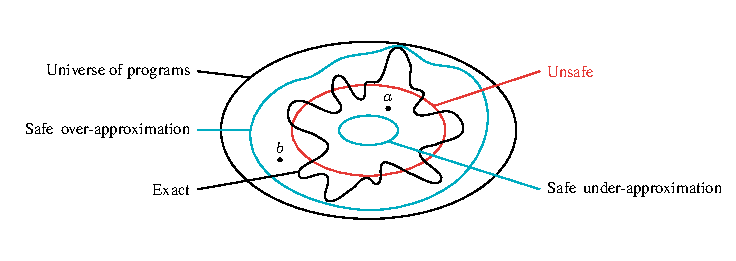
\includegraphics[width=\textwidth,keepaspectratio]{fig_approx}
\caption[Program analysis as an approximation.]{
Program analysis as an approximation -- an illustration inspired by~\textcite{steffen2020}.
The \textsc{exact} class of programs satisfying the analyzed property \(\phi\) is undecidable.
The program \(a\) satisfies \(\phi\), but the program \(b\) does not.
For an analyzer making a \textsc{safe under-approximation}, every accepted program truly satisfies \(\phi\), but would give an erroneous result on \(a\).
An analyzer making a \textsc{safe over-approximation} would accept \(a\) and \(b\), even though \(b\) does not satisfy \(\phi\).
However, an over-approximating analyzer never misses programs that satisfy \(\phi\).
Although an \textsc{unsafe} analysis can be justifiable in some cases,
interpreting its results is problematic because errors are not conservative.
}\label{fig:approx}
\end{figure}

\paragraph*{Soundness and completeness.}
A terminating static analyzer can either be sound or complete, but not both.
Soundness and completeness are terms from logic and not exclusive to static program analysis.
In logic, they carry the following meaning.
\begin{itemize}
\item A \emph{sound}\index{soundness} system guarantees that everything that is provable is true.
\item A \emph{complete}\index{completeness} system guarantees that everything that is true has a proof.
\end{itemize}
In the context of program analysis,
if a provably sound system reports that some property holds, then it must be true for the analyzed program.
A sound analyzer never misses a violation---\ie when a property does \underline{not} hold---but it may report an erroneous result for a satisfactory program~\cite{torlak2015}.
A complete analyzer detects all satisfactory programs, but also accepts cases where the tracked property does not truly hold.
The analysis approximation should be \emph{conservative}\index{conservative analysis}
whereby all errors occur on the \enquote{safe side} of the application domain~\cite[p. 5]{moller2023}.
Refer to Figures~\ref{fig:approx} and~\ref{fig:bug-verify} for examples.

\begin{figure}[t]
\centering
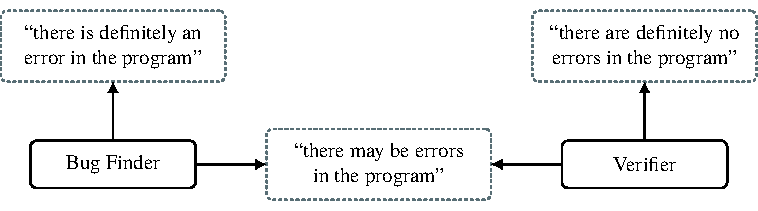
\includegraphics[width=.85\textwidth,keepaspectratio]{fig_bug-verifier}
\caption[Sound and incomplete bug detector vs. verifier]{
Behavior of sound and incomplete static analyzers: bug detector vs. verifier~\cite{moller2024}.
An \enquote{error} refers to some property tracked by the analyzer.}
\label{fig:bug-verify}
\end{figure}

To offer guarantees, a sound analyzer must overestimate the program behaviors.
It models all execution paths, including those that do not occur in any execution, like all branches of a conditional statement.
Soundness is challenging because it can render the analysis unscalable or imprecise to the point of being useless.
To maintain semantics, an optimizing analysis typically requires soundness~\cite[p. 5]{moller2023}.
A complete analyzer underestimates the program behaviors and thus errs on the other side.

\paragraph*{Soundiness.}
While academic literature widely emphasizes sound analyses, according to~\textcite{livshits2015}, strict soundness is a myth among realistic whole-program analyzers.
Practically-orientated static analyzers typically insist on Turing-completeness and termination,
but trade between soundness and completeness~\cite{moller2023,steffen2020}.
As an compromise, modern analyzers for real programming languages are often soundy.
A \emph{soundy}\index{soundy} analysis is as sound as possible, without excessively compromising precision or scalability~\cite{livshits2015}.

\subsubsection{Techniques of Resource Analysis}\label{resource-analysis}

Resource analysis\index{resource analysis}\footnote{
Also called \emph{cost analysis} when using an explicit \emph{cost measure}\index{cost measure}~\cite{albert2008}.
}---or (static/automatic) {complexity analysis}~\cite{rosendahl1989,leivant2013}---%
aims to obtain static information about the runtime {execution cost}\index{execution cost} of an analyzed program.
Such analysis naturally decomposes into two parts: one concerning the program's execution time and termination;
and the other change in the program's data-size~\cite{jones2009}.
Numerous techniques can be used to reason about such properties.

\begin{itemize}
\item Termination analyses tend to focus on values that are copied or decreased.
      Establishing termination is a critical aspect of correctness of recursive calls and commands.
      Termination analyses aim to discover conditions---like difference constraints~\cite{sinn2017},
      program-dependent well-founded orders on loops~\cite{lee2001}, or
      establishing that recursive reduction sequence are finite\footnote{
      Showing that every reduction sequence is finite is called the \emph{strong normalization} property~\cite[p. 36]{bertot2004}}---
      that guarantee termination.
      A specific technique for termination analysis, that originates from implicit computational complexity, is the size-change termination principle\index{size-change termination principle} of~\textcite{lee2001}.
\item Data-size analyses focus on memory consumption, estimating how large various variable values may become~\cite{lommen2023}.
      Obtaining bounds thus requires studying patterns of data-size changes during computation.
      In imperative programs, interesting data-size behaviors arise from counter increments and resets, particularly in loops~\cite{sinn2017,benamram2020}.
\end{itemize}

This dissertation is concerned with techniques of data-size analysis.
Among the specific and well-established techniques are automatic amortized resource analysis and cost equation systems, presented briefly next.

\paragraph*{Automatic amortized resource analysis.}
Amortized analysis\index{amortization} averages the time required to perform a sequence of operations over all the operations performed~\cite[p. 451]{cormen2009}.
It enables to show that the average cost of an operation is small, even if a single operation might be expensive.
Automatic amortized resource analysis (AARA)~\cite{hoffmann2022} builds on this idea to provide an automatic static technique for deriving arithmetic resource bounds.
AARA bounds programs based amortized analysis, which adds the ability to account for amortization effects across operation sequences.
The analysis relies on inference rules, and derivation trees provide proofs of the resource bounds.
AARA originated from works in implicit computation complexity, particular from the contributions of Martin Hofmann~\cite{hoffmann2022}.
AARA-based techniques has been implemented on functional~\cite{hoffmann2017}, imperative~\cite{carbonneaux2015,carbonneaux2017}, and probabilistic~\cite{ngo2018} programming languages.

\paragraph*{Cost equation systems.}
A \emph{cost equation system} (CES) (alternatively: cost relation system) is an abstract representation format of a program's resource cost~\cite{floresmontoya2017,albert2019}.
It consists of a set of cost equations, that are non-deterministic recurrence relations annotated with constraints, as shown in \autoref{lst:ces}~\cite{floresmontoya2014}.
The analyzing technique of cost equations is based on the seminal work of~\textcite{wegbreit1975}.
Such analysis operates in two phases.
The first phase extracts a set of equations that capture the program cost \wrt data-size and a parametric cost measure.
%\footnote{The generation phase converts the program's iteration constructs (loops and recursion) into recurrences,
%then infers size relations that approximate how the program's argument sizes vary.}.
This set can be regarded as recurrence relations, or as a kind of time-bound programs of~\textcite{rosendahl1989}.
The second phase searches for a non-recursive representation of the equations known as \emph{closed form}.
In most cases, it is not possible to find an exact solution, and the closed form provides an upper bound~\cite{albert2008}.
Cost equations deal with loops and recursion in a uniform manner,
but may have issues with multiphase loops and with programs with require complex termination proofs~\cite{floresmontoya2014}.

\begin{center}
\begin{minipage}{\textwidth}
\captionsetup{type=lstlisting}
\cesinputlisting{example.ces}
\captionof{lstlisting}[A cost equation system]{
A cost equation system representing an exponential function.
The term \pr|a(n)| is called the {head} and the rightward terms are the {body}.
The body terms represent costs and constraints.}
\label{lst:ces}
\end{minipage}
\end{center}

\subsubsection{A Sampler of Public Static Resource Analyzers}
\label{resource-analysis-tools}

The following list presents a small survey of automatic complexity analysis implementations, interpreted broadly.
It prioritizes tools that are open source or, at minimum, provide a public interface.
A comprehensive comparison of resource bounds computed by various tools is available online~\cite{flores_experiments}.

\begin{description}

\item[\href{https://costa.fdi.ucm.es/~costa/pubs/pubs.php}{{PUBS}}]
      \emph{\underline{P}ractical \underline{U}pper \underline{B}ounds} \underline{S}olver~\cite{albert2010}\index{PUBS}
      is a CES solver that computes closed form upper bounds for cost equation systems\index{cost equation system};
      specifically, for the \pr|entry| and all cost equations that depend on \pr|entry|.

\item[\href{https://aprove.informatik.rwth-aachen.de}{{AProVE}}]
      \emph{\underline{A}utomated \underline{Pro}gram \underline{V}erification \underline{E}nvironment}~\cite{giesl2017}\index{AProVE}
      produces termination proofs and complexity bounds for
      term rewrite systems,\index{term rewrite system},
      Java bytecode\index{bytecode},
      and programs written in
      C\index{C},
      Prolog\index{Prolog}, or
      Haskell\index{Haskell}.
      AProVE is a regular contestant in international tool competitions, including the
      \href{https://termination-portal.org/wiki/Termination_Competition}{Termination Competition}~\cite{giesl2019}
      and \href{https://sv-comp.sosy-lab.org/}{Competition on Software Verification} (SV-Comp)~\cite{beyer2022}.

\item[\href{https://github.com/aeflores/CoFloCo}{{CoFloCo}}]
      \emph{\underline{Co}ntrol \underline{Flo}w refinement of \underline{Co}st Relations}~\cite{floresmontoya2014}\index{CoFloCo}
      is an open-source analyzer and CES solver that infers symbolic upper and lower complexity bounds for CESs.
      CoFloCo is not bound to any particular programming language, but expects a input program translated to a CES\@.

\item[\href{https://github.com/academic-archive/pldi15}{C4B}]\cite{carbonneaux2015}\index{C4B}
      is an AARA-based analyzer of certified compositional resource bounds.
      It infers linear resource bounds on C-like programs by amortization\index{amortization} -- \autoref{tab:atva-compare}.

\item[\href{http://cl-informatik.uibk.ac.at/software/tct/}{TcT}]
       \emph{\underline{T}yrolean \underline{C}omplexity \underline{T}ool}~\cite{avanzini2016}\index{TcT}
       is a modular analyzer with front-ends to support term rewrite- and integer transition systems;
       high-order functional programs, and Java bytecode.
       The complexity problem and metric of interest are parametric.
       TcT has also competed in the Termination Competition.

\item[\href{https://koat.verify.rwth-aachen.de/cfr_mprf}{KoAT}]
       \emph{\underline{Ko}mplexitäts-\underline{A}nalyse-\underline{T}ool}~\cite{brockschmidt2016}\index{KoAT}
       is a complexity analyzer for computing time-, cost- and size bounds.
       As inputs, KoAT accepts Integer Programs (IPs)\index{integer program} and C integers programs that follow
       \href{https://termination-portal.org/wiki/C_Integer_Programs}{the grammar specification} of the Termination Competition -- \autoref{pc-expr}.

\item[\href{https://github.com/statycc/LQICM_On_C_Toy_Parser}{LQICM}]
      \emph{\underline{L}oop \underline{Q}uasi-\underline{I}nvariant \underline{C}hunk \underline{M}otion}~\cite{moyen20172}\index{LQICM}
       is a compile-time program optimization pass for C programs.
       It aims to peel (\cf~\autoref{loop-transforms}) inner loops to reduce program's time complexity.

\item[\href{https://www.raml.co/about}{RaML}]
       \emph{\underline{R}esource \underline{a}ware \underline{ML}}~\cite{hoffmann2017}\index{RaML}
       is an analyzer of worst-case upper bounds and best-case lower bounds of cost, for functional programs written in OCaml\index{OCaml}.
       The cost resource can be any quantity that is of interest.
       The RaML analysis is based on AARA and can produce precise amortized bounds.

\item[\href{https://github.com/academic-archive/cav17-pastis}{Pastis}]\cite{carbonneaux2017,carbonneaux2018}
      is an AARA-based analyzer.
      It infers various resource bounds and size change information of programs expressed in LLVM bitcode (interprocedural CFGs).
      Additionally, it generates proof certificates that guarantee the validity of the inferred bounds.

\item[\href{http://cl-informatik.uibk.ac.at/users/zini/software/hosa/}{HoSA}]
      \emph{\underline{H}igher-\underline{O}rder \underline{S}ize \underline{A}nalysis}~\cite{avanzini2017}\index{HoSA}
      is a time complexity analyzer for higher-order functional programs written in a (generic) strongly typed functional programming language.
      The analysis technique is based on a type system and inference of sized types, and constraint solving.

\item[\href{https://github.com/davidnowak/cecoa}{Cecoa}]\cite{feree2018}\index{Cecoa}
     is a formal methods library based on implicit computational complexity.
     It enables creating proofs to show a program is poly-time computable\ccxi{p} -- \autoref{icc-formally}.

\item[\href{https://costa.fdi.ucm.es/maxcore/}{MaxCore}]%
      \emph{\underline{Max}-SMT termination analyzer + \underline{CO}st \underline{R}ecurrence \underline{E}quation solver}~\cite{albert2019}\index{MaxCore}
      is an upper bounds complexity analyzer for C programs\index{C}.
      The underlying technique is based on cost equations and termination analysis, and MaxCore uses CoFloCo and PUBS as back-end CES solvers.

\item[\href{https://www-sop.inria.fr/members/Martin.Avanzini/software/eco-imp/}{eco-imp}]\cite{avanzini2020}\index{eco-imp}
      computes expected cost bounds for programs written in a probabilistic imperative \textsc{pWhile} language.

\item[\href{https://gitlab.inria.fr/complexityparser/complexityparser}{ComplexityParser}]\cite{hainry2021}\index{ComplexityParser}
      is a complexity analyzer for Java\index{Java} programs.
      A typable program is guaranteed to run in polynomial time if the program terminates.
      The analyzer is based on~\cite{hainry2015} and~\cite{hainry2018}, discussed more in~\autoref{icc-sec}.

\item[\href{https://github.com/statycc/pymwp}{pymwp}]\cite{aubert2023b}\index{pymwp}
      is an implementation of the flow calculus of mwp-bounds.
      It is purely syntactical analysis of C\index{C} programs, to determine if the program's variable value growth is polynomially bounded in inputs -- \autoref{sec:atva}.

\item[\href{https://zenodo.org/records/10457566}{Quantitative probabilistic bounds}]\cite{chatterjee2024}
      analyzer computes tail and expectation bounds for programs written
      in a probabilistic imperative programming language \textsc{Prog}.

\end{description}

\subsubsection{Feature Considerations of ICC Techniques}\label{icc-feat}

\paragraph*{Soundness and completeness.}
In characterizing a complexity class,
a \emph{soundness} statement says that all programs of a given language, or those satisfying a restriction \(\mathcal{R}\), admit a certain complexity property, \ie compute functions in the target class.
A \emph{completeness} statement says that all functions of the corresponding functional complexity class can be programmed in this language~\cite{baillot2012}.
Alternatively, if \(\mathcal{R}\) is \emph{(extensionally) complete}, then for any problem in the complexity class, there exists a program in \(\mathcal{R}\) that decides it.
For instance, for polynomial time complexity, the soundness statement refers to a polynomial time evaluation of programs, whereas completeness refers to the class FP of functions computable in polynomial time~\cite{baillot2012}.
However, extensional completeness is of limited interest, as the goal is to validate as many interesting programs as possible.

ICC systems are typically proven sound \wrt the complexity class they characterize, whereby they are \emph{sound and incomplete} under-approximations of the target class~\cite[p. 125]{moyen2017}.
A sound and incomplete analysis admits false negatives, but guarantees the absence of false positives.
Complexity analysis can then give an erroneous result in the following way:
a developer writes a program that belongs to the intended complexity class,
but the program fails the analysis because it is not expressible in the ICC system.
Fixing the issue requires rewriting the program to satisfy the class membership restriction \(\mathcal{R}\).
Due to undecidability, it is impossible to completely avoid false negatives.
Stated differently, implicit complexity can decide non-trivial semantics properties of programs, but it will always exclude some programs that possess the property of interest.

\paragraph*{Input languages and expressive power.}
Extensional correspondence with complexity classes is usually not enough.
A programming language offering safety guarantees is plausible only
if it captures enough interesting and natural algorithms~\cite{baillot2012}.
On the other hand, sacrificing Turing-completeness allows developing an analysis that is \enquote{completely correct} about membership in a particular complexity class.
It requires defining a non-Turing-complete programming language and proving that it is sound and complete \wrt a particular complexity class.
%i.e., that their programs compute functions in \(\mathbb{C}\),
%and that for any problem in \(\mathbb{C}\), there is a program that solves it).
This sidesteps Rice's theorem, but cannot be \emph{intentionally} complete, since it will always exclude programs that yet belong to the targeted complexity class.
Correctly analysing a real world programming language is very difficult because of the large number of constructions allowed in it.

\begin{quotation}
\noindent We must understand all the difficulty because for a Turing-complete language for example the class of PTime programs is not recursively enumerable, and therefore an intentionally complete criterion would not be decidable~\cite[Sect. 4.1]{mogbil2012}.
\end{quotation}

\noindent For this reason, most research\footnote{
Among exceptions, quasi-interpretations~\cite{marion2000} considers a Turing-complete language.}
in implicit complexity techniques focuses on \enquote{toy languages}~\cite{moyen2017,rubiano17};
like term rewrite systems or the \textsc{Loop} language~\cite{kristiansen2005}.
% functional, imperative (oop, loops), flowchart, term rewriting,...
While such languages capture the core of mainstream programming languages, they are far from the rich constructs allowed in real languages.
%That limits the spread of implicit complexity-based techniques beyond academic circles and complicates rigorously assessing their potential.

\paragraph*{Analysis mechanics and obtained bounds.}
That ICC systems are designed to characterize a specific complexity classes has implications on the results they produce.
If they generate bounds, they are asymptotic (symbolic) bounds, rather than concrete bounds~\cite{baillot2019}.
An existing research direction in ICC concerns improving precision of obtained resource bounds~\cite{benamram2020}.
However, if the system is designed as a sound under-approximation, it can only provide upper bounds~\cite[p. 119]{moyen2017}.
A satisfactory program can be provided run-time complexity guarantee, but nothing is known of the runtime behavior of unsatisfactory programs.
ICC system is inherently restricted to analyzing programs whose sub-computations also satisfy the membership criterion of the target complexity class~\cite{baillot2019}.
On the other hand, unlike many other static analysis techniques,
ICC systems may not require establishing termination and avoid difficult control-flow analysis by abstraction and over-approximation~\cite{jones2009}.

\subsubsection{Prospects and Directions in ICC-Based Program Analysis}

There are two general strategies for implementing static analyses based on implicit computational complexity.
The first involves restricting the program syntax to guarantee all valid programs satisfy a desired property.
This is challenging for a software engineer since it may require writing programs in an unnatural way (though not all programs are written by humans).
However, if the program can be expressed in the given syntax, then the desired property is obtained \emph{for free}.

The second strategy allows a software engineer to write any program and performs program analysis \emph{aposteriori}.
Instead of requiring every program to be written using the restriction \(\mathcal{R}\),
we would test the adhesion of the program to the restriction \(\mathcal{R}\).
While this is more preferable for the program creator, such analysis is necessarily incomplete.
Some programs will be decided incorrectly and must be refactored to be acceptable to an analyzer.
Nonetheless, this strategy already has produced applications in~\textcite{moyen2016,moyen20172}.

%But implicit computational complexity is flexible enough to extend beyond complexity properties.
%Therefore, it can be leveraged in analysis of \emph{other} semantic properties.
%For example, it is possible to use ICC systems to develop static analysis tools.

Those research lines illustrates a shift from the design of ICC programming languages -- from pre-bounding all programs --
to the design of \emph{criteria} that may or may not be met by programs written in a Turing-complete programming language.
The first observation is crucial, considering that software engineers in general focus on much more tangible functional properties,
than complexity classes.
The second observation sends a mixed signal.
It seems that ICC will lose the originality of its approach by accepting to act as a post-filter on Turing-complete programming languages.
Let us not forget that by restricting the programming language itself, ICC offers the possibility of never having to run any analysis.

Compelling related examples of systems that provide properties by construction already exist.
The safe subset of the programming language Rust guarantees \eg memory safety and deadlock freedom by design.
Strongly normalizing interactive theorem provers require \emph{structural} fixed point termination~\cite{bertot2004}.
In return, every valid programs is known to terminate.
Although a software engineer cannot write every program, if they accept the restriction, they receive the termination guarantee for free.
Conceivably, implicit computational complexity techniques can provide similar \emph{X-by-Construction}\index{X-by-Construction}~\cite{terbeek2018} guarantees.


\subsection{Literature Topic 3: The Flow Calculus of mwp-Bounds}\label{flow-calculus}
The \emph{flow calculus of mwp-bounds}\index{mwp-calculus}, introduced by~\textcite{jones2009},
is a sound and compositional complexity analysis\index{complexity analysis} technique
for reasoning about variable value growth in imperative programs\index{imperative programs}.
It tracks data-size growth in variables between commands.
The information about variable value growth is captured and expressed as \emph{mwp-bounds}\index{mwp-bound}.

More precisely, for program \pr|C|\symbo{p2} the analysis aims to discover \emph{polynomially bounded data flow relations}\index{data flow relation},
between the \emph{initial values} \(x_1,\ldots,x_n\)\symbo{xpre} of natural-number variables \(\prm{X}_1,\ldots,\prm{X}_n\)\symbo{xvar} and the \emph{final values} \(x'_i\)\symbo{xprime2} of \(\prm{X}_i\) (for \(i=1,\ldots,n\)),
that hold whenever \(\sem{\prm{C}}(x_i \rightsquigarrow x^\prime_i)\)\symbo{flowrel}.
If it is possible to determine that all variable values grow at most polynomially in inputs, the analysis assigns to program \pr|C|\symbo{p2} a \emph{bound}, \ie a conjunction of mwp-bounds\index{mwp-bound};
that characterizes the value growth of all its variables.
The conclusion is derived statically and syntactically by applying inference rules\index{inference rule} to the commands of the program.
As a motivating preview, Examples~\ref{ex:bounds1} and~\ref{ex:bounds2} demonstrate the semantic property the analysis detects.

\begin{example}[Polynomially bounded program]\label{ex:bounds1}
The variable values of the program
\begin{center}
\pr|X1=X2+X3; X1=X1+X1|
\end{center}
are bounded by \(x_1' \leq 2x_2 + 2x_3\)\symbo{xpre}\symbo{xprime2} and \(x_2' \leq x_2\)\symbo{xpre}\symbo{xprime2} and \(x_3' \leq x_3\)\symbo{xpre}\symbo{xprime2}.
Each variable can be bounded by at most a polynomial and the flow calculus\index{mwp-calculus} accepts the program.
The polynomially bounded data flow relation\index{data flow relation} \(\sem{\prm{C}}(x_1,x_2,x_3 \rightsquigarrow x^\prime_1,x^\prime_2,x^\prime_3)\)\symbo{flowrel}
holds for all variables in all program states.
\end{example}

\begin{example}[An always failing program]\label{ex:bounds2}
Consider a program that repeats, for \pr|X2|\symbo{xvar} times, an arithmetic operation on the variable \pr|X1|\symbo{xvar}.
\begin{center}
\pr|X1=1; loop X2 {X1=X1+X1}|
\end{center}
The value of \pr|X2| never changes from its initial value;
therefore, the final value of \pr|X2| is trivially bounded by a polynomial \(x_2' \leq x_2\)\symbo{xpre}\symbo{xprime2}.
However, variable \pr|X1| grows at an exponential rate, with final value bounded by \(x_1' \leq 2^{x_2}\).
Since variable \pr|X1| cannot be bounded by a polynomial, the program is rejected by the flow calculus of mwp-bounds\index{mwp-calculus}.
\end{example}

\subsubsection{Tracking Value Growth With Coefficients}

As a bookkeeping procedure, the flow calculus of mwp-bounds\index{mwp-calculus} tracks
\emph{coefficients}\index{flow coefficient} (or \enquote{flows})
representing how data flows in variables between commands.
The name of the calculus comes from these coefficients.
In the mwp-calculus\index{mwp-calculus}, harmless data flows are acceptable.
However, computations that are harmful lead to values not bounded by a polynomial in the inputs and the coefficients capture these data flow facts.

The coefficients\index{flow coefficient} are, in order of lowest to the highest degree of dependency:
\({0}\)\symbo{zero} indicating no dependency,
\({m}\)\symbo{m} for \emph{m}aximal of linear\index{maximally linear flow},
\({w}\)\symbo{w} for \emph{w}eak polynomial\index{weak polynomial flow},
\({p}\)\symbo{p} for \emph{p}olynomial\index{polynomial flow}, and
\({\infty}\)\symbo{infty} for failure, when no value growth bound can be established.
\noindent The \(m\)\symbo{m}-flow is harmless.
The \(w\)\symbo{w}- and \(p\)-flows are sometimes harmful and have restrictions on their use.
The distinction between \(w\)\symbo{w} and \(p\)\symbo{p} is that \(w\)\symbo{w} is
iteration-independent\index{iteration independence} and \(p\)\symbo{p} is
iteration-dependent\index{iteration dependence} (more harmful).
The \(\infty\)-flow\symbo{infty} is always harmful.
For example, if an exponential dependency exists between two variables,
the analysis assigns an \(\infty\)-coefficient\symbo{infty} to the target variable of the data flow.

Internally, the coefficients\index{flow coefficient} are collected and tracked in \emph{mwp-matrices}\index{mwp-matrix}.
The mwp-matrices are assigned to program commands by the inference rules\index{inference rule} of the \emph{mwp-calculus}\index{mwp-calculus}.
This dissertation will revisit the topic of mwp-matrices\index{mwp-matrix} several times, presenting them at different levels of detail.
For this introduction, it suffices to consider an mwp-matrix\index{mwp-matrix} as an \emph{array of coefficients}\index{flow coefficient} for simplicity.

\paragraph*{A sound calculus of value growth.}
The analysis result is binary and indicates whether all final values can be bounded by polynomials in inputs.
When affirmative, we call the analyzed program \emph{derivable}\index{derivability}.
For a program \pr|C|\symbo{p2} and an mwp-matrix \(M\)\symbo{matrix},
the \emph{syntactic relation}\index{data flow relation} \(\vdash \prm{C} : M\)\symbo{cmat} holds if a program is derivable\index{derivability}.
In other words, a derivable\index{derivability} program can be assigned an mwp-matrix\index{mwp-matrix} of at most $p$\symbo{p}-coefficients at each variable.
If a command \pr|C|\symbo{p2} computes a function growing exponentially, the statement \(\prm{C} : M\) will be false for all matrices \(M\)\symbo{matrix}.
The flow calculus\index{mwp-calculus} result is sound but incomplete.
If a derivable\index{derivability} program terminates\index{termination},
the soundness theorem~\cite[p. 11]{jones2009} guarantees that the variable value growth is polynomially bounded.

\begin{theorem}[{Soundness of mwp-calculus}]\label{mwp-soundness}
\index{soundness of mwp-calculus}\symbo{cmat}\symbo{cmatsem}
\(\vdash \prm{C} : M \text{ implies } \vDash \prm{C} : M \).
\end{theorem}

The soundness theorem connects the syntactic data flow relation\index{data flow relation} to the \emph{semantic property} \(\vDash \prm{C} : M\)\symbo{cmat}.
Informally, derivability\index{derivability} guarantees program \pr|C| has polynomially bounded variable value growth at runtime.
From a complexity-theoretic\index{complexity theory} perspective, this in turn ensures program \pr|C| runs in polynomial time\ccxi{p}~\cite{kristiansen2017}.
The main result of the work introducing the flow calculus\index{mwp-calculus}~\cite{jones2009} is precisely a proof of the soundness theorem.
Since the analysis omits termination\index{termination},
the flow analysis provides a \emph{partial correctness}\index{partial correctness} guarantee.

The flow calculus\index{mwp-calculus} offers no guarantee to programs that are not derivable\index{derivability}.
Then, variable value growth is interpreted as unknown.
A program always fails if a variable value grows \enquote{too fast}, for example exponentially.
A single variable can be the source of whole-program derivation failure.
Alternatively, failure may occur from inability to express satisfiable behavior.
The latter is a built-in limitation of the flow calculus\index{mwp-calculus}.
To increase expressiveness and capture a larger class of derivable\index{derivability} programs,
the mwp-calculus\index{mwp-calculus} includes nondeterminism\index{nondeterminism} in its inference rules\index{inference rule}.
Consequently, a single program may admit multiple derivations with distinct matrices, which in turn complicates determining the result of the analysis.
However, a program is derivable\index{derivability} if there exists a derivation without an \(\infty\)-coefficient.

\paragraph*{The mwp-bounds characterize value growth.}\label{interpreting-bounds}
The column vectors of an mwp-matrix\index{mwp-matrix} encode variable value growth bounds.
An mwp-bound\index{mwp-bound} (denoted \(W,V,U,\ldots\)) characterizes the value growth of a single variable \wrt program inputs.
An mwp-bound\index{mwp-bound} is an expression of form $\max(\vec{x}, \poly_1(\vec{y})) + \poly_2(\vec{z})$.
Variables characterized by $m$-flow are listed in $\vec{x}$; $w$-flows in $\vec{y}$, and $p$-flows in $\vec{z}$.
The notation \(W(\vec{x};\vec{y};\vec{z})\) displays all the variables in an mwp-bound\index{mwp-bound} $W$ where $\vec{x}$, $\vec{y}$ and $\vec{z}$
are respectively the $m$-, $w$- and $p$-variables of \(W\).
Variables characterized by $0$-flow do not occur in the expression and no bound exists if some variable is characterized by $\infty$.
The $\poly_1$ and $\poly_2$ are \textit{honest polynomials}\index{honest polynomial},
build up from constants and variables by applying $+$ and $\times$.
Any of the three variable lists might be empty, and $\poly_1$ and $\poly_2$ may not be present.
When characterizing value growth, an mwp-bound\index{mwp-bound} is approximative;
it excludes precise constants and degrees of polynomials.
We write an mwp-bound\index{mwp-bound} of variable \pr|X| as \(x' \leq W\) where \(x'\) is the final value of \pr|X| and W is an mwp-bound.
A \emph{program bound} is a conjunction (\(\land\)) of its variables' mwp-bounds\index{mwp-bound}.

\begin{example}[Interpreting mwp-bounds]
For an arbitrary variable, the mwp-bound\index{mwp-bound} indicates the final value of the variable is bounded by\ldots

\begin{center}\begin{tabular}{rl}
\(0\) & \ldots a constant. \\
\(\prm{X}\) & \ldots the initial value of variable \pr|X|. \\
\(\max(\prm{X},\prm{Y})\) & \ldots the initial values of \pr|X| or \pr|Y|, the greatest of the two. \\
\(\max(\prm{X},0) + \prm{Y}\) & \ldots the initial values of \pr|X| and \pr|Y|. \\
\(\max(\prm{X0},\prm{X1}+\prm{X2}) + \prm{X3} \times \prm{X4}\) & \ldots the maximum of \pr|X0| or \(\prm{X1}+\prm{X2}\), and \(\prm{X3}\times\prm{X4}\).
\end{tabular}\qedhere\end{center}\end{example}

\noindent Multiple mwp-bounds\index{mwp-bound} of different form can evaluate to the same numerical value.
For example, the mwp-bounds\index{mwp-bound}
\(W \equiv \max(0,\prm{X1}+\prm{X2})+0\) and
\(V \equiv \max(\prm{X1},0)+\prm{X2}\) and
\(U \equiv \max(\prm{X2},0)+\prm{X1}\) are all numerically equal to \(\prm{X1}+\prm{X2}\).
As each variable in the mwp-bound\index{mwp-bound} omits constants.
Thus, an mwp-bound\index{mwp-bound} is best suited for recognizing the \emph{shape} of the value growth rather than its explicit numerical value.
Furthermore, mwp-bounds\index{mwp-bound} can be incomparable.
For example, between \(W \equiv \max(\prm{X1},\prm{X2})+\prm{X3}\) and \(V \equiv \prm{X1}+\prm{X2}\times\prm{X4}\), it is impossible to determine which mwp-bound\index{mwp-bound} evaluates to a lower value numerically.
This means mwp-bounds\index{mwp-bound} cannot be totally ordered.

\subsubsection{Developments of the Flow Calculus}

A central theme of this dissertation is the gradual technical advancement of the flow calculus of mwp-bounds\index{mwp-calculus}, as those developments are a prerequisite for its different applications.
However, details of these developments are not totally obvious from the publications.
This section presents the technical developments, summarized in~\autoref{tab:evo}.
They correspond to the four publications discussed here in chronological order.

\paragraph*{The original flow calculus.}
The flow calculus of mwp-bounds\index{mwp-calculus}~\cite{jones2009} was designed to characterize sequential imperative polytime programs\index{imperative programs},
with an underlying ambition to study the boundary of decidability~\cite{kristiansen2017}.
The complexity-theoretic\index{complexity theory} result is obtained by bounding the growth of variable values by polynomials in inputs.
In effect, the flow calculus\index{mwp-calculus} provides a computational method \(\mathcal{M}\) for deciding a runtime property,
\begin{gather*}
\mathcal{M}: \text{programs} \rightarrow \{ \text{yes}, \text{no} \} \\
\text{ such that } \{C_i \mid \mathcal{M}(C_i) = \text{yes} \} \subset \{ C_i \mid C_i \text{ runs in polynomial time } \}.
\end{gather*}\ccxi{p}
The formulation naturally provides the theoretical foundations and a concrete technique for program analysis.
The analysis is defined over nondeterministic\index{nondeterminism} inference rules\index{inference rule} and coefficients \{0, m, w, p\}\index{flow coefficient} where multiple matrices can be assigned to one program.
A single program has \(3^k\) derivations where \(k\) is the count of binary arithmetic operations (the binary operations are the sources of nondeterminism\index{nondeterminism}).
The analysis proceeds in a \enquote{single-shot}, exploring one derivation path until the complete program syntax has been successfully analyzed, or the derivation fails.
On derivation failure, the analysis restarts to explore a different deprivation path until all paths have been exhausted.

Among the advantage of the original flow calculus\index{mwp-calculus}
is that if a derivation succeeds, the mwp-bounds\index{mwp-bound} are obtained immediately.
Although on success the method produces mwp-bounds\index{mwp-bound} straightforwardly, it does not support searching for mwp-bounds\index{mwp-bound} of specific form.
The mathematical framework is sophisticated and recognizes a larger class of programs than earlier similar systems, \eg~\cite{niggl2006}.
However, beyond pen and paper examples, the technique is infeasible for practical implementation, due to the exponential blowup and inefficient handling of derivation failure.

\paragraph*{The enhanced \textsc{mwp}\(^\infty\)-calculus.}
In an effort to move the flow calculus\index{mwp-calculus} toward practical static analysis,
in~\cite{aubert20222} (\aref{sec:fscd}) the calculus\index{mwp-calculus} was refined to resolve its theoretical inefficiencies.
There are several well-founded motivations for this goal:
a practical analysis permits stress-testing the technique beyond paper examples, exports ideas from implicit complexity to broader communities, and exposes hidden challenges within the analysis technique.

Most notably, the enhanced flow calculus \index{mwp-calculus}\enquote{internalizes}
the nondeterminism\index{nondeterminism} through deterministic inference rules\index{inference rule}.
A key notion is the introduction of the \(\infty\)-coefficient that tracks derivation failure.
Instead of multiple matrices, every program is assigned exactly one (complex) mwp-matrix\index{mwp-matrix}.
The complex mwp-matrix\index{mwp-matrix} captures all derivations at once, in a single data structure, resolving much of the combinatorial inefficiency of the original flow calculus\index{mwp-calculus}.
Program analysis now transforms, from performing multiple derivations, to a question of determining if there exists a derivation without an \(\infty\)-coefficient.
This splits the program analysis procedure into two phases of mwp-matrix\index{mwp-matrix} construction and mwp-matrix\index{mwp-matrix} evaluation.
As a consequence, the mwp-bounds\index{mwp-bound} are no longer immediately obtained from the mwp-matrix\index{mwp-matrix}.

The enhanced flow calculus\index{mwp-calculus} is practically efficient as demonstrated by the prototype implementation, \emph{pymwp}\index{pymwp}\footnote{
    Pronounced \enquote{pa\textsc{i} em double-you p\={e}.}}, visualized in~\autoref{fig:pymwp}.
The technique permits efficient construction of complex mwp-matrices, but only a brute force approach for mwp-matrix\index{mwp-matrix} evaluation.
At the time, the analyzer could answer a question of whether all variables could be bounded (yes/no).
However, in absence of an efficient evaluation strategy, it could not provide concrete bounds (\cf Table 1 in~\aref{sec:fscd}).

\paragraph*{The pymwp static analyzer.}
After continued development, the pymwp\index{pymwp} static analyzer was enhanced in two ways~\cite{aubert2023b}.
The first introduced an efficient mwp-matrix\index{mwp-matrix} evaluation strategy.
It enabled representing all permissible derivations in a compact form and producing an arbitrary instance of a program bound, if at least one bound exists.
The second introduced feedback about source of derivation failure.
This is possible because the \(\infty\)-coefficient marks the locations of failure, yielding a more informative system than the original flow calculus\index{mwp-calculus}.
With these enhancements, the analysis produces results efficiently,
while exceeding the informative capabilities of the original flow calculus\index{mwp-calculus}.

\begin{figure}[t]
\centering
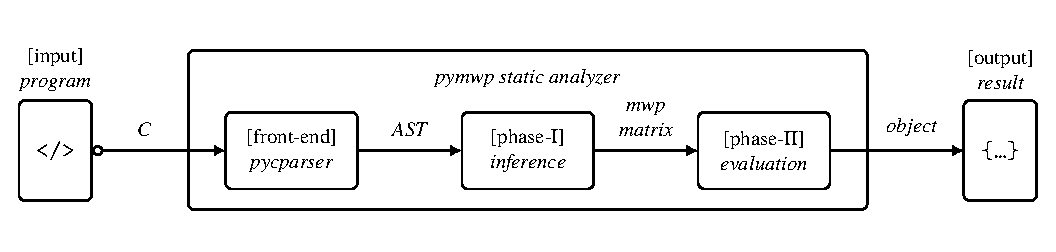
\includegraphics[width=\textwidth,keepaspectratio]{fig_pymwp}
\caption[The pymwp static analyzer workflow]{
The pymwp\index{pymwp} static analyzer workflow.
pymwp analyzes a C\index{C} program
and produces a result with information about the program's variable value growth.
If the program is derivable\index{derivability}, the result contains mwp-bounds\index{mwp-bound} for all variables.
Otherwise, the result identifies the variables with problematic data flows that cause derivation failure.
}\label{fig:pymwp}
\end{figure}

\paragraph*{Postconditions via mwp-bounds.}\index{mwp-bound}
The most recent development applies the flow calculus\index{mwp-calculus} to specification inference, namely postconditions~\cite{rusch2025}.
This ia new use-case, shifting the focus form static analysis toward formal verification.
Technically it introduces three flow calculus\index{mwp-calculus} enhancements:
projecting the mwp analysis on individual variables, improving the derivation failure handling strategy, an evaluation strategy to obtain optimal mwp-bounds\index{mwp-bound} through a query procedure.
For example, it permits inferring mwp-bounds\index{mwp-bound} of some variables in presence of whole-program derivation failure.
Due to focus on verifying numerical loops, the programming language is restricted to a language of loops.
The language adjustment is now a prerequisite to obtain the technical enhancements.
The loop analysis variant is implemented in pymwp\index{pymwp} as a special mode called mwp\(_\ell\).

\afterpage{%
\clearpage
\begin{landscape}
\begin{table}[p!]
\begin{NiceTabularX}{\hsize}{XXllll}
\toprule
  & & \textbf{The original} & \textbf{The enhanced} & \textbf{The pymwp} & \textbf{Postconditions} \\
\textbf{Phase} & \textbf{Description} & \textbf{flow calculus} & \textbf{\textsc{mwp}\(^\infty\) calculus} & \textbf{static analyzer} & \textbf{via mwp-bounds} \\
\midrule
  & Motivation & complexity theory & toward static analysis & static analysis & verification \\
\textsc{analysis input}
  & Language & \(\mathcal{L}\) (baseline)\smtabularnote{A language is similar to IMP of~\textcite{nielson2010,cpierce20221}.} & \(\mathcal{L} + f +\) recursion & \(\mathcal{L} \mapsto \) C99 & loops \(\subset \mathcal{L}\) \\
\textsc{analysis procedure}
  & Calculus variant & \textsc{mwp} & \textsc{mwp}\(^\infty\) & \textsc{mwp}\(^\infty\) & \textsc{mwp}\(^\infty\) \\
  & Matrix type & simple flows & complex & complex & complex \\
  & Matrix count & 0--\(3^k\) & 1 & 1 & 1 \\
  & Failure recovery & complete restart & \(\infty\) & \(\infty\) & \(\infty\) \\
  & Feedback on failure & none & none & failing variables & failing variables \\
\textsc{analysis output}
  & Bounds discovery & immediate & brute force & evaluation & evaluation \\
  & Generated bound & arbitrary & exists (y/n)\smtabularnote{Analysis determines if a bound exists, but does not provide bounds by default.} & arbitrary & optimal \\
  & Bounds granularity & whole-program & whole-program & whole-program & variables \\
  & Implementation & none & pymwp 0.1.6 & pymwp 0.4.2 & mwp\(_\ell\) 0.5.4 \\
\bottomrule
\end{NiceTabularX}
\caption[Technical developments of the flow calculus of mwp-bounds]
{Comparison of technical developments and features in works extending the flow calculus of mwp-bounds.}
\label{tab:evo}
\index{imperative programs}
\index{complexity theory}
\index{mwp-calculus}
\index{pymwp}
\index{C}
\end{table}
\end{landscape}}

\paragraph*{Open problems for future developments.}
Throughout the technical progression, the class of programs covered by the analysis has remained similar;
with small adjustments.
The semantic property of interest, variable value growth \wrt inputs, is never lost nor altered.
% -- the goal is consistently bounding variable value growth \wrt inputs.
Therefore, the flow calculus\index{mwp-calculus} input/output behavior has remained the same.
All notable changes concern the mechanics of the analysis and how to improve the process by which the analysis arrives to its conclusion.
In the original mwp-calculus\index{mwp-calculus}, determining program derivability\index{derivability} is an NP-complete\ccxi{np} problem.
It is unknown if the efficiency has changed following the technical advancements.

Among the remaining open problems are:
\begin{enumerate*}
\item extending the imperative language\index{imperative programs} to cover a larger class of programs,
\item formally verifying the flow calculus\index{mwp-calculus} for obtain a rigorous soundness guarantee (\cf~\autoref{certcpx}),
\item exploring the extended analysis applications, and
\item enhancing the precision of the flow calculus\index{mwp-calculus}.
\end{enumerate*}
Matrix construction is currently the most costly analysis phase.
It is possible to design data flows that make program analysis inefficient due to the resulting matrix size.
More effort is needed to scale the analysis to such inputs.

\subsubsection{Technical Details of Program Analysis}
\label{mwp-analysis}

The flow calculus\index{mwp-calculus} provides a static technique for analyzing programs written in an imperative language\index{imperative programs}.
Through its inference rules\index{inference rule}, the analysis assigns coefficients\index{flow coefficient} to program commands to determine if the program is derivable\index{derivability}.
This section gives an overview of the program analysis mechanics that suffices to understand the derivation examples that follow.
We present the original flow calculus\index{mwp-calculus}, because it generates mwp-matrices of simple coefficients which are easier to present and discuss on paper.
In contrast, the \textsc{mwp}\(^\infty\) calculus\index{mwp-calculus} generates complex mwp-matrices that requires two program analysis phases, for mwp-matrix\index{mwp-matrix} construction and evaluation.
For the best exposition of how to construct complex mwp-matrices see~\aref{sec:fscd}.
The evaluation procedure that extracts mwp-bounds\index{mwp-bound} from complex mwp-matrices is best described in~\autoref{sec:postcond}.

\paragraph*{An imperative programming language.}
The inputs of the analysis are specified in a simple imperative language (referred to as \pr|Imp| in code listings).
Because the language and semantics are defined in~\autoref{sec:postcond} and~\aref{sec:fscd}, they are not repeated here.
A \emph{program} is a sequence of commands.
A program manipulates sequentially a fixed number of natural number variables, with conditional branching and iteration permitted.
Control expressions in \pr|if| statements and \pr|while| loops do not matter;
all branches are analyzed and \pr|while| loops are over-approximated to iterate infinitely.
Conventionally, a program in the flow calculus\index{mwp-calculus} corresponds to a procedure.
Although simple, the imperative language\index{imperative programs} captures a core fragment of mainstream programming languages,
like C\index{C}
and  Java\index{Java};
and makes all languages that share the same core analyzable.

\paragraph*{The mwp-matrix algebra.}\index{mwp-matrix}
We use the definitions from the original flow calculus\index{mwp-calculus}~\cite{jones2009}.
The mwp-matrix algebra provides a mathematical framework for tracking variable value growth.

\begin{description}
\item[Elements.]
The mwp-matrix\index{mwp-matrix} elements are coefficients\index{flow coefficient} (or \emph{scalars}) in \(\mathcal{V} = \{ 0, m, w, p \} \).
The elements in \(\mathcal{V}\) are ordered \( 0 < m < w < p \) and letters \(\alpha, \beta, \gamma, \ldots\) denote elements in \(\mathcal{V}\).
The least upper bound of \(\alpha, \beta \in \mathcal{V}\) is denoted by \(\alpha + \beta\).
The operation evaluates to \(\alpha + \beta = \alpha\) if \(\alpha \geq \beta\), otherwise \(\alpha + \beta = \beta\).
The product of \(\alpha, \beta \in \mathcal{V}\) is denoted by \(\alpha \times \beta\) and
defined by  \(\alpha \times \beta = \alpha + \beta\) if \(\alpha, \beta \in \{m, w, p\}\),
otherwise \(\alpha \times \beta = 0\).

\begin{figure}
\begin{center}
$\begin{pNiceMatrix}[first-row,first-col]
& \prm{X}_0 & \hdots & \prm{X}_n \\
\prm{X}_0  & \ddots &      &  \iddots \\
\vdots  &  &  \alpha  & \\
\prm{X}_n & \iddots &      & \ddots
\end{pNiceMatrix}$
\end{center}
\caption[Variable-labels of an mwp-matrix]{Variable-labels of an mwp-matrix\index{mwp-matrix}.}
\label{fig:labels}
\end{figure}

\item[Matrices.]
For a program with \(n\) variables, an mwp-matrix\index{mwp-matrix}
\item (denoted \(M, A, B, C, \ldots\)) is a \(n \times n\) matrix over \(\mathcal{V}\).
We use \(M_{ij}\) to denote the matrix element at \emph{row} \({i}\) and \emph{column} \({j}\).
A \emph{zero matrix}\index{zero matrix} is denoted by \({0}\) and defined by \(M=0\) iff \(M_{ij} = 0\) for all indices \(i, j\).
An \emph{identity matrix}\index{identity matrix} is denoted by \({1}\) and defined by \(M = 1\) iff \(M_{ij} = m\) for \(i = j\) and \(M_{ij} = 0\) for \(i \neq j\).
The matrices are labelled by the program variables, as shown in~\autoref{fig:labels}, though the labels are typically omitted for compactness in derivations.
If no labels are provided, we assume ascending alphabetical ordering of variables.

\item[Matrix operations.]\index{mwp-matrix}
The least upper bound \( A \oplus B \) of the matrices \(A\) and \(B\) is defined component wise,
\ie \(C = A \oplus B\) iff \(C_{ij} =A_{ij} + B_{ij}\) for \(i, j \in \{ 1,\ldots,n \}\).
The matrix product \( A \otimes B \) of the matrices \(A\) and \(B\) is defined by \(M = A \otimes B \) iff \(M_{ij} = \Sigma_{k=1\ldots n} A_{ik} \times B_{kj}\), \ie standard matrix multiplication.
The closure (fixed point) of the matrix \(M\) is denoted by \(M^*\) and
defined as an infinite sum \[M^* = 1 \oplus M \otimes M^2 \oplus M^3 \oplus \ldots \]
\end{description}

\paragraph*{The inference rules of the mwp-calculus.}
\index{inference rule}
\index{mwp-calculus}

The inference rules\index{inference rule} of the mwp-calculus\index{mwp-calculus} \cf~\autoref{fig:jkrules} specify how different program operations impact variable value growth during computation.
Effectively, they provide the mechanics for connecting the mwp-matrix\index{mwp-matrix} algebra with imperative programs\index{imperative programs}.

\begin{figure}[p!]
    \begin{subfigure}{\textwidth}
        \begin{center}
            \begin{tabular}{l}
                \begin{prooftree}[small]
                    \infer0[E1]{ \vdashJK \text{\pr|Xi|} : \{_{\text{\,\pr|i|}}^{m}\}}
                \end{prooftree}
                \hspace{2em}
                \begin{prooftree}[small]
                    \infer0[E2]{ \vdashJK \text{\pr|e|} : \{_{\text{\,\pr|i|}}^{w} \mid \text{\pr|Xi|} \in \var(\text{\pr|e|}) \}}
                \end{prooftree}
            \end{tabular}
        \end{center}
    \end{subfigure}
    \\[1.2em]
    \begin{subfigure}{\textwidth}
        \begin{center}
            \begin{tabular}{l}
                \begin{prooftree}[small]
                    \hypo{\vdashJK \text{\pr{Xi}} : V_1}
                    \hypo{\vdashJK \text{\pr{Xj}} : V_2}
                    \infer[left label={\(\star\in\{+, -\}\)}]2[E3]{\vdashJK \text{\pr|Xi $\star$ Xj|} : pV_1 \oplus V_2}
                \end{prooftree}
                \hspace{1em}
                \begin{prooftree}[small]
                    \hypo{\vdashJK \text{\pr{Xi}} : V_1}
                    \hypo{\vdashJK \text{\pr{Xj}} : V_2}
                    \infer[left label={\(\star\in\{+, -\}\)}]2[E4]{\vdashJK \text{\pr|Xi $\star$ Xj|} : V_1 \oplus pV_2}
                \end{prooftree}
            \end{tabular}
        \end{center}
        \caption{Rules for assigning vectors to expressions}
        \label{fig:rules-expressions}
    \end{subfigure}
    \\[3em]
    \begin{subfigure}{\textwidth}
        \begin{centering}
            \begin{prooftree}[small]
                \infer0[S]{ \vdashJK \text{\pr|skip|} : \mathbf{1} }
            \end{prooftree}
            \hspace{3em}
            \begin{prooftree}[small]
                \hypo{ \vdashJK \text{\pr{e}} : V}
                \infer1[A]{\vdashJK \text{\pr|Xj = e|} : \mathbf{1} \xleftarrow{\text{\pr|j|}} V}
            \end{prooftree}
            \hspace{3em}
            \begin{prooftree}[small]
                \hypo{ \vdashJK \text{\pr{C1}} : M_1}
                \hypo{ \vdashJK \text{\pr{C2}} : M_2}
                \infer2[C]{\vdashJK \text{\pr{C1;C2}} : M_1 \otimes M_2}
            \end{prooftree}
            \\[1.2em]
            \begin{prooftree}[small]
                \hypo{ \vdashJK \text{\pr{C1}} : M_1}
                \hypo{ \vdashJK \text{\pr{C2}} : M_2}
                \infer2[I]{\vdashJK \text{\pr|if b then C1 $\text{\hspace{.3em}}$ else C2|} : M_1 \oplus M_2}
            \end{prooftree}
            \\[1.2em]
            \begin{prooftree}[small]
                \hypo{\vdashJK \text{\pr|C|} : M}
                \infer[left label={\(\forall i, M_{ii}^* = m\)}]1[L]{\vdashJK \text{\pr|loop Xl \{C\}|} : M^* \oplus \{_{\text{\pr|l|}}^{p}\rightarrow j \mid \exists i, M_{ij}^* = p\}}
            \end{prooftree}
            \\[1.2em]
            \begin{prooftree}[small]
                \hypo{\vdashJK \text{\pr|C|} : M}
                \infer[left label={\(\forall i, M_{ii}^* = m\) and \(\forall i, j, M^*_{ij} \neq p\)}]1[W]{\vdashJK \text{\pr|while b do  \{C\}|} : M^*}
            \end{prooftree}
            \caption{Rules for assigning matrices to commands}
            \label{fig:rules-commands}
        \end{centering}
    \end{subfigure}
    \caption[The inference rules of the original mwp-calculus]
    {The nondeterministic inference rules of the original mwp-calculus.}
    \label{fig:jkrules}\index{inference rule}\index{nondeterminism}
\end{figure}

\begin{description}
\item[Expressions.]
An \emph{expression} \pr|e| is assigned a vector \(V\) of coefficients\index{flow coefficient} \(\prm{e} : V\).
The rules for analysing expressions, E1--E4, are defined in~\autoref{fig:rules-expressions}.
The notation \(\{_{i}^{\alpha}\}\) means a vector with \(\alpha\) in its \(i^\text{th}\) row and $0$ everywhere else, and \(\var(\prm{e})\) means variables occurring in \pr|e|.
The product \(\alpha V\), where \(\alpha\) is a coefficient\index{flow coefficient} and \(V\) is a vector, is defined by
standard scalar multiplication of the vector elements.
Observe that there are 3 ways to analyze a binary operation.
This is the source of nondeterminism\index{nondeterminism} in the flow calculus\index{mwp-calculus}.
For \(k\) binary operation in the input program, there are \(3^k\) different derivation paths to analyze.
\item[Commands.]
A \emph{command} \pr|C| is assigned a (\(n \times n\)) matrix\index{mwp-matrix} \(M\) of coefficients\index{flow coefficient} \(\prm{C} : M\).
The rules for analysing commands are defined in~\autoref{fig:rules-commands}.
The notation \(M \xleftarrow{j} V\) means replacing in matrix $M$ the \(j^\text{th}\) column vector by $V$.
The notation \(_{\text{\pr|l|}}^{p}\rightarrow j\) means adding coefficient \(p\) in column \(j\) at row \pr|l|,
where \pr|l| is the column index of the loop guard variable\index{guard variable} \pr|Xl|.
\end{description}
The assignment rule A has the effect that the \emph{source} variables in the assignment expression impact the value growth of the assignment \emph{target}.
By the composition rule C, the impact of a command sequence is the product of the mwp-matrices\index{mwp-matrix} of the commands.
Since matrix multiplication is not commutative, the command order is relevant in mwp-calculus\index{mwp-calculus}.
The rule for \pr|if| statements accounts for computations in both branches, irrespective or order.
Only the iterative commands, \pr|loop| and \pr|while| have side conditions.
This means if a derivation fails, the source of failure is an iteration command.
Similarly, proving that variable value growth is polynomially bounded is trivial in absence of iteration.
Between the two iteration commands, \pr|while| is less permissive as it does not permit any \(p\)-flows in the mwp-matrix\index{mwp-matrix}.
The \pr|skip| command is simply an identity matrix\index{identity matrix} and has no effect.
However, it is necessary to formally handle \eg an omitted \pr|else| branch.
The \pr|skip| also permits handling commands that have no impact on variable value growth,
but that occur in realistic programming languages, \eg assertions.


\paragraph*{The analysis procedure.}
Recall, a program is a sequence of commands.
Program analysis using the flow calculus\index{mwp-calculus} requires inspecting the sequence of commands,
applying the inference rules\index{inference rule}, and composing the mwp-matrices of the commands.
Each command is either derivable\index{derivability} or raises a derivation failure.

In practice, the analysis is performed over the program's abstract syntax tree\index{abstract syntax tree} (AST).
Since a tree is a hierarchical structure, the analysis proceeds in depth-first order, like evaluation of a sequential program.
The derivation examples in~\autoref{mwp-derivations} demonstrate the concept.
For simplicity, in describing the analysis procedure we assume a flattened parse-tree of commands.


Let \(P = (\prm{C}_0,\prm{C}_1,\ldots,\prm{C}_m) \) be a program in an imperative language\index{imperative programs} where \(m \geq 1\).
A generalized program analysis proceeds by~\autoref{alg:prog}, with the analysis of individual commands is described in~\autoref{alg:comms}\footnote{
    Detailed implementations of these algorithms are available in the pymwp\index{pymwp} source code as
    \href{https://github.com/statycc/pymwp/blob/40c9ceb644c734f15f82e63edc515716c4f35841/pymwp/analysis.py\#L118}
    {\pr|Analysis.cmds|} and
    \href{https://github.com/statycc/pymwp/blob/40c9ceb644c734f15f82e63edc515716c4f35841/pymwp/analysis.py\#L185}{\pr|Analysis.compute\_relation|}.}.
Conceptually, the program analysis is straightforward: compose the mwp-matrices of commands in the order they appear in the AST\@.
However, in practice care is needed to account for the exponential number of derivation paths
and handling potential derivation failure.
Failure handling varies between the different versions of the flow analysis (\cf~\autoref{tab:evo});
therefore, the specifics are omitted here.
The \textsc{mwp}\(^\infty\) variant of the flow calculus\index{mwp-calculus} internalizes the failure and always returns an mwp-matrix\index{mwp-matrix}.

\begin{algorithm}
    \caption[Program analysis with flow calculus of mwp-bounds]
    {Program analysis with flow calculus of mwp-bounds.}\label{alg:prog}
    \textbf{Input}: sequence of commands \pr|P| \\
    \textbf{Output}: mwp-matrix\index{mwp-matrix} \(M\) or failure
    \begin{algorithmic}[1]
        \State Take the first command \(\prm{C}_0\) in \pr|P|
        \State Analyze \(\prm{C}_0\) by \autoref{alg:comms} to obtain \(M\)
        \State (Maybe signal failure)
        \For{Commands \(n = 1 \ldots m\)}
            \State Analyze \(\prm{C}_n\) by \autoref{alg:comms}
            \State (Maybe signal failure)
            \State Compose \(M = M \circ M_n \) by rule C
        \EndFor
        \State \Return mwp-matrix \(M\) \Comment{\(\vdash \prm{P} : M\)}
    \end{algorithmic}
\end{algorithm}

\begin{algorithm}
    \caption[Command analysis with flow calculus of mwp-bounds]
    {Command analysis with flow calculus of mwp-bounds.}\label{alg:comms}
    \textbf{Input}: command \pr|C| \\
    \textbf{Output}: mwp-matrix\index{mwp-matrix} \(M\) or failure
    \begin{algorithmic}[1]
        \State Analyze expressions in \pr|C| by rules E1-E4
        \State Analyze \pr|C| by rules A-W, possibly recursively
        \State (Maybe signal failure)
        \State \Return \(M\) \Comment{\(\vdash\prm{C} : M\)}
    \end{algorithmic}
\end{algorithm}

\subsubsection{Illustrative Derivations I: The Range of Analysis Outcomes}\label{mwp-derivations}

\begin{example}[Polynomially bounded program is derivable]\label{ex:bounds1T}
Recall the program from~\autoref{ex:bounds1},

%! suppress = FileNotFound
\captionsetup{type=lstlisting}
\impinputlisting[][numbers=none]{derivable.imp}
\captionof{lstlisting}[Derivable program]{A derivable program.}
\label{lst:ex-derivable}

The conclusion about derivability\index{derivability} can be reached by $3^2 = 9$ distinct derivations,
one of which is shown below.

\begin{center}\begin{prooftree}
\infer0[E1]{\vdashJK \text{\pr|X2|} : \mat{0\\m\\0}}
\infer0[E1]{\vdashJK \text{\pr|X3|} : \mat{0\\0\\m}}
\infer2[E4]{\vdashJK \text{\pr|X2+X3|} : \mat{0\\m\\p}}
\infer1[A]{ \vdashJK \text{\pr|X1=X2+X3|} : \mat{0&0&0 \\ m&m&0 \\p&0&m}}
\infer0[E1]{\vdashJK \text{\pr|X1|} : \mat{m\\0\\0}}
\infer0[E1]{\vdashJK \text{\pr|X1|} : \mat{m\\0\\0}}
\infer2[E4]{\vdashJK \text{\pr|X1+X1|} : \mat{p\\0\\0}}
\infer1[A]{ \vdashJK \text{\pr|X1=X1+X1|} : \mat{p&0&0 \\ 0&m&0 \\0&0&m}}
\infer2[C]{\vdashJK \text{\pr|X1=X2+X3; X1=X1+X1|} :  \mat{0&0&0 \\ p&m&0 \\p&0&m}}
\end{prooftree}\end{center}

The mwp-bounds\index{mwp-bound} are obtained column-wise from the concluding mwp-matrix\index{mwp-matrix}, cf.~\autoref{interpreting-bounds}.
For \pr|X1|, the vector \(\mat{0\\p\\p}\)
corresponds to \(x_1' \leq \max(0) + \prm{X2}\times\prm{X3}\) and simplifies to \(x_1' \leq\prm{X2}\times\prm{X3}\).
The mwp-bound\index{mwp-bound} is not as tight as possible (expression \pr|X2+X3| would be an improvement),
but discovering a better one requires exploring the derivation paths exhaustively.
Variables \pr|X2| and \pr|X3| obtain the same mwp-bounds\index{mwp-bound} in every derivation.
For \pr|X2|, the vector \(\mat{0\\m\\0}\) gives an mwp-bound\index{mwp-bound} \(x_2' \leq\prm{X2}\),
and for \pr|X3|, the vector \(\mat{0\\0\\m}\) gives \(x_3' \leq\prm{X3}\).
The program bound is a conjunction of the variables' mwp-bounds\index{mwp-bound}, \ie
\(x_1'\leq\prm{X2}\times\prm{X3} \land x_2' \leq\prm{X2} \land x_3' \leq\prm{X3}\).
\end{example}

\begin{example}[Failing program admits no derivation]\label{ex:bounds2F}
Consider the program fragment from~\autoref{ex:bounds2},

%! suppress = FileNotFound
\captionsetup{type=lstlisting}
\impinputlisting[][numbers=none]{failing.imp}
\captionof{lstlisting}[Loop that always fails the derivation]{A loop that always fails the derivation.}
\label{lst:ex-failing}

The command \pr|X1=X1+X1| admits three derivations.

\begin{center}
\begin{prooftree}
\infer0[E1]{ \vdashJK \text{\pr|X1|} : \mat{m\\0}}
\infer1[E3]{ \vdashJK \text{\pr|X1+X1|} : \mat{p\\0}}
\infer1[A]{ \vdashJK \text{\pr|X1=X1+X1|} : \mat{p&0\\0&m}}
\end{prooftree}
\hfill
\begin{prooftree}
\infer0[E1]{ \vdashJK \text{\pr|X1|} : \mat{m\\0}}
\infer1[E4]{ \vdashJK \text{\pr|X1+X1|} : \mat{p\\0}}
\infer1[A]{ \vdashJK \text{\pr|X1=X1+X1|} : \mat{p&0\\0&m}}
\end{prooftree}
\hfill
\begin{prooftree}
\infer0[E2]{ \vdashJK \text{\pr|X1+X1|} : \mat{w\\0}}
\infer1[A]{ \vdashJK \text{\pr|X1=X1+X1|} : \mat{w&0\\0&m}}
\end{prooftree}
\end{center}

The next step in the derivation requires accounting for the enclosing loop by applying the rule L\@.
The application involves computing the closure (fixed point) \(M^{*}\) of the mwp-matrix\index{mwp-matrix} assigned to
the body command \pr|X1=X1+X1|.
In this instance, the fixed point computation does not change the mwp-matrix\index{mwp-matrix} coefficients\index{flow coefficient}.
The L side condition is \(\forall i, M_{ii}^* = m\).
That is, it requires \(m\)-coefficients on the diagonal of \(M^{*}\).
None of the derivations satisfy the side condition, therefore the program is not derivable\index{derivability}.
Although the analysis focused only on a program fragment,
the complete program fails because it contains a command that is not derivable\index{derivability}.
\end{example}

\begin{example}[Derivability in presence of partial derivation failure]\label{ex:partial}
\index{derivability}
Consider the following program, that is a slightly modified version of~\autoref{ex:bounds2F},

%! suppress = FileNotFound
\captionsetup{type=lstlisting}
\impinputlisting[][numbers=none]{partial.imp}
\captionof{lstlisting}[Loop that fails for some derivation paths]{A loop that fails for some derivation paths.}
\label{lst:partial-fail}

The body of the \pr|loop| command admits three different derivations,
obtained by applying the tule A to one of the three derivation of the expression
\pr|X1+X2|, that we name \(\pi_0\), \(\pi_1\) and \(\pi_2\):

\begin{center}
\scalebox{0.85}{
\begin{prooftree}[small]
    \infer0[E1]{ \vdashJK \text{\pr|X1|} : \mat{m\\0\\0}}
    \infer0[E1]{ \vdashJK \text{\pr|X2|} : \mat{0\\m\\0}}
    \infer2[E3]{ \vdashJK \text{\pr|X1+X2|} : \mat{p\\m\\0}}
\end{prooftree}}
\hfill
\scalebox{0.85}{
\begin{prooftree}[small]
    \infer0[E1]{ \vdashJK \text{\pr|X1|} : \mat{m\\0\\0}}
    \infer0[E1]{ \vdashJK \text{\pr|X2|} : \mat{0\\m\\0}}
    \infer2[E4]{ \vdashJK \text{\pr|X1+X2|} : \mat{m\\p\\0}}
\end{prooftree}}
\hfill
\scalebox{0.85}{
\begin{prooftree}[small]
    \infer0[E2]{ \vdashJK \text{\pr|X1+X2|} : \mat{w\\w\\0}}
\end{prooftree}}
\end{center}

From \(\pi_0\), the derivation of  \pr|loop X3 {X2=X1+X2}| can be
completed using A and L, but since L requires having only \(m\) coefficients
on the diagonal, \(\pi_1\) cannot be used to complete the derivation,
because of the \(p\) coefficient in a box below:

\begin{center}
\begin{prooftree}
\hypo{}
\ellipsis{\(\pi_0\)}{ \vdashJK \text{\pr|X1+X2|} : \mat{p\\m\\0}}
\infer1[A]{ \vdashJK \text{\pr|X2=X1+X2|} : \mat{m&p&0 \\ 0&m&0 \\0&0&m}}
\infer1[L]{ \vdashJK \text{\pr|loop X3 \{X2=X1+X2\}|} :  \mat{m&p&0 \\ 0&m&0 \\0&p&m}}
\end{prooftree}
\hspace{2em}
\begin{prooftree}
\hypo{}
\ellipsis{\(\pi_1\)}{ \vdashJK \text{\pr|X1+X2|} : \mat{m\\p\\0}}
\infer1[A]{ \vdashJK \text{\pr|X2=X1+X2|}: \mat{m&m&0 \\ 0& \boxed{p} &0 \\0&0&m}}
\end{prooftree}
\end{center}

Similarly, using A after \(\pi_2\) gives a \(w\) coefficient on the
diagonal and makes it impossible to use L, hence only one derivation for this program exists.
A single successful derivation is sufficient to make the input program derivable\index{derivability}.
\end{example}

\subsubsection{Illustrative Derivations II: Programs From the Tool User Guide}

The pymwp\index{pymwp} tool user guide, in ~\autoref{sec:toolguide}, discusses five cases of program analysis of programs written in C\index{C}.
The tool user guide gives the analyzer input and output and describes the rationale for the obtained result.
This section complements the tool user guide by showing the derivations behind those results.
To retail fidelity with the C\index{C} language examples,
we show inputs in C\index{C},
but implicitly convert them to the core imperative language\index{imperative programs} of the flow calculus\index{mwp-calculus}.
The examples omit function declarations since those are irrelevant for the analysis.

\begin{example}[Binary assignment]\label{ex:binassign}
The input program in~\autoref{lst:ex-assign} contains a single command.

\begin{center}
\begin{minipage}{\textwidth}
\captionsetup{type=lstlisting}
\cinputlisting{assign_expression.c}
\captionof{lstlisting}[Program with a single assignment]{A program with a single assignment.}
\label{lst:ex-assign}
\end{minipage}
\end{center}

The program has three derivations and all of them succeed.
One derivation instance is shown below.

\begin{center}\begin{prooftree}
\infer0[E1]{\vdashJK \text{\pr|Y1|} : \mat{m\\0}}
\infer0[E1]{\vdashJK \text{\pr|Y1|} : \mat{m\\0}}
\infer2[E3]{\vdashJK \text{\pr|Y1+Y1|} : \mat{p\\0}}
\infer1[A]{ \vdashJK \text{\pr|Y2=Y1+Y1|} : \mat{0&p \\m&0}}
\end{prooftree}\end{center}
The program bound is a \(y_1'\leq\prm{Y1} \land y_2' \leq\prm{Y1}\).
\end{example}

\begin{example}[Exponential Program]\label{ex:expprog}
The input program is in~\autoref{lst:ex-exponent2}.

\begin{center}
\begin{minipage}{\textwidth}
\captionsetup{type=lstlisting}
\cinputlisting{exponent2.c}
\captionof{lstlisting}[Program with exponential variable value growth]{A program with exponential variable value growth.}
\label{lst:ex-exponent2}
\end{minipage}
\end{center}

\paragraph*{Step 1.} Analyze the command \pr|result = result * base| (simplified to \pr|r=r*b| in the following).
It admits three derivations (\(\pi_0\), \(\pi_1\) and \(\pi_2\)).

\begin{center}
\scalebox{0.85}{
\begin{prooftree}[small]
\infer0[E1]{ \vdashJK\text{\pr|r|} : \mat{0\\0\\0\\m}}
\infer0[E1]{ \vdashJK\text{\pr|b|} : \mat{m\\0\\0\\0}}
\infer2[E3]{ \vdashJK\text{\pr|r*b|} : \mat{p\\0\\0\\m}}
\infer1[A]{ \vdashJK\text{\pr|r=r*b|} : \mat{m&0&0&p\\0&m&0&0\\0&0&m&0\\0&0&0&m}}
\end{prooftree}}
\hfill
\scalebox{0.85}{
\begin{prooftree}[small]
\infer0[E1]{ \vdashJK \text{\pr|r|} : \mat{0\\0\\0\\m}}
\infer0[E1]{ \vdashJK \text{\pr|b|} : \mat{m\\0\\0\\0}}
\infer2[E4]{ \vdashJK \text{\pr|r*b|} : \mat{m\\0\\0\\p}}
\infer1[A]{ \vdashJK\text{\pr|r=r*b|} : \mat{m&0&0&m\\0&m&0&0\\0&0&m&0\\0&0&0&p}}
\end{prooftree}}
\hfill
\scalebox{0.85}{
\begin{prooftree}[small]
\infer0[E2]{ \vdashJK \text{\pr|r*b|} : \mat{w\\0\\0\\w}}
\infer1[A]{ \vdashJK\text{\pr|r=r*b|} : \mat{m&0&0&w\\0&m&0&0\\0&0&m&0\\0&0&0&w}}
\end{prooftree}}
\end{center}

\paragraph*{Step 2.} Analyze command \pr|i=i+1|.
Similarly, it admits three derivations (\(\pi_3\), \(\pi_4\) and \(\pi_5\)).

\begin{center}
\scalebox{0.85}{
\begin{prooftree}[small]
\infer0[E1]{ \vdashJK \text{\pr|i|} : \mat{0\\0\\m\\0}}
\infer0[E1]{ \vdashJK \text{\pr|1|} : \mat{0\\0\\0\\0}}
\infer2[E3]{ \vdashJK \text{\pr|i+1|} : \mat{0\\0\\p\\0}}
\infer1[A]{ \vdashJK \text{\pr|i=i+1|} : \mat{m&0&0&0\\0&m&0&0\\0&0&p&0\\0&0&0&m}}
\end{prooftree}}
\hfill
\scalebox{0.85}{
\begin{prooftree}[small]
\infer0[E1]{ \vdashJK \text{\pr|i|} : \mat{0\\0\\m\\0}}
\infer0[E1]{ \vdashJK \text{\pr|1|} : \mat{0\\0\\0\\0}}
\infer2[E4]{ \vdashJK \text{\pr|i+1|} : \mat{0\\0\\m\\0}}
\infer1[A]{ \vdashJK \text{\pr|i=i+1|} : \mat{m&0&0&0\\0&m&0&0\\0&0&m&0\\0&0&0&m}}
\end{prooftree}}
\hfill
\scalebox{0.85}{
\begin{prooftree}[small]
\infer0[E2]{ \vdashJK \text{\pr|i+1|} : \mat{0\\0\\w\\0}}
\infer1[A]{ \vdashJK \text{\pr|i=i+1|} : \mat{m&0&0&0\\0&m&0&0\\0&0&w&0\\0&0&0&m}}
\end{prooftree}}
\end{center}

\paragraph*{Step 3.} Compose the body commands, \pr|r=r*b; i=i+1|.
There are 9 different combinations, by the derivation choices made in the previous steps.

\begin{center}
\begin{prooftree}
\hypo{}\ellipsis{\(\pi_0\times\pi_3\)}{ }
\infer1[C]{ \vdashJK \text{\pr|B|} : \mat{m&0&0&p\\0&m&0&0\\0&0&p&0\\0&0&0&m}}
\end{prooftree}
\hfill
\begin{prooftree}
\hypo{}\ellipsis{\(\pi_0\times\pi_4\)}{ }
\infer1[C]{ \vdashJK \text{\pr|B|} : \mat{m&0&0&p\\0&m&0&0\\0&0&m&0\\0&0&0&m}}
\end{prooftree}
\hfill
\begin{prooftree}
\hypo{}\ellipsis{\(\pi_0\times\pi_5\)}{ }
\infer1[C]{ \vdashJK \text{\pr|B|} : \mat{m&0&0&p\\0&m&0&0\\0&0&w&0\\0&0&0&m}}
\end{prooftree}
\\[1em]
\begin{prooftree}
\hypo{}\ellipsis{\(\pi_1\times\pi_3\)}{ }
\infer1[C]{ \vdashJK \text{\pr|B|} : \mat{m&0&0&m\\0&m&0&0\\0&0&p&0\\0&0&0&p}}
\end{prooftree}
\hfill
\begin{prooftree}
\hypo{}\ellipsis{\(\pi_1\times\pi_4\)}{ }
\infer1[C]{ \vdashJK \text{\pr|B|} : \mat{m&0&0&m\\0&m&0&0\\0&0&m&0\\0&0&0&p}}
\end{prooftree}
\hfill
\begin{prooftree}
\hypo{}\ellipsis{\(\pi_1\times\pi_5\)}{ }
\infer1[C]{ \vdashJK \text{\pr|B|} : \mat{m&0&0&m\\0&m&0&0\\0&0&w&0\\0&0&0&p}}
\end{prooftree}
\\[1em]
\begin{prooftree}
\hypo{}\ellipsis{\(\pi_2\times\pi_3\)}{ }
\infer1[C]{ \vdashJK \text{\pr|B|} : \mat{m&0&0&w\\0&m&0&0\\0&0&p&0\\0&0&0&w}}
\end{prooftree}
\hfill
\begin{prooftree}
\hypo{}\ellipsis{\(\pi_2\times\pi_4\)}{ }
\infer1[C]{ \vdashJK \text{\pr|B|} : \mat{m&0&0&w\\0&m&0&0\\0&0&m&0\\0&0&0&w}}
\end{prooftree}
\hfill
\begin{prooftree}
\hypo{}\ellipsis{\(\pi_2\times\pi_5\)}{ }
\infer1[C]{ \vdashJK \text{\pr|B|} : \mat{m&0&0&w\\0&m&0&0\\0&0&w&0\\0&0&0&w}}
\end{prooftree}
\end{center}

\paragraph*{Step 4.}
Apply rule W to account for the enclosing \pr|while| loop.
It requires first computing mwp-matrix\index{mwp-matrix}  closure \(M^{*}\) for the body command.
The side conditions is \(\forall i, M_{ii}^* = m\) and \(\forall i, j, M^*_{ij} \neq p\).
That is, the rule can be applied when only $m$-coefficients appear on the diagonal
and no $p$-coefficients occur anywhere in the mwp-matrix\index{mwp-matrix} .
In every derivation, the mwp-matrix\index{mwp-matrix}  violates the side condition by the boxed coefficients\index{flow coefficient}.

\begin{center}
\begin{prooftree}
\hypo{}\ellipsis{\(\pi_0\times\pi_3\)}{M^{*} = \mat{m&0&0&\boxed{p}\\0&m&0&0\\0&0&\boxed{p}&0\\0&0&0&m}}
\end{prooftree}
\hfill
\begin{prooftree}
\hypo{}\ellipsis{\(\pi_0\times\pi_4\)}{M^{*} = \mat{m&0&0&\boxed{p}\\0&m&0&0\\0&0&m&0\\0&0&0&m}}
\end{prooftree}
\hfill
\begin{prooftree}
\hypo{}\ellipsis{\(\pi_0\times\pi_5\)}{M^{*} = \mat{m&0&0&\boxed{p}\\0&m&0&0\\0&0&\boxed{w}&0\\0&0&0&m}}
\end{prooftree}
\\[1em]
\begin{prooftree}
\hypo{}\ellipsis{\(\pi_1\times\pi_3\)}{M^{*} = \mat{m&0&0&m\\0&m&0&0\\0&0&\boxed{p}&0\\0&0&0&\boxed{p}}}
\end{prooftree}
\hfill
\begin{prooftree}
\hypo{}\ellipsis{\(\pi_1\times\pi_4\)}{M^{*} = \mat{m&0&0&m\\0&m&0&0\\0&0&m&0\\0&0&0&\boxed{p}}}
\end{prooftree}
\hfill
\begin{prooftree}
\hypo{}\ellipsis{\(\pi_1\times\pi_5\)}{M^{*} = \mat{m&0&0&m\\0&m&0&0\\0&0&\boxed{w}&0\\0&0&0&\boxed{p}}}
\end{prooftree}
\\[1em]
\begin{prooftree}
\hypo{}\ellipsis{\(\pi_2\times\pi_3\)}{M^{*} = \mat{m&0&0&w\\0&m&0&0\\0&0&\boxed{p}&0\\0&0&0&\boxed{w}}}
\end{prooftree}
\hfill
\begin{prooftree}
\hypo{}\ellipsis{\(\pi_2\times\pi_4\)}{M^{*} = \mat{m&0&0&w\\0&m&0&0\\0&0&m&0\\0&0&0&\boxed{w}}}
\end{prooftree}
\hfill
\begin{prooftree}
\hypo{}\ellipsis{\(\pi_2\times\pi_5\)}{M^{*} = \mat{m&0&0&w\\0&m&0&0\\0&0&\boxed{w}&0\\0&0&0&\boxed{w}}}
\end{prooftree}
\end{center}

\paragraph*{Step 5.} We conclude the input program is not derivable\index{derivability}.
\end{example}

\begin{example}[While analysis]\label{ex:while1}
The input program, that we will refer to as \(P\), is

\begin{center}
\begin{minipage}{\textwidth}
\captionsetup{type=lstlisting}
\cinputlisting{notinfinite3.c}
\captionof{lstlisting}[Program with a \texttt{while} loop]{A program with a \texttt{while} loop.}
\label{lst:ex-notinfinite3}
\end{minipage}
\end{center}

The tool user guide reveals that the program is derivable\index{derivability}.
Compared to derivation failure that requires exploring all derivation choices,
a derivable\index{derivability} program simply requires showing one successful derivation.
For presentation reasons, we show the two branches of the derivation tree individually.

\paragraph*{Step 1.} The derivation of the \pr|if| command (\(\pi_0\)){ }is straightforward.
Observe that the control expression of the \pr|if| statement has no impact on the constructed mwp-matrix\index{mwp-matrix}.

\begin{center}
\begin{prooftree}
\infer0[E1]{\vdashJK \text{\pr|X1|} : \mat{0\\m\\0\\0}}
\infer0[E1]{\vdashJK \text{\pr|X2|} : \mat{0\\0\\m\\0}}
\infer2[E4]{\vdashJK \text{\pr|X2+X1|} : \mat{0\\m\\p\\0}}
\infer1[A]{ \vdashJK \text{\pr|X1=X2+X1|} : \mat{m&0&0&0\\0&m&0&0\\0&p&m&0\\0&0&0&m}}
\infer0[E1]{\vdashJK \text{\pr|X3|} : \mat{0\\0\\0\\m}}
\infer0[E1]{\vdashJK \text{\pr|X2|} : \mat{0\\0\\m\\0}}
\infer2[E4]{\vdashJK \text{\pr|X3+X2|} : \mat{0\\0\\m\\p}}
\infer1[A]{ \vdashJK \text{\pr|X2=X3+X2|} : \mat{m&0&0&0\\0&m&0&0\\0&0&m&0\\0&0&p&m}}
\infer2[I]{ \vdashJK \text{\pr|if(X1==1) \{ X1=X2+X1; X2=X3+X2 \}|} : \mat{m&0&0&0\\0&m&0&0\\0&p&m&0\\0&0&p&m}}
\end{prooftree}
\end{center}

\paragraph*{Step 2.} The derivation of the \pr|while| loop (\(\pi_1\)){ }is now permitted,
because the rule W side condition is not violated by any coefficient\index{flow coefficient}.

\begin{center}
\begin{prooftree}
\infer0[E1]{\vdashJK \text{\pr|X1|} : \mat{0\\w\\0\\0}}
\infer0[E1]{\vdashJK \text{\pr|X2|} : \mat{0\\0\\w\\0}}
\infer2[E4]{\vdashJK \text{\pr|X1+X2|} : \mat{0\\w\\w\\0}}
\infer1[A]{ \vdashJK \text{\pr|X0=X1+X2|} : \mat{0&0&0&0\\w&m&0&0\\w&0&m&0\\0&0&0&m}}
\infer1[W]{ \vdashJK \text{\pr|while(X0<10) X0=X1+X2 |} : \mat{m&0&0&0\\w&m&0&0\\w&0&m&0\\0&0&0&m}}
\end{prooftree}
\end{center}

\paragraph*{Step 3.} Composing the mwp-matrices of the two commands
gives an mwp-matrix\index{mwp-matrix} for the complete input program \(P\).
We conclude the syntactic data-flow relation\index{data flow relation} \(\vdash P : M \) holds.

\begin{center}
\begin{prooftree}
\hypo{}
\ellipsis{\(\pi_0\times\pi_1\)}{ }
\infer1[C]{\vdashJK P : \mat{m&0&0&0\\w&m&0&0\\p&p&m&0\\p&0&p&m}}
\end{prooftree}
\end{center}
If the program terminates\index{termination} for the input values of the variables (it does not terminate for all inputs),
the variable value growth is polynomially bounded.
The mwp-bounds\index{mwp-bound} of the variables are
\(x_0' \leq \max(\prm{X0},\prm{X1})+\prm{X2}\times\prm{X3}\) and
\(x_1' \leq \max(\prm{X1})+\prm{X2} \) and
\(x_2' \leq \max(\prm{X2})+\prm{X3} \) and
\(x_3' \leq \max(\prm{X3})\).
This program bound matches the result of the tool user guide.
\end{example}

\begin{example}[Infinite program]\label{ex:infprog}
The input program is

\begin{center}
\begin{minipage}{\textwidth}
\captionsetup{type=lstlisting}
\cinputlisting{infinite3.c}
\captionof{lstlisting}[\enquote{Infinite} program]{An \enquote{infinite} program.}
\label{lst:ex-infinite3}
\end{minipage}
\end{center}

This program is similar to~\autoref{ex:while1}, with only a small change to the \pr|while| loop.
From the previous example, the \pr|if| statement is derivable\index{derivability} as before by \(\pi_0\).
Letting \(\prm{C}_2\) represent the \pr|while| command, the mwp-matrix\index{mwp-matrix} closures \(M^{*}\) of \(\prm{C}_2\) are shown below.

\begin{center}
\begin{prooftree}
\hypo{}\ellipsis{E3}{M^{*} = \mat{m&0&0&0\\0&\boxed{p}&0&0\\0&m&m&0\\0&0&0&m}}
\end{prooftree}
\hfill
\begin{prooftree}
\hypo{}\ellipsis{E4}{M^{*} = \mat{m&0&0&0\\0&m&0&0\\0&\boxed{p}&m&0\\0&0&0&m}}
\end{prooftree}
\hfill
\begin{prooftree}
\hypo{}\ellipsis{E2}{M^{*} = \mat{m&0&0&0\\0&\boxed{w}&0&0\\0&w&m&0\\0&0&0&m}}
\end{prooftree}
\end{center}
Every \(M^{*}\) violates the side condition of rule W.
The problematic coefficient\index{flow coefficient} is boxed for emphasis.
The program is not derivable\index{derivability}.
\end{example}

\begin{example}[Challenge example]\label{ex:challange}
The input program has four top-level commands, identified by the circled annotations.

\begin{center}
\begin{minipage}{\textwidth}
\captionsetup{type=lstlisting}
\cinputlisting{dense_loop.c}
\captionof{lstlisting}[Challenge program whose derivability is unknown]{A challenge program whose derivability is unknown.}
\label{lst:maybe-derivable}
\end{minipage}
\end{center}

We will refer to these commands as \(\prm{C}_0\)--\(\prm{C}_3\) and their derivations as \(\pi_0\)--\(\pi_3\), respectively.
The program analysis proceeds in corresponding steps.
To ease presentation, we will analyze command composition after each individual command.

\paragraph*{Step 1.} Analyze command \(\prm{C}_0\) \ie the \pr|if-else| statement.

\begin{center}\begin{prooftree}
\infer0[E1]{\vdashJK \text{\pr|X0|} : \mat{m\\0\\0}}
\infer0[E1]{\vdashJK \text{\pr|X1|} : \mat{0\\m\\0}}
\infer2[E4]{\vdashJK \text{\pr|X0+X1|} : \mat{m\\p\\0}}
\infer1[A]{ \vdashJK \text{\pr|X2=X0+X1|} : \mat{m&0&m\\0&m&p\\0&0&0}}
\infer0[E1]{\vdashJK \text{\pr|X2|} : \mat{0\\0\\m}}
\infer0[E1]{\vdashJK \text{\pr|X1|} : \mat{0\\m\\0}}
\infer2[E4]{\vdashJK \text{\pr|X2+X1|} : \mat{0\\p\\m}}
\infer1[A]{ \vdashJK \text{\pr|X2=X2+X1|} : \mat{m&0&0\\0&m&p\\0&0&m}}
\infer2[I]{ \vdashJK \text{\pr|if(X0) X2=X0+X1; else X2=X2+X1|} : \mat{m&0&m\\0&m&p\\0&0&m}}
\end{prooftree}\end{center}

\paragraph*{Steps 2--3.} Analyze commands \(\prm{C}_1\) and \(\prm{C}_2\), \ie \pr|X0=X2+X1| and \pr|X1=X0+X2|.

\begin{center}
\begin{prooftree}
\infer0[E1]{\vdashJK \text{\pr|X2|} : \mat{0\\0\\m}}
\infer0[E1]{\vdashJK \text{\pr|X1|} : \mat{0\\m\\0}}
\infer2[E4]{\vdashJK \text{\pr|X2+X1|} : \mat{0\\p\\m}}
\infer1[A]{\vdashJK \text{\pr|X0=X2+X1|} : \mat{0&0&0\\p&m&0\\m&0&m}}
\end{prooftree}
\hfill
\begin{prooftree}
\infer0[E2]{\vdashJK \text{\pr|X0+X2|} : \mat{w\\0\\w}}
\infer1[A]{\vdashJK \text{\pr|X1=X0+X2|} : \mat{m&w&0\\0&0&0\\0&w&m}}
\end{prooftree}
\end{center}

\paragraph*{Steps 4.} Analyze command \(\prm{C}_3\) \ie the \pr|while| loop.

\begin{center}
\begin{prooftree}
\infer0[E2]{\vdashJK \text{\pr|X1+X0|} : \mat{w\\w\\0}}
\infer1[A]{\vdashJK \text{\pr|X2=X1+X0|} : \mat{m&0&w\\0&m&w\\0&0&0}}
\infer1[W]{ \vdashJK \text{\pr|while(X2) X2=X1+X0|} : \mat{m&0&w\\0&m&w\\0&0&m}}
\end{prooftree}
\end{center}

\paragraph*{Steps 5.} Compose the mwp-matrices of derivations \(\pi_0 \ldots \pi_3\).

\noindent\resizebox{\textwidth}{!}{\begin{prooftree}
\hypo{}\ellipsis{\(\pi_0\)}{\vdashJK \prm{C}_0 : \mat{m&0&m\\0&m&p\\0&0&m}}
\hypo{}\ellipsis{\(\pi_1\)}{\vdashJK \prm{C}_1 : \mat{0&0&0\\p&m&0\\m&0&m}}
\infer2[C]{ \vdashJK \prm{C}_0\prm{;}\prm{C}_1 : \mat{m&0&m\\p&m&p\\m&0&m}}
\hypo{}\ellipsis{\(\pi_2\)}{\vdashJK \prm{C}_2 : \mat{m&w&0\\0&0&0\\0&w&m}}
\infer2[C]{ \vdashJK \prm{C}_0\prm{;}\prm{C}_1\prm{;}\prm{C}_2 : \mat{m&w&m\\p&p&p\\m&w&m}}
\hypo{}\ellipsis{\(\pi_3\)}{\vdashJK \prm{C}_3  : \mat{m&0&w\\0&m&w\\0&0&m}}
\infer2[C]{ \vdashJK \prm{C}_0\prm{;}\prm{C}_1\prm{;}\prm{C}_2\prm{;}\prm{C}_3 :
\mat{m&w&w\\p&p&p\\m&w&w}}
\end{prooftree}}

\vspace{1em}\noindent
The derivation gives variable mwp-bounds\index{mwp-bound}
\(x_0' \leq \max(\prm{X0},\prm{X2})+\prm{X1}\) and
\(x_1' \leq \prm{X0}+\prm{X2}+\prm{X1}\) and
\(x_2' \leq \prm{X0}+\prm{X2}+\prm{X1}\).
The program has 81 admissible derivations in total.
\end{example}

\subsection{Literature Topic 4: Loop Transformations for Parallel Programming}\label{transforms}
%! suppress = LabelConvention
A loop command is a focal construct in many areas of computer science.
In complexity theory\index{complexity theory}, interesting program behavior occurs in loops~\cite{benamram2020,jones2009}.
In verification, loop \emph{invariants}\index{loop invariant} (presented in~\autoref{verification}) are essential for proving program correctness.
However, finding loop invariants is one of the most challenging problems in verification~\cite{dillig2013,si2018,yu2023}.
In compiler theory, loops provide a mechanism for applying \emph{code optimizations}\index{code optimization}.
These are syntactic transformations that aim to improve the efficiency of the generated executable program.
The transformation must preserve semantic equivalence with the original program that contains the loop;
but otherwise, the program structure can be altered to reduce running time, size, power consumption, \etc~\cite[p. 10]{alfred2007}.
In parallel programming\index{parallel programming}, the repetitiveness of loop \emph{iterations} creates potential for executing the iterations in parallel to reduce the program's runtime latency.

This section focuses on automatic compile-time loop \emph{transformations}\index{loop transformation} and relating those transformations to \emph{parallel executions}.
The starting point is a sequential imperative program.
The program result is the one obtained by executing the program's commands in the order they appear;
with appropriate exceptions for control flow constructs like branching and loops.
Thus, the sequential program specifies a precise ordering on the operations that are expected to execute.
It is impossible to exploit parallelism directly from this specification because parallelization changes the operation order.
However, conditional on the \emph{dependence} present in the program,
it may be permissible to allow such an alternative command execution order if it computes the same result as the original sequential program.

\subsubsection{Basic Loop Constructs and Canonicity}
\label{loop-constructs}

Throughout the presentation, we assume a \emph{loop} to mean a \pr|for| loop\footnote{
Extending the presentation to more general loop forms is generally challenging.
Refer to~\autoref{icc-fission} and ~\autoref{sec:vmcai} for an approach that circumvents the limitation.}
in an imperative programming language.
We will refer to~\autoref{lst:loop-ex} to highlight essential concepts and terms.
The examples use the C\index{C} language, but the concepts extend to other imperative languages.
A {loop} has two parts: a header (L\ref{line:header})\index{loop header} and a body (L\ref{line:header-2}--\ref{line:body})\index{loop body}.

\begin{center}
\begin{minipage}{\textwidth}
\captionsetup{type=lstlisting}
\cstarinputlisting[][escapeinside=||]{insertion.c}
\captionof{lstlisting}[Loop of insertion sort]{Adaptation of insertion sort from~\textcite{cormen2009}.}
\label{lst:loop-ex}
\end{minipage}
\end{center}

The \emph{header} contains three expressions that define in order the loop's initialization\index{initialization expression}, update or increment\index{update expression}, and the termination condition\index{termination condition}.
These expressions refer to the loop \emph{iteration variable}\index{iteration variable}, a scalar variable that is updated in each iteration.
At L\ref{line:header}, the iteration variable\index{iteration variable} is \pr|j|.
The iteration variable\index{iteration variable} is initialized, before any iterations occur, by the initialization expression\index{initialization expression}.
The iteration variable\index{iteration variable} is updated after each iteration by the update expression\index{update expression}.
In the initialization expression\index{initialization expression}, the constant \pr|1| is the \emph{lower bound} (lb) of iteration.
In the termination condition\index{termination condition}, \pr|A.length| is the \emph{upper bound} (ub) of iteration~\cite[p. 198--199]{openmp_api}.
In~\autoref{sec:postcond}, when the upper bound is a variable, we call it the \emph{loop guard}\index{guard variable}, or {guard variable}.
The range of iterations is the \emph{iteration space}\index{iteration space}.

The \emph{body}\index{loop body} consists of executable statements~\cite[p. 67]{openmp_api}.
The termination condition\index{termination condition} is evaluated, at each iteration, before executing the commands of the body.
The loop repeats execution of the body until the condition\index{termination condition} evaluates to false.
The body may recursively contain another loop.
Then, the inner loop is called a \emph{nested loop}\index{nested loop}.
In~\autoref{lst:loop-ex}, the header\index{header} of the nested loop is at L\ref{line:header-2} and body\index{loop body} at L\ref{line:body}.
Since there is no intervening code between the two loops, the loop of~\autoref{lst:loop-ex} defines a \emph{perfectly nested loop}\index{perfectly nested loop}~\cite[p. 84]{openmp_api}.

\paragraph*{Canonical loop.}
The canonical loop form simplifies several program analyses and makes transformations more effective~\cite{llvm_loops}.
A \emph{canonical loop}~\cite[p. 196--202]{openmp_api}\index{canonical loop}\footnote{
The definition is specific to the programming model of~\autoref{openmp} and~\autoref{sec:vmcai}.} has form,
\begin{center}
\begin{minipage}{\textwidth}
\captionsetup{type=lstlisting}
\cstarinputlisting{canonical.imp}
\captionof{lstlisting}[Canonical loop form]{Canonical loop form.}
\label{lst:canonical}
\end{minipage}
\end{center}
The header must additionally satisfy the following restrictions\footnote{
Additional restriction are defined in~\cite[p. 201]{openmp_api}.}.
\begin{enumerate}
\item The initialization\index{initialization expression} \pr|init-expr| has form \pr|var=lb| where \pr|var| is the iteration variable and \pr|lb| is the lower bound of iteration.
\item The termination condition\index{termination condition} \pr|test-expr| has form \pr|var op ub| (commutatively)
    where \pr|ub| is the upper bound of iteration and \pr|op| is an operator in \{\pr|<|, \pr|>|, \pr|<=|, \pr|>=|, \pr|!=|\}.
\item The update expression\index{update expression} \pr|incr-expr| applies to \pr|var| an increment or a decrement (\pr|incr|) of 1.
The operation must be in unary (\pr|++|, \pr|--|), compound assignment (\pr|+=|, \pr|-=|), or
binary (\pr|var=var+incr|, \pr|var=incr+var|, \pr|var=var-incr|) form.
\end{enumerate}

\paragraph*{Non-canonical loop.}
If a loop that does not satisfy the criteria of a canonical loop, in~\autoref{sec:vmcai}, it is referred to a \emph{non-canonical loop}\index{non-canonical loop}.

\paragraph*{A note on loop representations.}
This representation is simplified, at least in two ways, for accessibility.
Real compile-time code optimizations are performed
on an \emph{intermediate representation}\index{intermediate representation} (IR) of the source program.
Intermediate representations, which are compiler-specific, differ from the high-level syntactic view described previously.
Further, to facilitate various analyses, it is possible to {detach} programs from language-based representations altogether,
via control-flow (and other) graphs.
A \emph{control-flow graph}\index{control-flow graph} (CFG)~\cite{allen1970} is a directed graph for representing program's execution paths.
In a CFG, the nodes are {basic blocks} and the edges are control flow paths.
A \emph{basic block}\index{basic block} is a linear sequence of program instructions with one entry and one exit point.
Control-flow graphs\index{control-flow graph}
are a common approach for compile-time program analyses and transformations\index{loop transformation}~\cite[p. 48]{moyen2017}
and are adopted, \eg in the LLVM compiler\index{LLVM compiler}\index{compiler!LLVM}~\cite{llvm_loops}.
Although making this note is important, the level of detail is unnecessary for this topic overview.

\subsubsection{Sequential Loop Transformations}
\label{loop-transforms}

Compile-time loop optimization\index{code optimization} is motivated by the idea that a loop {transformation} yields---by some quantifiable metric like data access pattern---a more optimal loop form than the original source program~\cite{alfred2007}.
A loop transformation replaces the \emph{original} loop(s) with one or more semantically equivalent \emph{generated} loops.
We consider next a few common loop transformations to demonstrate the idea.
Assuming a sequential source program, these transformations are straightforward for a compiler to apply automatically~\cite{bertolacci2018}.

\paragraph*{Distributing and combining loops.}
Loop \emph{fusion}\index{loop transformation!fusion}, in~\autoref{lst:fusion}, merges multiple loops by replacing them with a single loop.
In each iteration, the generated loop executes an iteration of each original loop.
Loop \emph{fission}\index{loop transformation!fission}, in~\autoref{lst:fission}, operates in the reverse direction.
It breaks the original loop into multiple loops, with each generated iteration taking only a part of the original loop's body~\cite{zhao2018}.
In both transformations, the loop header and iteration space remain unchanged.

\begin{center}
\begin{minipage}{\textwidth}
\captionsetup{type=lstlisting}
\begin{minipage}{.45\textwidth}
\captionsetup{type=lstlisting}
\cstarinputlisting{fusion.c}
\captionof{lstlisting}[Loop fusion transformation]{Loop fusion.}
\label{lst:fusion}
\end{minipage}\hfill%
\begin{minipage}{.45\textwidth}
\cstarinputlisting{fission.c}
\captionof{lstlisting}[Loop fission transformation]{Loop fission.}
\label{lst:fission}
\end{minipage}
\end{minipage}
\end{center}

\paragraph*{Iteration range-based transformations.}
The \emph{split} transformation\index{loop transformation!split},
in~\autoref{lst:split}, breaks the original loop into multiple generated loops.
Each generated loop has the same body as the original, but iterates over a different contiguous subset of the original range.
Loop \emph{tiling}\index{loop transformation!tile} breaks a loop into contiguous chunks of fixed \emph{tile size}.
In~\autoref{lst:tiling}, the tile size is 8.
Tiling improves cache behavior by reducing data reuse distance~\cite{bertolacci2018}.
Loop \emph{reversal}\index{loop transformation!reversal} executes loop iterations in the reverse order.
For example, if \(0, 1,\ldots, n-2, n-1\) are the logical iteration numbers of a loop, after transformation, the iterations occur in order \(n-1, n-2,\ldots, 1, 0\)~\cite{openmp_api}.

\begin{center}
\begin{minipage}{\textwidth}
\captionsetup{type=lstlisting}
\begin{minipage}{.45\textwidth}
\cstarinputlisting{split.c}
\captionof{lstlisting}[Loop splitting transformation]{Loop splitting.}
\label{lst:split}
\end{minipage}\hfill%
\begin{minipage}{.45\textwidth}
\cstarinputlisting{tiling.c}
\captionof{lstlisting}[Loop tiling transformation]{Loop tiling.}
\label{lst:tiling}
\end{minipage}
\end{minipage}
\end{center}

Finally, loop \emph{peeling}\index{loop transformation!peel}, in~\autoref{lst:peel}, is a special case of loop splitting.
It removes the first few or last iterations from the body and performs them outside the loop.
The loop iteration space is adjusted accordingly.

\begin{center}
\begin{minipage}{\textwidth}
\captionsetup{type=lstlisting}
\begin{minipage}[t]{.45\textwidth}
\cstarinputlisting{peel.c}
\captionof{lstlisting}[Loop peeling transformation]{Loop peeling.}
\label{lst:peel}
\end{minipage}\hfill%
\begin{minipage}[t]{.45\textwidth}
\cstarinputlisting{unroll.c}
\captionof{lstlisting}[Loop unrolling transformation]{Loop unrolling.}
\label{lst:unroll}
\end{minipage}
\end{minipage}
\end{center}

\paragraph*{Modifications of the loop body.}
Loop \emph{unrolling}\index{loop transformation!unroll} expands and duplicates the body commands into similar independent commands.
The update condition is adjusted by an \emph{unroll factor}.
In~\autoref{lst:unroll} the loop body is unrolled twice, therefore the unroll factor is 2\footnote{
The simplified example assumes the transformation does not exceed the array bounds.}.
Unrolling aims to reduce or eliminate evaluations of the loop condition.

\paragraph*{Transforming nested iterations.}

Loop \emph{interchange}\index{loop transformation!interchange} is a transformation on a nested loop.
It changes the loop nesting order by exchanging two iteration variables referenced by a nested loop,
as shown in Listings~\ref{lst:pre-interchange} and~\ref{lst:post-interchange}.

\begin{center}
\begin{minipage}{\textwidth}
\captionsetup{type=lstlisting}
\begin{minipage}[t]{.45\textwidth}
\cstarinputlisting{pre-interchange.c}
\captionof{lstlisting}[Loop before interchange]{Pre-interchange.}
\label{lst:pre-interchange}
\end{minipage}\hfill%
\begin{minipage}[t]{.45\textwidth}
\cstarinputlisting{post-interchange.c}
\captionof{lstlisting}[Loop after interchange]{Post-interchange.}
\label{lst:post-interchange}
\end{minipage}
\end{minipage}
\end{center}

\subsubsection{Dependence in Transformations}
\label{dependence-analysis}

A transformation is permissible if the transformation preserves the semantics of the source program.
Thus, the application of a transformation depend crucially on the execution {relationships} between program statements\footnote{
Compiler literature refers to \emph{statements}, rather than commands and expressions.}.
The source program specifies,  via a series of statements and an ordering of those statements, a set of {execution constraints}.
However, the constraints may be imprecise since not all constraints are needed to preserve the effect of the computation.
For example, in the program fragment \pr|X=42; Y=5;| it is safe to reorder the two statements.
A fundamental challenge in compiler theory concerns determining whether an execution order, that differs from the one specified by the source program,
always computes the same result as the source program.
Dependence is the primary mechanism for determining if code transformation is safe.

A \emph{dependence} is a relation on statements that must be preserved by a transformation~\cite[p. 47]{kennedy2001}.
Informally, for any two statements \pr|S1| and \pr|S2|, if \pr|S1| must be executed before \pr|S2| then \pr|S2| depends on \pr|S1|.
Dependence arises primarily from data access patterns -- if \pr|S2| refers to a value computed by \pr|S1| -- and from conditional branching, when the execution of \pr|S1| decides whether \pr|S2| will execute.
Further, by parametrizing computation over iterations, loops introduce additional special cases of dependence.
A \emph{reordering transformation} is any transformation that changes the code execution order, but does not add or delete statements.
By the fundamental theorem of dependence, a reordering transformation that preserves every dependence in a program preserves the meaning of that program~\cite[p. 66]{kennedy2001}.

\paragraph*{Data and control dependence.}
How data is accessed during computations creates dependencies in terms of \emph{order} of shared memory operations.
There is a \emph{data dependence}\index{data dependence} from statement \pr|S1| to \pr|S2|
if and only if both statements access the same memory location, at least one statement writes to the location,
and there is a runtime execution path from \pr|S1| to \pr|S2|~\cite[p. 59-60]{kennedy2001}.
Dependence is further complicated by the program's control flow.
Conditional branching creates a \emph{control dependence} between the control statement
and the statements whose execution depends on the control statement~\cite[p. 374]{kennedy2001}.
Four common cases of data and control dependence are demonstrated in Listings~\ref{dep-true}--\ref{dep-control}.
The interesting variables, that reference a memory location of interest, are emphasized.

\begin{center}
\begin{minipage}[t]{.4\textwidth}
\captionsetup{type=lstlisting}
\cstarinputlisting[][emph={X},emphstyle={\color{pthread}\textbf},numbers=none,escapeinside={||}]{dep-true.imp}
\captionof{lstlisting}[True dependence]{True dependence.}
\label{dep-true}\index{true dependence}
\end{minipage}\hspace{3em}
\begin{minipage}[t]{.4\textwidth}
\captionsetup{type=lstlisting}
\cstarinputlisting[][emph={X},emphstyle={\color{pthread}\textbf},numbers=none,escapeinside={||}]{dep-anti.imp}
\captionof{lstlisting}[Antidependence]{Antidependence.}
\label{dep-anti}\index{antidependence}
\end{minipage}

\begin{minipage}[t]{.4\textwidth}
\captionsetup{type=lstlisting}
\cstarinputlisting[][emph={X},emphstyle={\color{pthread}\textbf},numbers=none,escapeinside={||}]{dep-out.imp}
\captionof{lstlisting}[Output dependence]{Output dependence.}
\label{dep-out}\index{output dependence}
\end{minipage}\hspace{3em}
\begin{minipage}[t]{.4\textwidth}
\captionsetup{type=lstlisting}
\cstarinputlisting[][emph={X},emphstyle={\color{pthread}\textbf},numbers=none,escapeinside={||}]{dep-control.imp}
\captionof{lstlisting}[Control dependence]{Control dependence.}
\label{dep-control}\index{control dependence}
\end{minipage}
\end{center}

\begin{itemize}
\item A \emph{true dependence}\index{true dependence}\index{dependence!true}
occurs when a write (\pr|S1|) executes before a read (\pr|S2|) at the same memory location (\pr|X|).
True dependence ensures the read observes the value of the write.

\item An \emph{antidependence}\index{antidependence}\index{dependence!anti}
reverses the order,
with a read (\pr|S1|) executing before a write (\pr|S2|) at the same memory location (\pr|X|).

\item An \emph{output dependence}\index{output dependence}\index{dependence!output}
requires two writes  (\pr|S1|, \pr|S2|) to the same memory location (\pr|X|).
It forbids reordering the writes to prevent an interchange that would cause a subsequent read (\pr|S3|) to observe an incorrect value.

\item In \emph{control dependence}, the dependent statement (\pr|S2|) is conditionally executed,
based on evaluation of the control statement (\pr|S1|).
\end{itemize}

\paragraph*{Dependence in loops.}
Data and control dependence are applicable to loops;
however, loops introduce additional dependence.
Dependence in loops arises from statements being \emph{parameterized by iterations} in which they execute.

A \emph{loop-carried dependence}~\cite[p. 73]{kennedy2001}, in~\autoref{lst:loop-carried},
occurs when a statement uses a value computed in a different iteration.
More precisely, a statement \pr|S2| has a loop-carried dependence on statement \pr|S1| if and only if
\begin{enumerate}
\item \pr|S1| references a location \pr|X| on iteration \(i\),
\item \pr|S2| references the location \pr|X| on iteration \(j\), and
\item the loop iterates at least once between the references of \pr|X|, \ie the distance \(d\) between iterations is \(d(i, j) > 0\).
\end{enumerate}

\begin{center}
\captionsetup{type=lstlisting}
\begin{minipage}{.4\textwidth}
\cstarinputlisting[][escapeinside=||]{loop-carried.c}
\end{minipage}%
\hfill%
\begin{minipage}{.5\textwidth}
{\centering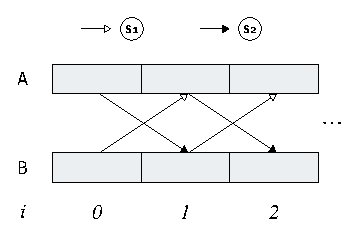
\includegraphics[width=\textwidth,keepaspectratio]{fig_loop-carry}}
\end{minipage}
\captionof{lstlisting}[Loop-carried dependence]{
Loop-carried dependence.
After the first iteration, in every iteration \pr|S2| uses a value of array \pr|A| computed in the previous iteration by \pr|S1|.
Similarly, \pr|S1| uses a value of array \pr|B| computed in the previous iteration by \pr|S2|.
There is a true dependence from \pr|S2| to \pr|S1| and from \pr|S1| to \pr|S2|, and both dependencies are carried by the loop.
If we select any individual iteration and execute it alone, no dependence exists.
}\label{lst:loop-carried}
\end{center}

If loop statements depend only on statements in the {same iteration}, then there exists a loop-independent dependence.
A \emph{loop-independent dependence}~\cite[p. 76]{kennedy2001} occurs when
\pr|S1| references a location \pr|X| on iteration \(i\),
\pr|S2| references \pr|X| on iteration \(i\),
and there is a control flow path from \pr|S1| to \pr|S2|.

Comparing the two loop dependencies, a loop-carried dependence determines the iteration order and whether that order can be transformed safely.
A loop-independent dependence determines the statement execution order within a nest of loops.

\paragraph*{Dependence analysis.}
Detecting dependencies is the focus of dependence analysis\index{dependence analysis}.
\emph{Dependence analysis} (or a \emph{dependence test})
is a technique for identifying or characterizing program dependencies and dependence-preserving reorderings;
which then may permit transformation or parallel execution.
Among the well-established approaches are
the Banerjee test~\cite{banerjee1997}\index{Banerjee test},
GCD test~\cite{zima199}\index{GCD test},
Omega test~\cite{pugh1991}\index{Omega test},
and commutativity analysis~\cite{rinard1996}\index{commutativity analysis}.
We defer further discussion to~\autoref{sec:vmcai}, that presents a dependence analysis inspired by implicit computational complexity.

\subsubsection{Incorporating Parallelism}

If we only focus on sequential code, the notions around dependence are well-established.
However, sequential reasoning is insufficient for effective use the parallelism that is available in modern processors.
Developing and designing parallel software and algorithms is conceptually challenging.
One of the major difficulties is the effort required to ensure that a parallel program is (functionally) correct.
In addition to all the errors that arise in sequential programs, parallelism introduces a new class of bugs that includes race conditions.
A race condition is devious because the runtime behavior of a program with such a bug is nondeterministic~\cite[p. 32]{chapman2007}.
But in exchange for the challenge, parallelism provides the potential to improve the program's runtime performance.
In practice, exploiting parallelism is necessary for all performance-critical applications~\cite{suomela2022}.

There are several good motivations for introducing parallelism in programs and for improving the existing parallelization techniques.
High-performance multicore processors are ubiquitous and possess the abilities to execute several operations in a single clock cycle.
Due to physics, improvements in hardware design now come from parallel processing capabilities, rather than adjustments in clock cycles.
On the software side, a vast majority of legacy applications, and the algorithms that power them, were developed without parallelization in mind.
\emph{Parallelizing compilers}, that automatically translate sequential programs to multicore executables, have made big advances toward improving prevalence of parallelism.
But despite the advances, these compilers make conservative choices and miss opportunities to parallelize~\cite{holewinski2012}.
Correct and efficient parallel code is thus often hand-crafted in a process that is time-consuming and error-prone.

Ultimately, our abilities to parallelize programs relies on the potential parallelism available in the program and the processor;
and the degree to which we can extract parallelism from a sequential program and find the best parallel schedule under the processor's scheduling constraints~\cite{alfred2007}.
No parallelization strategy fits all cases and it is important to facilitate the discovery of new strategies and parallel algorithms as complementary to existing techniques.
For example, running automatic analysis on a large application can distinguish regions that can be parallelized automatically from those that need manual changes.

\paragraph*{From dependence to independence.}
Since dependence determines how program executions may be reordered, it provides a strong foundation for developing techniques to increase the parallelism available in programs.
Parallelism inherently requires \emph{independence} between statements;
in other words, we are interested in absence of dependence.
Thus, if we can design algorithms, or transform programs in ways that increase prevalence of independent statements, we improve the program's parallelization potential.
One focus area in parallelization concerns \emph{loop-level parallelism} that aims is to extract parallel tasks from loops.
For example, by the Loop Parallelization Theorem, it is permissible to convert a sequential loop to a parallel one if the loop carries no dependence~\cite[p. 82]{kennedy2001}.
The remainder of this section focuses precisely on the terms and techniques of parallelizing loops.

\paragraph*{Parallel programming models.}
Multiple sophisticated programming models exist to simplify the task of writing parallel programs.
These models raise the abstraction level between the application code and the operating system-level parallelization mechanism of threading.
The OpenMP\index{OpenMP}\index{parallel programming model!OpenMP}
application programming interface is presented in~\autoref{openmp}.
Other approaches include the
\emph{Parallel Patterns Library} (PPL)\index{PPL}\index{parallel programming model!PPL}~\cite{ppl2021,campbell2011},
that parallelizes tasks through built-in algorithms and containerization;
and the \emph{oneAPI Threading Building Blocks} (oneTBB)\index{oneTBB}\index{parallel programming model!oneTBB},
a runtime-based model for \pr|C++|\index{C++} programs~\cite{onetbb}.

\subsubsection{The OpenMP Programming Model}
\label{openmp}

{OpenMP}\index{OpenMP}\index{parallel programming model!OpenMP}, for Open Multi-Processing,
is a parallel programming model for developing portable, shared memory\index{shared memory} parallel applications in
\pr|C|\index{C},
\pr|C++|\index{C++} and
\pr|Fortran|\index{Fortran}\index{programming language!Fortran}~\cite{openmp_api}.
OpenMP is not a programming language;
rather, it provides directives for sequential programs that translate the programs to parallel execution instructions at compile-time.
The OpenMP\index{OpenMP} infrastructure includes compiler directives, library routines, environment variables, and tool support for creating, debugging, and analyzing parallel applications.

Program execution in OpenMP follows the \emph{fork-join programming model}~\cite[p. 24]{chapman2007}\index{fork-join programming model} of~\autoref{fig:fork-join}.
Program execution starts with an {primary thread}\index{primary thread}
%\footnote{Color \tikz\draw[pthread,fill=pthread] (0,0) circle (.5ex); is the primary thread in drawings.}
that runs in sequential mode.
After encountering a specially-marked parallelizable program region, the primary thread spawns a team of threads in a \emph{fork}\index{fork}-operation.
The team collaborates to complete the tasks of the parallel program region.
The execution concludes with a \emph{join}\index{join}-operation, where the forked threads terminate.
The primary thread\index{primary thread} continues execution past the parallel program region\index{parallel region}, running again in sequential mode.

\begin{figure}[H]
\centering
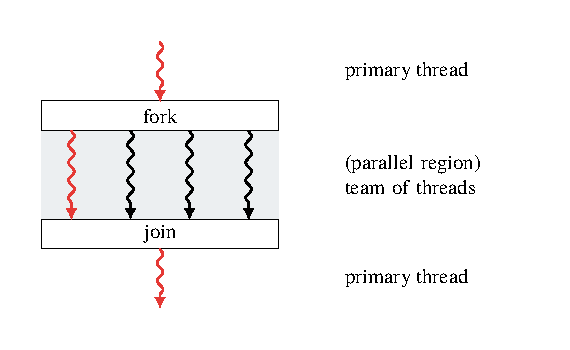
\includegraphics{fig_fork-join}
\caption{The fork-join programming model.}
\label{fig:fork-join}
\end{figure}

In OpenMP, a programmer annotates {structured blocks} with parallelization {directives} to control the parallel execution behavior.
A \emph{structured block}\index{structured block} is a block of executable statements with a single point of entry and exit.
A \emph{parallelization directive}\index{parallelization directive} is a syntactical comment that specifies instructions for how the {structured block}\index{structured block} should be executed.
The syntax and semantics of {parallelization directives}\index{parallelization directive} are defined by OpenMP\index{OpenMP}.
It the responsibility of the programmer to apply the directives safely.
During compilation, an OpenMP\index{OpenMP}-aware compiler translates the directives into parallel-executable instructions~\cite{oak-slides}.
Other compilers a free to ignore the directives.
OpenMP\index{OpenMP} applications are suitable for running on multicore chips, GPUs\index{GPU}, and various other devices attached to a CPU\index{CPU}.
OpenMP is developed and maintained by the OpenMP Architecture Review Board (ARB).

\paragraph*{Foundational terms.}
The following are basic parallel programming terms needed to discuss OpenMP directives~\cite{openmp_api};
refer to \autoref{lst:parallel} for a visual.
A \emph{thread}\index{thread} is a logical {execution entity}, equipped with a stack and associated thread-specific memory.
The threads are identified by numeric ids.
Once a non-empty set of threads is assigned to execute implicit tasks of a parallel region, the {set of threads} becomes a \emph{team}\index{team}.
\emph{Region}\index{region} refers to all {code} encountered during execution, including code encountered in called procedures.
A region is a \emph{parallel region}, if it has an associated set of implicit tasks, and has been assigned a team to execute those tasks.
A \emph{task}\index{task} is a specific instance of {executable code and its data environment} that can be scheduled for execution.
If a task is generated by an implicit parallel region, or through an encounter with a parallel construct during execution, it is an \emph{implicit task}.
Finally, a \emph{barrier}\index{barrier} is a blocking synchronization construct at a program {execution point}.
No thread in a team may execute beyond a barrier until all team members have reached the barrier.

Additional terminology relates to parallelization of loops.
A \emph{worksharing loop}\index{worksharing loop} is a loop-associated construct that satisfies
the worksharing loop property\index{worksharing loop property}.
The \emph{worksharing loop property}\index{worksharing loop property} requires that a construct
distributes the iterations of the associated loops among the threads\index{thread} of the team that encounters the loop~\cite[p. 113]{openmp_api}.

\paragraph*{Essential parallel directives.}
{Parallelization directives}~\index{parallelization directive} are at the core of OpenMP\index{OpenMP}.
This section introduces a few important ones, including the directives that appear elsewhere in this dissertation.
Because OpenMP is a powerful and rich programming model, it is possible to present only a light introduction.
A complete definition is available in the OpenMP API technical specification~\cite{openmp_api}.

\begin{itemize}

\item \texttt{\#}\omp{pragma omp}
is a directive specification in the style of
\pr|C|\index{C}/%
\pr|C++|\index{C++}.
A {parallelization directive}~\index{parallelization directive} must start with these keywords.

\item The \omp{parallel} construct
marks a {structured block}~\index{structured block} parallelizable~\cite[p. 384--385]{openmp_api}.
\autoref{lst:parallel} shows the syntactic use and illustrates its behavior.
When a thread\index{thread} encounters the \pr|parallel| construct,
it forms a {team of threads} to execute the associated {structured block}\index{structured block}.
The structured block becomes a {parallel region}\index{parallel region}.
The thread that encountered the \pr|parallel| construct is the \emph{primary thread}\index{primary thread} of the team.
All threads in the team execute the {parallel region}\index{parallel region}.
An implicit \emph{barrier}\index{barrier} occurs at the end of a {parallel region}\index{parallel region}.
After the parallel region, the {primary thread}\index{primary thread} resumes execution of the enclosing region.

\end{itemize}

\begin{center}
\captionsetup{type=lstlisting}
\begin{minipage}{.45\textwidth}
\ompcodeinputlisting{parallel.c}
\end{minipage}\hfill%
\begin{minipage}{.5\textwidth}
\hfill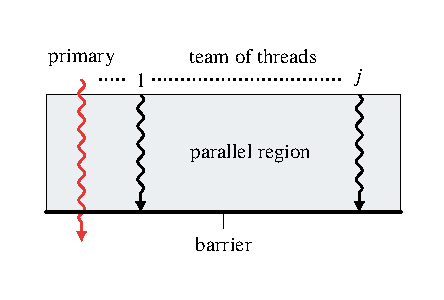
\includegraphics{fig_openmp}
\end{minipage}
\captionof{lstlisting}[The OpenMP \texttt{parallel} construct]{
The OpenMP \pr|parallel| construct and parallel execution with \(j\) threads.%
\index{barrier}\index{thread}\index{parallel region}
}\label{lst:parallel}
\end{center}

\paragraph*{Synchronization constructs.}
Synchronization constructs~\cite[p. 473--482]{openmp_api} enable controlling co-operation of threads\index{thread} over parallel executions.

\begin{itemize}

\item The \omp{atomic} construct ensures a specific memory location is accessed atomically.
It ensures that possible simultaneous reads and writes by multiple threads\index{thread} do not result in indeterminate values.

\item The \omp{barrier} construct specifies an explicit synchronization barrier\index{barrier}.
It prevents any thread\index{thread} from continuing past the barrier until all threads of the sane team encounter the barrier.

\item The \omp{critical} construct means execution of a structured block is restricted to a single thread\index{thread} at a time.

\item The \omp{nowait} clause overrides any synchronization that would otherwise occur at the end of a structured block.
Thus, \omp{nowait} enables specifying that an implicit barrier should not occur.

\end{itemize}

\begin{center}
\begin{minipage}{\textwidth}
One thread\index{thread} executes each iteration sequentially, \(\text{total time} = N \times t_\text{iter}\).
\begin{center}
\captionsetup{type=lstlisting}
\begin{minipage}{.45\textwidth}
\cinputlisting{serial-exec.c}
\end{minipage}\hfill%
\begin{minipage}{.45\textwidth}
\hfill
\includegraphics{fig_exec-seq}
\end{minipage}
\captionof{lstlisting}[Serial execution]{Serial execution.}
\label{lst:serial}
\end{center}
All available threads\index{thread} will execute each iteration sequentially, overwriting values of array \pr|C|, \(\text{total time} = N \times t_\text{iter}\).
\begin{center}
\captionsetup{type=lstlisting}
\begin{minipage}{.45\textwidth}
\ompcodeinputlisting{parallel-loop.c}
\end{minipage}\hfill%
\begin{minipage}{.45\textwidth}
\hfill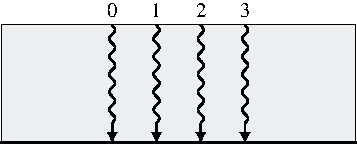
\includegraphics{fig_exec-parallel}
\end{minipage}
\captionof{lstlisting}[Parallel execution]{Parallel execution.\ompi{parallel}\ompi{pragma omp}}
\label{lst:just-parallel}
\end{center}
Assuming a thread\index{thread} count of 4, the threads distribute the loop iteration space uniformly, \(\text{total time} = \frac{N}{4} \times t_\text{iter}\).
\begin{center}
\captionsetup{type=lstlisting}
\begin{minipage}{.45\textwidth}
\ompcodeinputlisting{parallel-for.c}
\end{minipage}\hfill
\begin{minipage}{.45\textwidth}
\hfill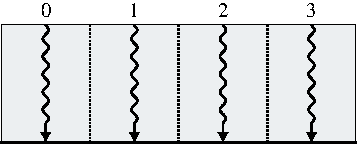
\includegraphics{fig_exec-for}
\end{minipage}
\captionof{lstlisting}[Parallel worksharing]{Parallel worksharing.\ompi{for}\ompi{parallel}\ompi{pragma omp}}
\label{lst:parallel-for}
\end{center}
\captionof{figure}[Parallel worksharing in loop executions]
{The impact of applying parallel worksharing directives to loop executions, adapted from~\textcite{oak-slides}.}
\label{fig:parallel-for}
\end{minipage}
\end{center}

\paragraph*{Work distribution and tasking constructs.}
Parallel executions of structured blocks are controllable by work distribution and tasking directives.
Looping operations on arrays and matrices, like images and tabular data, are often prime candidates for parallelization.
OpenMP has specialized directives to support parallelization of loops.
When applying parallelization directives, the programmer must make sure that the loop is safe to parallelize and performs a sufficient amount of work to benefit from parallelization.

\begin{itemize}

\item The \omp{for} construct is a worksharing loop\index{worksharing loop}.
It specifies that the iterations of associated loop(s) will execute in parallel~\cite[p. 416]{openmp_api}.
The team\index{team} that encounters the loop will perform its execution.
The sequential iteration order is consistent with the execution of the collapsed iterations of a parallel \omp{for} region\index{parallel region}.
The \omp{for} construct supports \eg explicit scheduling, and is compatible with the \omp{nowait} clause.
The \omp{schedule} clause specifies how the loop iterations are divided into chunks and how the chunks are distributed between threads.
The basic use and effect of the \omp{for} construct are demonstrated in~\autoref{fig:parallel-for} and in ~\autoref{lst:parallel-for}.

\item The \omp{loop} construct
supports compiler optimization and parallelization of loops for which logical iterations may execute in any order, including concurrently~\cite[p. 423--424]{openmp_api}.
More precisely, it specifies that the iterations of the associated loop(s) may execute concurrently, in the order specified by an \omp{order} clause.
A loop construct is a worksharing construct if and only if its binding region is the innermost enclosing \omp{parallel} region\index{parallel region}.
It is possible to use a shortcut expression \omp{parallel loop}, combining the two constructs, if the construct refers to one or more loops and no other statements.

\item The \omp{single} construct restricts the execution of a structured to one thread\index{thread}~\cite[p. 405]{openmp_api}.
The executing thread is not necessarily the primary thread;
the choice is implementation-specific.
An implicit barrier\index{barrier} concludes a \omp{single} region.

\end{itemize}

\paragraph*{Shared vs. private data.}
In a multi-threaded shared memory environment, it is necessary to specify how variables are accessed by the executing threads\index{thread}.
This behavior can be controlled with the data-sharing attribute clauses~\cite[p. 224--225]{openmp_api} that are a kind of data environment modifiers.
Both clauses presented here take as a parameter a list of variables names or procedure pointers.
The use of data-sharing attribute clauses is demonstrated in~\autoref{lst:para-block}.

\begin{itemize}

\item The \omp{private} clause privatizes the variables in the parameter list.
It creates a new variable for each variable in the parameter list, and for each thread\index{thread} executing the parallel region\index{parallel region}.
Thus, each thread has its a thread-specific variable copy.
A private variable is uninitialized.

\item The \omp{shared} clause declares that the variables appearing in the parameter list will be shared across the threads\index{thread} executing the parallel region.
The programmer must ensure, with proper synchronization, that the shared memory remains available until execution of the parallel region\index{parallel region} completes.

\end{itemize}

\begin{example}[Parallel transformation]\label{ex:seq-transformation}

We demonstrate a parallelization transformation inspired by~\textcite{singal2019}.
The original sequential code is in~\autoref{lst:seq-block}, where a loop iterates over
fixed-size array length \pr|N|, manipulating each array index in arrays \pr|A| and \pr|B|
(we assume both arrays to be of length \pr|N|).

\begin{center}
\begin{minipage}{\textwidth}
\begin{minipage}{.45\textwidth}
\captionsetup{type=lstlisting}
\cinputlisting{seq-block.c}
\captionof{lstlisting}[Sequential version]{Sequential version.}
\label{lst:seq-block}
\end{minipage}\hfill%
\begin{minipage}{.45\textwidth}
\ompcodeinputlisting{para-block.c}
\captionof{lstlisting}[Parallel version]{Parallel version.\ompi{private}\ompi{shared}\ompi{for}\ompi{parallel}\ompi{pragma omp}}
\label{lst:para-block}
\end{minipage}
\end{minipage}
\end{center}

In~\autoref{lst:para-block}, the loop iteration space is distributed equally between the threads of a team.
Given a team of \(j\) threads, each thread will roughly complete the work of \(N/j\) iterations.
OpenMP often makes the parallelization step straightforward, in this case requiring just one line of directives.
By the data-sharing attribute clauses, the arrays \pr|A| and \pr|B| are explicitly shared across
the threads\index{thread} and the iteration variable \pr|i| is privatized.
\end{example}

\subsubsection{Built-In Loop Transformations in OpenMP}
\label{openmp-transforms}

OpenMP includes built-in directives that perform loop transformations\index{loop transformation}~\cite{openmp_api}.
A loop-transformation replaces the associated loop with a structured block\index{structured block}
that is another loop or a loop sequence.
Unless otherwise specified, all generated loops have canonical form\index{canonical loop}.
Loop-iteration variables of generated loops are always \omp{private} in the innermost enclosing construct.
The loop transformations available in OpenMP are:
fusion\index{loop transformation!fusion},
interchange\index{loop transformation!interchange},
reverse\index{loop transformation!reversal},
split\index{loop transformation!split},
stripe\index{loop transformation!stripe} (interleaving of loop iterations),
tile\index{loop transformation!tile}, and
unroll\index{loop transformation!unroll}.
As an example, we consider the unrolling transformation.

\paragraph*{Loop unrolling.}\index{loop transformation!unroll}
The \omp{unroll} clause~\cite[p. 381--382]{openmp_api}
transforms the associated loop based on the specification provided in the parallelization directive\index{parallelization directive}.
The \omp{unroll} clause is followed by either \omp{full} or \omp{partial} clause.
The effect of \omp{full} clause is to unroll the associated loop fully.
Full unroll requires that the iteration count of the associated loop is a constant.
\autoref{lst:full-unroll} shows the application of the directive and the loop post-transformation form is shown in~\autoref{lst:post-full-unroll}.

\begin{center}
\begin{minipage}{\textwidth}
\captionsetup{type=lstlisting}
\begin{minipage}{.45\textwidth}
\ompcodeinputlisting{full-unroll.c}
\captionof{lstlisting}[Applying full unroll]{Applying full unroll.}
\label{lst:full-unroll}
\end{minipage}\hfill%
\begin{minipage}{.45\textwidth}
\cinputlisting{full-unroll-post.c}
\captionof{lstlisting}[Fully transformed loop]{Fully transformed loop.}
\label{lst:post-full-unroll}
\end{minipage}
\end{minipage}
\end{center}

The \omp{partial} clause takes an integer-valued \emph{unroll factor}\index{unroll factor}.
The effect of \omp{partial} clause is to tile the loop, using the unroll factor as the tile size.
Then, the generated tile\index{loop transformation!tile} loop is fully unrolled.
If no unroll factor\index{unroll factor} is specified, the unroll behavior depends on the implementation.
Partial transformation is illustrated in \autoref{lst:pt-unroll} and~\autoref{lst:post-pt-unroll}.

\begin{center}
\begin{minipage}{\textwidth}
\captionsetup{type=lstlisting}
\begin{minipage}{.45\textwidth}
\ompcodeinputlisting{pt-unroll.c}
\captionof{lstlisting}[Applying partial unroll]{Applying partial unroll.}
\label{lst:pt-unroll}
\end{minipage}\hfill%
\begin{minipage}{.45\textwidth}
\cinputlisting{pt-unroll-post.c}
\captionof{lstlisting}[Partially transformed loop]{Partially transformed loop.}
\label{lst:post-pt-unroll}
\end{minipage}
\end{minipage}
\end{center}

Applying loop transformations\index{loop transformation} requires suitable loop form.
For example, the worksharing loop expects loops to be in canonical form\index{canonical loop}.
Afterward, a transformation that increases the program's parallelization potential\index{parallelization potential} enables making use of multicore hardware during execution.
Thus, an important challenge of parallelizing compilers and program optimizations is to find generalized strategies to increase parallelization potential.

\subsubsection{Implicit Computational Complexity for Parallel Transformations}
\label{icc-fission}

Since implicit computational complexity has developed many systems for reasoning about loops, it seems natural that in extended use, it has potential to support loop-based program transformations.
Founded on this concept,~\autoref{sec:vmcai} presents an ICC-based technique to increase parallelization potential in imperative programs.
The technique uses a static data dependence analysis that detects independent blocks of commands inside loops.
Through a loop fission\index{loop transformation!fission} transformation,
then independent blocks are then transformed into multiple parallelizable loops, as illustrated in~\autoref{fig:icc-fission}.

\begin{figure}[h]
{\centering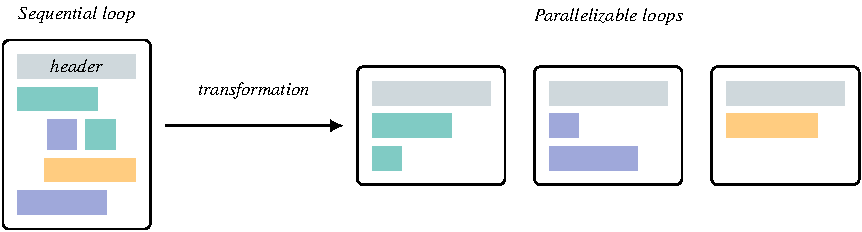
\includegraphics[width=\textwidth,keepaspectratio]{fig_parallel}}
\caption[Loop fission transformation]
{Loop fission of a sequential loop into parallelizable loops.
The loop header (the leading \langclr{header} block) is replicated across the generated loops.
Each generated loop takes a part of the original loop's body.}\label{fig:icc-fission}
\end{figure}

The technique is interesting because it is applicable even when the loop iteration space is unknown;
enabling parallelization of \eg \pr|while| loops.
Such non-canonical loops are traditionally outside the built-in transformation and parallelization capabilities of parallel programming models like OpenMP\@.
Although the \emph{iterations} of \pr|while| loops must be executed under the \omp{single} construct,
the \emph{multiple loops} generated by the transformation can be parallelized with OpenMP directives.
The technique is useful as a preprocessor, before adding parallelization directives;
and in conjunction with other loop transformations.
The technique is inspired by~\cite{moyen20172}, but was adjusted significantly to support the different application.


\subsection{Literature Topic 5: Confidentiality and Non-Interference}\label{pl-sec}
%! suppress = LabelConvention
Computer security is a broad, interdisciplinary field with technical and non-technical challenges.
An important subset of the technical aspects can be modeled and studied mathematically~\cite{piessens2024}.
At its core, computer security is concerned with three properties:
confidentiality\index{confidentiality}, integrity\index{integrity}, and availability\index{availability}.
Although the precise meaning of these terms is situational, they are generally described as follows~\cite[p. 4--6]{bishop2003}.

\begin{description}
\item[Confidentiality]\index{confidentiality}
is about concealment of protected assets, like secret information and resources.
The goal of confidentiality is to ensure protected assets are viewed by authorized users only.
By extension, it includes concealing knowledge about the existence of protected assets.
Confidentiality is compromised if secrets are exposed, or \enquote{leak}\index{leak}, to unauthorized users.

\item[Integrity]\index{integrity}
is about trustworthiness of information and resources.
It aims to ensure protected assets are modified by authorized users only and that those modifications preserve authenticity of the resource.
For example, an update to a date field should yield a legitimate date.
Integrity is difficult to guarantee because it concerns assets over mutations, transmissions, and time.
Authentication\index{authentication} is a critical (though an insufficient) mechanism for enforcing integrity.
Integrity is often considered the dual of {confidentiality\index{confidentiality}}~\cite{biba1977}.

\item[Availability]\index{availability}
refers to the ability to access and use authorized system and its assets.
Availability is compromised if a computational system is unusable or incapable of supporting its intended use;
to include unavailability due to excessive service latency.

\end{description}
The challenge of computer security is to find the right balance between the three;
preventing unauthorized views and modifications, while preserving access and supporting authorized use.
Among the strategies are designing techniques to prevent improper use, detect issues, and recover from compromised scenarios.
Although all three properties are important, the rest of this presentation focuses on confidentiality\index{confidentiality}.

Confidentiality\index{confidentiality} can be enforced with numerous mechanisms, \eg firewalls, access control, and encryption.
A firewall\index{firewall} is a network-layer protection and an operating system implements and maintains access control\index{access control}.
Encryption\index{encryption} protects secret information until decryption\index{decryption}, but its excessive use is problematic for availability\index{availability}.
In general, those mechanisms are insufficient to provide end-to-end guarantees through all layers of computation.
One problem is that confidentiality\index{confidentiality} is not guaranteed after secret information is released as input to a program~\cite{zdancewic2004}.
Information flow\index{information flow} security is concerned with achieving fine-grained confidentiality\index{confidentiality} (and integrity\index{integrity}) guarantees by tracking propagation of information including during program executions~\cite{hedin2012,eggert2014}.

\subsubsection{Information Flow Security}\label{if-security}

Protected assets may require different levels of confidentiality\index{confidentiality}.
Computer systems protecting such assets naturally need controlled information flow\index{information flow}.
The capability to process assets at different security levels is called {\emph{multilevel security} (MLS)\index{multilevel security}}~\cite{bossi2005}.
Illustrated in~\autoref{fig:us-docs}, the United States federal government document classification scheme~\cite{wiki_us_docs} is an example of a multilevel security system.
The permissions cascade: having access to a specific level grants access to all the levels below it.
For example, accessing documents marked \enquote{secret} requires secret or top secret level permission.

\begin{figure}[t]
\centering
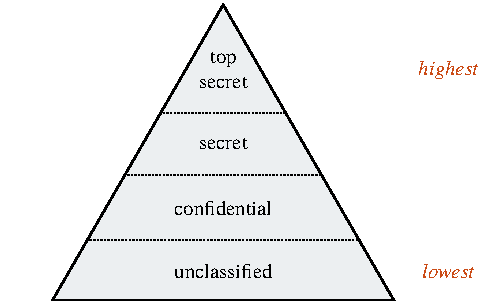
\includegraphics[]{fig_info-flow}
\caption[Document classification scheme]
{The United States federal government document classification scheme.}
\label{fig:us-docs}
\end{figure}


The main idea for achieving secure multilevel information flow is to impose constraints on how privileged information is permitted to flow within the system.
Secure information flow\index{information flow} is a confidentiality\index{confidentiality} guarantee, as it aims to ensure secrets do not leak\index{leak} to unauthorized parties~\cite{piessens2024}.
Implementing secure information flow requires three steps~\cite{eggert2014}.

\begin{enumerate} 

\item Identifying \emph{security classes}\index{security class} (alternatively, domains or user groups).
In~\autoref{fig:us-docs}, the classes are top secret, unclassified, secret, and confidential.

\item Defining a confidentiality \emph{policy}\index{information flow!policy}.
The policy specifies how information is permitted to flow between the security classes.
In~\autoref{fig:us-docs}, the the directed arrows define the policy.

\item Instrumenting an \emph{control}\index{information flow!control}. 
A control is a mechanism that enforces the behavior permitted by the policy.
In~\autoref{fig:us-docs}, no control is specified.

\end{enumerate}

For strong confidentiality\index{confidentiality} guarantees, the information flow approach should also consider and protect against side channels.
\emph{Side channels}\index{side channel} are all system characteristics that enable a malicious actor to deduce secrets,
indirectly and without assistance from other users~\cite[p. 280]{bishop2003}.
In terms of program executions, a few examples of side channels are termination, divergence, deadlocking, and execution latency.
 
\subsubsection{The Elements of Information Flow}
\label{if-elements}

\begin{description}

\item[Information flow]\index{information flow}
is an observable action between two agents\footnote{
The term \emph{agent} is to emphasize abstraction; an agent could be a human user, computer system, web request, program variable, \etc
} \({A}\) and \({B}\)~\cite{eggert2014}.
If an action performed by \({A}\) is observable to \({B}\),
then there exists an information flow from \({A}\) to \({B}\).
The information flow is \emph{explicit}\index{information flow!explicit} 
if it is directly observable from a single action.
The insecure program in~\autoref{fig:bool-ops} shows an example of direct information flow between \pr|high| and \pr|ret|.
Information flow is \emph{implicit}\index{information flow!implicit} 
when it is not directly observable, but the initial action can be deduced from the sequence of actions that follow.
The insecure program in~\autoref{fig:hi-cond} shows an example of an implicit flow.
The initial value of variable \pr|h| is deducible from the returned value \pr|l|, even though there is no direct flow from \pr|h| to \pr|l|.

\item[Information flow policy] (IFP)\index{information flow!policy}
is a statement of what is, and what is not, permissible between security classes~\cite[p. 9]{bishop2003}.
Since the seminal works on information flow~\cite{biba1977,bell1976}, it has been a convention to model information flow policies with lattices~\cite{denning76}\index{lattice}.
The most simple case considers two security classes, 
typically \enquote{high} and \enquote{low} \(({h}, {l})\) (or trusted and untrusted, secret and public, \etc).
In the simple case, the policy condition is that no information should flow from high to low.~\cite{bossi2005}
Then, showing that such a system is secure requires proving that executions that differ only on secrets are indistinguishable~\cite{piessens2024}.
% Transitive vs intransitive policies see, ~\cite{rushby1992}.
A policy that restricts information flow from a lower security class to a higher security class is called a
{non-interference policy}\index{non-interference}, presented in~\autoref{subsec:ni}.

\item[Information flow control] (IFC)\index{information flow!control}
is a mechanism that enforces a {policy\index{information flow!policy}}~\cite{bishop2003}.
Designing adequately expressive and effective controls is an active topic in security research~\cite{vandermeyden2007,bossi2005,sabelfeld2003}.
Like in static analysis (\cf~\autoref{static-analysis-basics}), designing a sound and complete control for arbitrary programs is impossible.
A sound IFC guarantees to find all policy violations\index{violation} and a precise IFC avoids raising excessive false alarms.
However, an overly restrictive IFC is challenging because it compromises availability\index{availability}.
The challenge of information flow control is more nuanced than classic data-flow analysis of functional properties,
because an IFC must consider a program \wrt policies and multiple executions~\cite{frumin2021}.
Thus, the same program can have multiple judgments depending on the policy.

\item[Declassification]\index{declassification}
refers to controlled release of secret information~\cite{sabelfeld2009}.
Declassification\index{declassification} requires a \emph{downgrading}\index{downgrading} operation;
a mechanisms that permits an elevated security judgement to be lowered.
In other words, information is allowed to flow contrary to the {policy\index{information flow!policy}}~\cite{cecchetti2017}.
Declassification\index{declassification} is necessary to support real world security applications.
For example, after a failed login attempt, an unauthorized user is able to observe the effect of the failure, 
although this is an information leak\index{leak}.
Declassification\index{declassification} is generally not safe~\cite{derakhshan2024}, 
and thus poses a major design challenge to IFCs\index{information flow!control}.
In the context of integrity\index{integrity}, declassification is also called {endorsement\index{endorsement}}~\cite{marion2011}.

\end{description}

\paragraph*{Secure and insecure information flows.}
Figures~\ref{fig:bool-ops}--\ref{fig:hi-cond} show basic examples of insecure and secure information flows\index{information flow}.
Variables \pr|high|, \pr|secret|, and \pr|h| are assumed to be secret and their values should not leak\index{leak} from executions.
The programs are fragments from the {IFSPEC benchmark suite}~\cite{hamann2018}\index{IFSPEC} available at~\cite{ifspec}.
The more advanced benchmarks involve, \eg aliasing, reflection, context sensitivity, and exception handling.

\begin{center}
\captionsetup{type=lstlisting}
\begin{minipage}{.45\textwidth}
\begin{center}\javainputlisting{bool-insecure.java}{Insecure.}\end{center}
\end{minipage}\hfill%
\begin{minipage}{.45\textwidth}
\begin{center}\javainputlisting{bool-secure.java}{Secure.}\end{center}
\end{minipage}
\captionof{lstlisting}[Secure and insecure Boolean operations]{
Boolean Operations. The programs are parametric on a Boolean variable \pr|high|.
In the insecure version, the value of \pr|high| is deducible from the value of \pr|ret|.
}\label{lst:bool-ops}
\end{center}

\begin{center}
\captionsetup{type=lstlisting}
\begin{minipage}{.45\textwidth}
\begin{center}\javainputlisting{array-insecure.java}{Insecure.}\end{center}
\end{minipage}\hfill%
\begin{minipage}{.45\textwidth}
\begin{center}\javainputlisting{array-secure.java}{Secure.}\end{center}
\end{minipage}
\captionof{lstlisting}[Implicit information flow leak in an array]{
Arrays Implicit Leak. The insecure program's output reveals if the value of \pr|secret| is or is not 42.
This leak\index{leak} is small, since it corresponds to 1 bit of information.
However, the secure version reveals nothing about the value of \pr|secret|.}
\label{lst:ni-arrays}
\end{center}

\begin{center}
\captionsetup{type=lstlisting}
\begin{minipage}{.45\textwidth}
\begin{center}\javainputlisting{loop-insecure.java}{Insecure.}\end{center}
\end{minipage}\hfill
\begin{minipage}{.45\textwidth}
\begin{center}\javainputlisting{loop-secure.java}{Secure.}\end{center}
\end{minipage}
\captionof{lstlisting}[High conditional incremental leak]{
High Conditional Incremental Leak.
Through the returned value \pr|l|, the insecure version reveals implicitly\index{information flow!implicit} the value of the secret variable \pr|h|.
Compared to~\autoref{lst:ni-arrays}, the program reveals every value of \pr|h|, so the leak\index{leak} here is more significant.
In the secure version, the value of \pr|h| cannot be deduced by the same reasoning.
However, the secure version is also potentially vulnerable through a side channel\index{side channel},
if the loop execution time is observable to an attacker\index{attacker (adversary)}.}
\label{lst:hi-cond}
\end{center}

\subsubsection{Techniques for Information Flow Modeling and Analysis}
\label{if-techniques}

Information flow\index{information flow} can be modeled in several distinct ways.
One way to categorize these approaches is by how they model systems;
\eg state-based automata, trace-based model\index{trace-based model}, and process algebras~\cite{vandermeyden2007}.
The presentation in this dissertation is only concerned with approaches based on programming languages.
The study of security through programming languages is called 
{\emph{language-based security}\index{language-based security}}~\cite{schneider2001,sabelfeld2003}.
The goal of {language-based security\index{language-based security}} is to use principles of programming languages---semantics, analysis, type systems, rewriting, \etc---to strengthen application security.
However, to offer a point of comparison, we introduce briefly trace-based information flow\index{information flow!trace-based}.
The language-based and trace-based approaches have very little in common~\cite[p. 235]{eggert2014}.

\paragraph*{Language-based information flow.}
Language based security formulates information flow constructs through programming languages.
Program logics and security type systems\index{security type system} are among the common techniques~\cite{frumin2021}.
A security type system aims to guarantee the {security policy\index{information flow!policy}} induced by its {lattice\index{lattice}}~\cite{marion2011}.
Each variable is assigned a {{security type}\index{security type}}, \ie a label that indicates its {security class\index{security class}}.
A satisfactorily secure program must pass a compile-time type check of the security labels.
%Language-based information flow typically handles only the two-level security class hierarchy, 
%and does not address intransitive policies~\cite{vonoheimb2004}.
Sections~\ref{subsec:ni} and ~\ref{sec:anytime} discuss the {language-based\index{language-based security}} information flow in more detail.

\paragraph*{Trace-based information flow.}\index{information flow!trace-based}
The trace-based approach~\cite[p. 24]{eggert2014} models a system with a state machine.
In response to actions, the machine transitions, deterministically or nondeterministically\index{nondeterminism}, from state to state.
A \emph{trace}\index{trace} is a sequence of actions of such a machine~\cite{nelson2020}.
Evaluating secure information flow\index{information flow} over traces is about equivalence relations\index{equivalence relation}, 
or {indistinguishability}\index{indistinguishability}.
For example, for a policy\index{information flow!policy} that requires that secrets should not leak\index{leak} to public, 
two traces must be indistinguishable\index{indistinguishability} from the perspective of a public class (they only differ on secret actions).
Further, executing those traces should produce publicly indistinguishable\index{indistinguishability} final states~\cite{nelson2020}.
Showing that a trace-based system satisfies this security requirements is done by {simulation\index{simulation}}~\cite{piessens2024} 
where the simulation proves the trace equivalence \wrt a policy.

\paragraph*{Formal security analysis.}\index{security analysis}
Establishing that a \enquote{system is secure} demands security analysis.
Rigorous formal security analysis considers the following three aspects.

\begin{enumerate}

\item \emph{System model}\index{system model}: a precise mathematical definition of the system to be secured.

\item \emph{Security objective}\index{security objective} (or properties\index{security property}): 
a specification of system behaviors that are considered secure.

\item \emph{Attack model\index{attack model}} (or threat model\index{threat model}): 
a definition of the class of attacks against which the system should be secure.

\end{enumerate}
The parenthesized terms are included because the literature~\cite{bognar2022, bau2011} varies in exact terminology.
However, the goal of formal security analysis\index{security analysis} is uniform.
For a satisfactory system, a formal analysis must conclude with a proof that shows the system satisfies its security specification under the identified threat.
Designing an adequate system model\index{system model}, 
security objective\index{security objective}, 
and attack model\index{attack model} to formally prove system security is nontrivial~\cite{piessens2024}.

\subsubsection{A Primer on Non-Interference}
\label{subsec:ni}

Non-interference\index{non-interference}
is a foundational family of security policies\index{information flow!policy} and security properties\index{security property}
 that constrains information flow\index{information flow} during computations.
The important idea is that a low(er) security class is not permitted to observe a high(er) security class.
In other words, information flow from high to low security class is not allowed.
%Establishing that a system is non-interfering requires showing that behavior of high security class has no impact on low security class.
%(alternatively, that the low level view is independent of the high level).
Although non-interference\index{non-interference}
 is often described in binary terms, referring to just two security classes\index{security class}, it is applicable to arbitrary security hierarchies\footnote{The policy in \autoref{fig:us-docs} is a 4-class non-interference policy.}.
The primary application of non-interference\index{non-interference} 
is in supporting multilevel security\index{multilevel security} systems~\cite{roscoe1999}.

\paragraph*{Classic non-interference.}
The concept of \emph{non-interference}\index{non-interference} was introduced in 1982 by Joseph Goguen and José Meseguer.
Their seminal paper~\cite{goguen1982} presented the concept (only) informally, as follows.
\begin{quotation}
\noindent One group of users, using a certain set of commands, is non-interfering with another group of users if what the first group does with those commands has no effect on what the second group of users can see.
\end{quotation}
Broadly, the paper provided an early framework for formal modeling and verification of information flow\index{information flow}
over deterministic state machines.
This early view of deterministic non-interference\index{non-interference} is regarded as \emph{classical non-interference}~\cite{focardi1997}.

The terminology around non-interference\index{non-interference} and confidentiality\index{confidentiality} 
is somewhat inconsistent~\cite{sabelfeld2003,vandermeyden2007}.
For example, surveying mathematical formalizations, Nelson et al.~\cite{nelson2020} 
identified four distinct characterizations of non-interference\index{non-interference}.
It therefore more accurate to consider non-interference\index{non-interference} as a family of 
information flow\index{information flow} properties that share the above common core.
Non-interference\index{non-interference} has been studied in in a variety of models, 
\eg {trace-based models\index{trace-based model}},
process calculi, programming languages, probabilistic models, timed models, and {cryptographic protocols\index{cryptography}}~\cite{bossi2005}.
\autoref{sec-types} will present how to formulate non-interference in terms of programming languages.

\paragraph*{Practical challenges with non-interference.}
Non-interference is a strong notion because it includes the absence of both 
explicit\index{information flow!explicit} and implicit\index{information flow!implicit} information flows~\cite{bossi2005}.
As noted by many authors~\cite{cecchetti2017,bossi2005}, the requirement is too strong for practical applications.
Strict non-interference is not achievable in real world systems~\cite{bossi2005}.
The non-interference requirement may also be excessively restrictive when additional knowledge about the system is available~\cite{bossi2005}.
For example, consider two \enquote{high} users communicating over an encrypted channel,
 and a \enquote{low} user who can observe the communication events.
In this case, there is an implicit\index{information flow!implicit} flow about the event, but the exchanged information remains secret.
Such controlled leak may be practically acceptable, but classic non-interference would not permit it.
Declassification\index{declassification} (\cf~\autoref{if-security}) allows controlled and restricted 
information flows\index{information flow} against the non-interference policy\index{information flow!policy}.
It is an important mechanism to support security requirements of real world systems.

Proving that a system satisfies non-interference is harder than proving functional correctness~\cite{frumin2021}.
The reason is that functional correctness is a property of each single program execution.
Non-interference, when expressed with trace-based information flow, is stated over multiple runs of the same program.
A non-interference proof requires showing that for different behaviors of high security class the low security class cannot observe any different behavior~\cite{frumin2021}.
When a program property is expressed over a set of trace properties it is called a {\emph{hyperproperty}\index{hyperproperty}}~\cite{clarkson2010}.
Since a non-interference\index{non-interference} proof requires sets of execution traces, 
{non-interference\index{non-interference}} is a {hyperproperty\index{hyperproperty}}~\cite{mastroeni2019}.

\paragraph*{Extensions.}
The classic definition of {non-interference\index{non-interference}} has been extended in several directions.
The following list contains several variants, though the list is necessarily incomplete.
See~\cite{vandermeyden2010,nelson2020,eggert2014} for comprehensive expositions of {non-interference\index{non-interference}} comparisons of the different varieties.
{Progress-sensitive non-interference\index{non-interference!progress-sensitive}} is consider the gold standard of non-interference based information flow\index{information flow} security~\cite{derakhshan2024}.

\begin{itemize}

\item\emph{Bipartite non-interference}~\cite{aceto2024}\index{non-interference!bipartite}
is defined in terms of two levels, low and high.

\item\emph{Nondeterministic non-interference} (NNI)~\cite{focardi1997}\index{non-interference!nondeterministic}
is a generalization of classic non-interference to nondeterministic systems.

\item\emph{Termination-Insensitive noninterference} (TINI)~\cite{hedin2012}\index{non-interference!termination-insensitive}
requires that terminating executions satisfy non-interference.

\item\emph{Termination-sensitive noninterference} (TSNI)~\cite{hedin2012}\index{non-interference!termination-sensitive}
extends classic non-interference by considering divergence as distinguishable from termination,
requiring that the behavior must be consistent for all executions.

\item\emph{Progress insensitive non-interference} (PINI)~\cite{bay2020}\index{non-interference!progress-insensitive}
generalizes termination-insensitive non-interference to accommodate I/O interactions,
where executions agree stepwise on same observable behaviors, permitting silent divergence.

\item\emph{Progress sensitive non-interference} (PSNI)~\cite{hedin2012}\index{non-interference!progress-sensitive}
demands that executions agree on making stepwise progress and match on the public observables.

\item\emph{Deadlock-sensitive non-interference} (DSNI)~\cite{vandenheuvel2024}\index{non-interference!deadlock-sensitive}
considers deadlocking as an observable behavior,
and requires executions agree on deadlocking behavior.

\item\emph{Intransitive non-interference}~\cite{roscoe1999}\index{non-interference!intransitive}
is a relaxed notion of non-interference, where implicit flows may be permitted.

%\item\emph{Anytime non-interference}~\cite{aubert2025}\index{non-interference!anytime}
%considers stepwise non-interference where a satisfactory program may be interrupted arbitrarily without compromising the guarantee.
%Anytime noninterference is presented in~\autoref{sec:at-soundness}.

\end{itemize}
Finally, a note on \emph{non-leakage}\index{non-leakage} and \emph{non-influence}\index{non-influence}~\cite{vonoheimb2004}.
The terms recur in information flow\index{information flow} literature, \eg~\cite{nelson2020,ileri2024};
and are related to {non-interference\index{non-interference}}, but different.
While non-interference restricts information flow \emph{between} security classes,
{{non-leakage}\index{non-leakage}} is a view-partitioning constraint --
it restricts the \emph{parts of system state} a security class is allowed to infer.
Non-leakage considers the same trace\index{trace} over two states (instead of two traces over same states).
The expectation is that executing the same trace from the two states should result in indistinguishable states~\cite{nelson2020}.
Finally, {{non-influence}\index{non-influence}} is the combination of non-interference (as defined in~\cite{rushby1992}) and non-leakage.

\subsubsection{Non-Interference With Security Types}
\label{sec-types}

In the context of programming languages, a program is {non-interfering\index{non-interference}} if 
{secret (high) inputs} do not affect the calculation of {public (low) outputs}~\cite{sabelfeld2003}.
The idea to use programming languages to model {non-interference\index{non-interference}} was introduced by Volpano, Smith and Irvine~\cite{volpanoI1996}.
The paper shows that {non-interference\index{non-interference}} can be soundly approximated using a {security type system\index{security type system}}.
The influential result has since then been followed by numerous works in language-based security.
Among a few examples, {non-interference\index{non-interference}} has been studied in terms of
static program analysis~\cite{barthe2007,huang2014},
{secure compilation\index{secure compilation}}~\cite{patrignani2017,myers1999,cecchetti2017},
formal methods~\cite{kammuller2008,nelson2020},
program logics~\cite{frumin2021,karbyshev2018,garg2006,beringer2007},
verification~\cite{eilers2023},
and software {testing\index{testing}}~\cite{hritcu2013}.
In general, evaluating {non-interference\index{non-interference}} over at different levels of abstractions
(compilation, instruction set architecture, processor, hardware, digital circuits) is necessary,
because even if a program is {non-interfering\index{non-interference}} \wrt its syntax,
it is not protected against vulnerabilities occurring at lower abstraction levels~\cite{piessens2024}.
To develop intuition of programming languages based {non-interference\index{non-interference}},
the rest of this subsection shows examples using {a security type system\index{security type system}} adapted from~\cite{sabelfeld2003}\footnote{
The system is equivalent to Volpano et al. but more conventional in style.}.

\paragraph*{Programs, non-interference, and typing rules.}
For a programming language, we consider the grammar\index{grammar} shown in ~\autoref{fig:ni-syntax}.
A program (command) in this language is denoted by \pr|C|.
Computation starts in an input state with high and low variables \(s = (s_h, s_l)\).
Either \pr|C| terminates in an output state with final values \(s' = (s_h', s_l')\), or diverges, which we denote by \(\bot\).
Letting \(S\) be the set of input states, \(s \in S \),
%The semantics \(\sem{\text{\pr|C|}}\) map an input state \(s \in S \) either to an output state \(\sem{\text{\pr|C|}}s \in S\) or to divergence.
the semantics \(\sem{\text{\pr|C|}}\) of \pr|C| is defined by a function \(\sem{\text{\pr|C|}} : S \rightarrow S_\bot \) where \( S_\bot = S \cup \{ \bot \} \) and \( \bot \notin S\).
The variation of high input is an equivalence relation\index{equivalence relation} \(=_L\).
Two inputs are equivalent if they agree on low values, \ie \(s =_L s'\) iff \( s_l = s_l' \).
The attacker's\index{attacker (adversary)} observational power is characterized by a relation on behaviors defined by the semantics, denoted \(\approx_L\).
Two behaviors are related by \(\approx_L\) iff they are indistinguishable\index{indistinguishability} to the attacker\index{attacker (adversary)}.
%The relation \(\approx_L\) reflects the low security class viewpoint of the system.
Formally, program \pr|C| is secure \wrt non-interference iff
\begin{align*}
\forall s_1,s_2, \in S \cdot s_1 =_L s_2 \implies \sem{C}_{s_1} \approx_L \sem{C}_{s_2}
\end{align*}
which reads:
\begin{quotation}
\noindent If two input states share the same low values, then the behaviors of the program executed on these states are indistinguishable by the attacker\index{attacker (adversary)}.
\end{quotation}
The security typing rules are shown in~\autoref{fig:ni-types}.
For the typing rules, an expression \(\vdash\prm{e} : \tau\) means \pr|e| has type \(\tau\).
The judgement \(\Gamma\vdash\text{\pr|C|}\) means the program \pr|C| is typable in security context \({\Gamma}\).
Expression types and security contexts can be either low (\({l}\)) or high (\({h}\)).
The symbol \(\Gamma\) refers to the current context (low or high).

\begin{figure}[t]
\centering\begin{align*}
C \, ::={ }& \, \mathbf{skip} \mid
\mathbf{v}\coloneqq{}\mathbf{e} \mid
\nonterm C_{{\mathrm{1}}}  \ottsym{;}  \nonterm C_{{\mathrm{2}}} \mid
\ottkw{if} \, \ottkw{e} \, \ottkw{then} \, \nonterm C_{{\mathrm{1}}} \, \ottkw{else} \, \nonterm C_{{\mathrm{2}}} \mid
\ottkw{while} \, \ottkw{e} \, \ottkw{do} \, \nonterm C
\end{align*}
\caption{Grammar of the non-interference security type system.}\label{fig:ni-syntax}
\end{figure}
\begin{figure}[t]
\centering\drules[E]{$\vdash \prm{e} : \tau$}{expression typing}{High,Low}
\centering\drules[C]{$\Gamma \vdash \text{\pr|C|}$}{command typing}{Skip,AssignOne,AssignTwo,Seq,While,If,Sub}
\caption[Non-interference security type system.]{A non-interference security type system.}\label{fig:ni-types}
\end{figure}

\paragraph*{Derivations.}
Consider the programs in Figures~\ref{lst:bool-ops}--\ref{lst:hi-cond}.
Since the programs are written in Java\index{Java}, the constructs are richer than available in the type system grammar\index{grammar}.
The programs are not fully analyzable.
For example, the {security type system\index{security type system}} does not specify how to handle the array in~\autoref{lst:ni-arrays}.
However, we can analyze sub-programs, like the \pr|while| loops in~\autoref{lst:hi-cond} through a mapping to the grammar.
The following examples show basic non-interference\index{non-interference} derivations.

\begin{example}[Secure high conditional incremental leak]\label{ex:high-cond-sec}
We will analyze the following program fragment.

\begin{center}
\begin{minipage}{\textwidth}
\javainputlisting[][linerange={2-2},numbers=none]{loop-secure.java}
\end{minipage}
\end{center}

We assume \pr|h| is an arbitrarily typed variable---neither low or high---and will analyze both cases.
We map the program to the grammar by substituting \pr|h > 0| with \pr|e|₀ and \pr|h--| with \pr|v:=e|₁\footnote{
We lose detail of the compound assignment, but the loss is acceptable for this example.}
to obtain \pr|while(e$_0$) { v:=e$_1$ }|.

\paragraph*{Case 1:  \pr|e|₀, \pr|v|, and \pr|e|₁ are of type high.}
Since the program is derivable as follows, it is non-interfering.

\begin{center}\begin{prooftree}
\infer0[\textsc{E-High}]{\vdash \prm{e}₀ : \mathbf{h}}
\infer0[\textsc{C-Assign1}]{\mathbf{h} \vdash \prm{v:=e}₁}
\infer2[\textsc{C-While}]{\mathbf{h} \vdash \prm{while(e$_0$) \{ v:=e$_1$ \}}}
\end{prooftree}\end{center}

\paragraph*{Case 2: \pr|e$_0$|, \pr|v|, and \pr|e$_1$| are of type low.}
The program is also derivable in low context, and again, is non-interfering.

\begin{center}\begin{prooftree}
\hypo{\mathbf{h} \notin \text{vars}(\prm{e}₀)}
\infer1[\textsc{E-Low}]{\vdash \prm{e}₀ : \mathbf{l}}
\hypo{\mathbf{h} \notin \text{vars}(\prm{v:=e}₁)}
\infer1[\textsc{E-Low}]{\vdash \prm{v:=e}₁ : \mathbf{l}}
\infer1[\textsc{C-Assign2}]{\mathbf{l} \vdash \prm{v:=e}₁}
\infer2[\textsc{C-While}]{\mathbf{l} \vdash \prm{while(e$_0$) \{ v:=e$_1$ \}}}
\end{prooftree}\end{center}

Intuitively, the program is always non-interfering because it processes only high (secret) values, or low (public) values;
never mixing the two security classes.
\end{example}

\begin{example}[Insecure high conditional incremental leak]\label{ex:high-cond-insecure}
We analyze the following program.
It is labeled insecure in the benchmark suite.

\begin{center}
\begin{minipage}{\textwidth}
\javainputlisting[][linerange={2-2},numbers=none]{loop-insecure.java}
\end{minipage}
\end{center}

The goal of this example is to reveal the assumptions that make it insecure.
Using a similar procedure as in~\autoref{ex:high-cond-sec}, we express the program in the type system grammar as
\begin{center}
\pr|while(e$_0$) { v$_1$:=e$_1$; v$_2$:=e$_2$ }|
\end{center}
To maintain the original information flow\index{information flow} behavior,
expressions  \pr|e|₀, \pr|v|₁,  \pr|e|₁
(\resp \pr|v|₂ and \pr|e|₂) must be typable in the same security class\index{security class}.
We also know from \autoref{ex:high-cond-sec} that without multiple security classes\index{security class},
the program is non-interfering\index{non-interference}.
There are two interesting cases.

\paragraph*{Case 1: \pr|e|₀, \pr|v|₁, \pr|e|₁ are high, and \pr|v|₂, \pr|e|₂ are low.}
The derivation beings as follows.

\begin{center}\begin{prooftree}
\infer0[\textsc{E-High}]{\vdash \prm{e}₀ : \mathbf{h}}
\infer0[\textsc{C-Assign1}]{\mathbf{h} \vdash \prm{v}₁\prm{:=e}₁}
\infer0[]{\text{\circled[red]{\normalfont{\textbf{\texttt{X}}}}} \vdash \prm{v}₂\prm{:=e}₂}
\infer2[\textsc{C-Seq}]{\mathbf{h} \vdash \prm{v$_1$:=e$_1$; v$_2$:=e$_2$}}
\infer2[\textsc{C-While}]{\mathbf{h} \vdash \prm{while(e$_0$) \{ v$_1$:=e$_1$; v$_2$:=e$_2$ \}}}
\end{prooftree}\end{center}

Since \pr|v|₂ is of type low, there is no way to handle \pr|v|₂\pr|:=e|₂.
The derivation gets stuck at point marked{ }{ }{\circled[red]{\textbf{\texttt{X}}}}{ }because the program has a non-interference\index{non-interference} violation.
Intuitively, it is because the program operates on a low variable inside a loop with a guard variable\index{guard variable} that is of type high.
This construction is not safe because it leaks information.

\paragraph*{Case: \pr|e|₀, \pr|v|₁, \pr|e|₁ are low and \pr|v|₂, \pr|e|₂ are of type high.}

\begin{center}\begin{prooftree}
\hypo{\mathbf{h} \notin \text{vars}(\prm{e}₀)}
\infer1[\textsc{E-Low}]{\vdash \prm{e}₀ : \mathbf{l}}
\hypo{\mathbf{h} \notin \text{vars}(\prm{e}₁)}
\infer1[\textsc{E-Low}]{\vdash \prm{e}₁ : \mathbf{l}}
\infer1[\textsc{C-Assign2}]{\mathbf{l} \vdash \prm{v}₁\prm{:=e}₁}
\infer0[\textsc{C-Assign1}]{\mathsf{h} \vdash \prm{v}₂\prm{:=e}₂}
\infer1[\textsc{C-Sub}]{\mathsf{l} \vdash \prm{v}₂\prm{:=e}₂}
\infer2[\textsc{C-Seq}]{\mathbf{l} \vdash
\prm{v}_\prm{1}\prm{:=e}_\prm{1}\prm{;}\prm{v}₂\prm{:=e}₂}
\infer2[\textsc{C-While}]{\mathbf{l} \vdash\prm{while(e$_0$) \{ v$_1$:=e$_1$; v$_2$:=e$_2$ \}}}
\end{prooftree}\end{center}

Reversing the security label configuration makes the program typable.
A critical rule is \textsc{C-Sub} (subsumption) that permits lowering the security class label of a high command.
Unlike in the previous case, the loop guard\index{guard variable} is now low type.
It permits manipulating a variable of high type inside the loop body.
\end{example}

\subsubsection{Security Meets Implicit Computational Complexity}
\label{icc-sec}

With a common focus on restrictions, it seems intuitive that 
techniques from implicit computational complexity would pair elegantly with information flow and applications in language-based security\index{language-based security}.
The combination can potentially provide two types of correctness guarantees, relating resource analysis and security.
Supporting this hypothesis, there are already multiple series of work exploring connections between the two domains.
This section gives a brief summary of those results.

\paragraph*{Complexity via non-interference: SAFE programs.}
The class of SAFE programs\index{SAFE programs} is foundational in demonstrating that non-interference security type systems\index{security type system}
can support implicit characterizations of complexity classes.
The idea was introduced by Jean-Yves Marion in~\cite{marion2011}.
SAFE programs continue to be actively investigated by Marion, Emmanuel Hainry, Romain Péchoux, and others.

Starting with the principle of {\emph{tiering}\index{tiering}}\footnote{
The intuition behind tiering, \aka ramification\index{ramification}, is that program execution time depends on the nature of information flow during executions.
The flow can be constrained by imposing a precedence relation that regulates the information flow,
\eg from higher tier to lower tier~\cite{leivant1995, leivant2013}.},
Marion extended the principle to characterize the class of {polynomial time computable functions\index{complexity class!P}}.
A critical step in obtaining this result was combining tiering with a type system\index{security type system} 
for secure information flow\index{information flow}.
Each variable is assigned a type -- a {tier} of either 0 or 1 -- representing elements of a complexity lattice\index{lattice}.
The paper then shows that terminating and well-typed programs are computable in polynomial time.
SAFE programs\index{SAFE programs} is precisely the class of programs captured by this characterization.

Judging by the number of works that followed, the technique was inspirational.
The subsequent results have provided extensions mainly along two directions.
The first has focused on programming language paradigms, including: 
concurrent fork-join processes (SAFE processes\index{SAFE programs!process})~\cite{hainry2013},
dynamic data structure (ramified programs)\index{ramified programs}~\cite{leivant2013}, and
{object-oriented (OO) programs\index{SAFE programs!object-oriented}}~\cite{hainry2015}.
The OOP result is the first characterization of polynomial time\index{complexity class!P} computable functions in the object oriented paradigm.
The second directions has focused on redefining the system restrictions, with the goal of improving intensional completeness\index{completeness}.
For example, the class of stratified programs\index{stratified programs}~\cite{hainry2023} characterizes a strictly larger class than SAFE programs,
by using a combination of {security type system\index{security type system}}, heap memory restriction, and shape analysis\index{shape analysis}.
With the same end-goal, aperiodic programs (AP)~\cite{hainry2024}\index{aperiodic programs} extends SAFE programs by using declassification\index{declassification};
another mechanism adopted from the security domain.
In the latter, the main result is a proof that SAFE and terminating aperiodic programs is the class of Basic Feasible Functionals\index{Basic Feasible Functionals}, \ie \(\sem{\text{SAFE}\;\cap\;\text{AP}\;\cap\;\text{terminating} = \text{BFF}}\)~\cite{hainry2020,hainry2024}.

\paragraph*{From complexity to cryptography.}\index{cryptography}
In opposite direction, a separate track of works uses implicit computation complexity for applications in the security domain.
The formalization of safe recursion (\cf~\autoref{safe-rec}) was primarily motivated by its envisioned utility in cryptography~\cite{heraud2011}.
The type system d\(\ell\)T~\cite{baillot2015,baillot2019}\index{d\(\ell\)T} is simultaneously complexity-aware, and has capabilities to support cryptographic proofs.
%The system over-approximates the complexity of typable programs.
Among the applications, d\(\ell\)T allows proving that the constructed adversary for the Goldreich-Levin Theorem\index{Goldreich-Levin Theorem} is polynomial time\ccxi{p}.
Such applications are interesting because they involve computations that are inherently non-polynomial in time complexity.
Handing such sub-computations %that are non-polynomial time
requires pushing ICC techniques beyond their standard capabilities.
%It is still early to judge the long-term impact of system d\(\ell\)T\@;
%among the challenges, it has not been implemented.
Although d\(\ell\)T has not been implemented, together with the formalization of safe recursion, it
%However, d\(\ell\)T and the formalization of safe recursion have
already inspired other mechanized proofs~\cite{barbosa2021,feree2018}.

\subsubsection{From Quasi-Invariant Chunks to Non-Interference}
\label{quasi-ni}

Reinforcing the existing connections,~\autoref{sec:anytime} presents a program logic for non-interference\index{non-interference} inspired by implicit computational complexity.
The motivating idea was to explore utility and power of ICC techniques in language-based security\index{language-based security} analysis.
The logic analyzes information flows\index{information flow} in imperative programs and abstracts the flow patterns into matrices.
As a technique, it is a refinement of prior works (refer to~\autoref{app:sec:vmcai} and~\cite{moyen20172}) where it was used for compile-time program optimization.
Although the logic no longer enforces complexity bounds, it demonstrates the utility of interchanging techniques between the ICC and security.
Adjusting the logic to track {non-interference\index{non-interference}} revealed various mathematical insights;
for example, that treatment of loops is more straightforward for {non-interference\index{non-interference}} than it is in {complexity analysis\index{complexity analysis}}.
Further, as a data flow analysis\index{dependency analysis} for tracking different program properties, 
it is reminiscent of the {Dependency Core Calculus (DCC)\index{Dependency Core Calculus}}~\cite{abadi1999b}.
The multiplicity of the program logic suggests it has representational capabilities similar to DCC.


\subsection{Literature Topic 6: Formal Verification}\label{verification}
The size and complexity of modern software makes it almost impossible to avoid implementation errors.
Asynchronous computation, the rich array of computing environments and their communication;
and constant modifications are among the challenges that can lead to software \enquote{going wrong}.
Prominent and costly examples include
the Ariane 5 rocket failure an explosion on its maiden flight~\cite{ariane5},
the Therac-25 radiation therapy machine with six instances of lethal overdoses~\cite{leveson1993};
and the loss of NASA's Mars Climate Orbiter~\cite{mars1999}.
In more recent memory, the CrowdStrike incident caused multiple days of system outages
 across critical infrastructure like airports, banks, and hospitals~\cite{crowdstrike}.
In a case involving the~\textcite{usg2024},
a software-related failure exposed sensitive personal information of USG employees with potential harm to the Augusta University community.

Unreliability of software is not isolated to these few publicized instances.
A pithy comment in~\textcite[p. 3]{dijkstra1970} captures a similar sentiment.

\begin{quotation}
\noindent{}Present-day computers are amazing pieces of equipment,
but most amazing of all are the uncertain grounds on account of which we attach any validity to their output.
\end{quotation}

The context of Dijkstra's statement is modest compared to exploding rockets;
it refers to a multiplication operation of two 27-bit integers.
Checking that the machine actually performs the correct operation for all inputs---\ie meets its \emph{specification}---,
at a rate of few microseconds per input-pair, would require more than 10,000 years.
Thus, among computer scientists, the skepticism around software correctness is a long-held position.
It is also the core problem tackled by formal methods.

\paragraph*{Motivations and challanges.}
Formal methods aims to remove uncertainty by providing techniques that allow establishing strong behavioral guarantees.
Formal methods is deeply rooted in mathematics and logic~\cite{shankar2023}.
In this view, programs are defined as precise mathematical \emph{models} with {specifications}.
The specification defines what behavior is expected from the model under study.
Formally \emph{verifying} a program involves constructing a \emph{proof} that the model satisfies its specification.
In contrast to manual inspection and tests (like the one of inspecting every input-pair),
a proof conclusively ensures correctness for all inputs at the model's level of abstraction.
As noted later by~\textcite{dijkstra1972}, \enquote{{[t]he only effective way to raise the confidence level of a program significantly is to give a convincing proof of its correctness.}}

The motivation for using formal methods is based on the strength of guarantees it provides.
Being formal helps when you want to be precise~\cite{leino2023}.
However, thinking formally requires a different engineering mindset.
Instead of thinking of all possible scenarios and how they might go wrong, formal reasoning requires defining how a system is \emph{expected} to work, and identifying conditions that must be met to ensure the correct behavior~\cite{aws2024}.
Those conditions are then formally verified using proofs.

Despite the clear benefits, wider adoption of formal methods is impeded by challenges involving \eg resource investment (formal proofs are time-consuming), tooling, and education~\cite{beek2024}.
A slightly different challenge concerns the \emph{methods} themselves.
The Four Color theorem is the first famous result with a proof that requires large computer calculations.
When the proof appeared in 2008, such proofs were still controversial.
The basis of the controversy was that computer programs could not be reviewed with mathematical rigor~\cite{gonthier2008}.
Thus, a critical factor in advancing formal methods concerns educating wider communities about the capabilities.

\begin{quotation}
\noindent{}We can envision [\ldots] a world in which computer programs are always the most reliable components of any system or device~\cite{hoare2021}.
\end{quotation}

\subsubsection{Foundational Concepts}
\label{subsubsec:verification-concepts}

\paragraph*{Models and specifications.}
A formal \emph{model} is an abstract description of a computer system of interest, expressed in (some) formal modelling language,
and used for reasoning about the system and consequences of design choices~\cite{zave2023,olveczky2017}.
In this dissertation, we are interested in systems that are programs.
In choosing a modeling formalism, it should enable expressing the model as naturally and intuitively as possible,
while still generating mathematically precise structures~\cite{olveczky2017,beek2024}.
In other words, the formalism should omit unnecessary technicalities;
enable focusing on the problem of interest at an appropriate level of abstraction,
and facilitate analysis and reasoning about the program~\cite{olveczky2017}.

The \emph{specification} is a part of the formal model that describes the \emph{behavior} of the program~\cite{zave2023b}.
The specification should be simpler and easier to comprehend than an actual implementation~\cite{zave2023b}.
Critically, we want the specification to be \emph{separate} from the implementation~\cite{furia2014b}.
Such independence enables isolating the mathematical properties of interest and showing that the implementation is consistent with those properties\footnote{
Otherwise, we run into the \emph{Assertion Inference Paradox}:
\enquote{if the specification is inferred from the implementation, what do we prove?}~\cite{furia2014b}}.
The specification should precede the implementation or minimally be developed concurrently~\cite{dijkstra1972}.

One standard way to notate specifications is through Hoare triples~\cite{hoare1969}.
In this view, we consider \(S\) to be some executable statement (a program).
We then define a \emph{precondition} \(P\) that describes conditions that hold before execution,
and a \emph{postcondition} \(Q\) that describes conditions that hold after execution.
Then, a \emph{Hoare triple} is a predicate that connects the statement with the pre- and postconditions by \(\{P\} S \{Q\}\).
Such expression essentially means, starting from \(P\), statement \(S\) will not crash and terminates in a state satisfying \(Q\).
For example, \(\{ \prm{x}=0 \}\;\prm{x++}\;\{ \prm{x}=1\}\) is a valid Hoare triple, which is also provable (though \emph{how} to prove it is a topic for later).

\paragraph*{Invariants.}
Proving that an implementation meets its specification requires more information than what is available in the program syntax~\cite{chang2005}.
For example, to prove a Hoare triple of a loop command often requires establishing additional verification conditions called invariants.
An \emph{invariant}, in programming terms, is an assertion that is preserved by the program execution~\cite{furia2014}.
An invariant is \emph{inductive},
if it holds the first time a program location is reached and is preserved in every cycle returning to that location~\cite{sankaranarayanan2004}.
There are many kinds of invariants, \eg object, class, and loop invariants.
Although having invariants is useful for proving programs, discovering them is among the most difficult problems in verification~\cite{dillig2013,yu2023}.

To provide a concrete example, a \emph{loop invariant} is an expression that holds on loop entry and after every loop iteration.
The program of~\autoref{lst:invariant} has two variables, \pr|i| and \pr|n|.

\begin{center}
\begin{minipage}{\textwidth}
\captionsetup{type=lstlisting}
\cstarinputlisting{invariant.c}
\captionof{lstlisting}[Loop inspection for loop invariants]{Loop inspection for loop invariants.}
\label{lst:invariant}
\end{minipage}
\end{center}

At loop entry, the value of \pr|i| is 0.
If the value of \pr|n| is negative, the loop never iterates.
Otherwise, \pr|i| will hold a value between 0 and \pr|n|.
Based on this analysis, the loop invariant is \(0 \leq \prm{i} \leq \prm{n} \vee \prm{n} < 0\).
A postcondition of \pr|i| is \(\prm{i}=0 \vee \prm{i}=\prm{n}\).
A loop invariant is a {weakened} form of its postcondition~\cite{furia2010}.
Therefore, techniques that aim to infer invariants benefit from the availability of postconditions, as investigated in~\autoref{sec:postcond}.

Finally, a brief note about invariants and complexity.
It is possible to infer complexity bounds of numerical loops based on loop invariants as shown by~\textcite{nguyen2017}.
However, the solution relies on dynamic techniques, that are beyond purely static capabilities.

\paragraph*{Safety and liveness properties.}
Formal verification aims to guarantee that certain behavioral attributes, \ie \emph{properties}, hold for a program.
Memory safety\footnote{
\Ie absence of errors related to memory accesses: null-pointer de-referencing, access to un-allocated memory, dangling pointers, out-of-bounds accesses, double free, \etc~\cite{muller2024}},
absence of overflows, termination, data race and deadlock freedom;
secure information flow (cf~\autoref{if-security}), staying within available resource bounds, and worst-case execution time are a few examples of properties.
To show that a program is free of \eg overflows, we express {overflow-freedom} as a specification,
then prove it against the implementation.

There are various different ways of categorizing classes of properties.
\emph{Functional} properties are technical characteristics that contribute to computation of the correct output.
\emph{Non-functional} properties are concerned with quality attributes like security, dependability, reliability, and resource requirements~\cite{terbeek2018}.
Two other frequently-used categorizing terms are safety and liveness.
They come from a paper by~\textcite{lamport1977}, where
a \emph{safety property} is a guarantee that \enquote{something (bad) will not happen},
and \emph{liveness property} ensures (good things) \enquote{must happen}, eventually.
The proof techniques across these safety and liveness properties are different.
Works in this dissertation are primarily concerned with non-functional safety properties.

\paragraph*{Partial and total correctness.}
Broadly, a program is correct if the implementation is consistent with the specification~\cite{furia2014b}.
However, in making assertions about correctness, we need to be more specific.
There are two common notions around correctness that provide more precision: partial and total correctness.
\emph{Partial correctness} means that every terminating execution is correct, however it does not ensure every execution terminates~\cite[p. 64]{leino2023}.
A stronger guarantee follows from total correctness.
A program is \emph{totally correct} if it is partially correct and always terminates~\cite[p. 64]{leino2023}.
Total correctness can be viewed as a combination of safety and liveness properties~\cite{lamport1977}.
There are several strategies for proving termination in some cases, \cf~\autoref{resource-analysis}.
However, a general method that proves termination of all programs cannot exist since termination is undecidable~\cite{turing1936}.
This means it is impossible to show total correctness of all programs\footnote{
Total correctness is not an absolute ideal.
There are many applications where termination is undesirable, like a web server or cardiac pacemaker; but for which we still want formal guarantees.};
but similar to~\autoref{static-analysis-basics},
there is endless opportunity in building increasingly capable program verifiers.

\subsubsection{Tools for Formal Verification}

Formal methods is inherently concerned with \emph{computer-aided} reasoning.
This means there is a strong emphasis on the software tools that support those motivations.
The tools include solvers, theorem provers, model checkers, verifiers, \etc, with each tool category supporting different use cases.
As a formal methods practitioner, it is helpful to maintain a mental map of available tools and their capabilities, like the one in~\autoref{tab:fm-tools}.
Among the tools, interactive theorem proving and verification-aware programming languages are of special interest to this dissertation.

\begin{table}[p!]
\begin{tabularx}{\linewidth}{@{}lX@{}}
\toprule
\multicolumn{2}{@{}l}{\textbf{Automated theorem provers \& solvers}} \\
&
\href{https://alt-ergo.ocamlpro.com}{Alt-Ergo}\index{Alt-Ergo}%
,{ }\href{https://github.com/bitwuzla/bitwuzla}{Bitwuzla}\index{Bitwuzla}%
,{ }\href{https://cvc5.github.io}{cvc5}\index{cvc5}%
,{ }\href{https://www.cyclist-prover.org}{Cyclist}\index{Cyclist}%
,{ }\href{https://github.com/dreal/dreal4}{dReal}\index{dReal}%
,{ }\href{https://wwwlehre.dhbw-stuttgart.de/~sschulz/E/E.html}{E}\index{E}%
,{ }\href{https://gitlab.com/korovin/iprover}{iProver}\index{iProver}%
,{ }\href{https://mathsat.fbk.eu}{MathSAT}\index{MathSAT}%
,{ }\href{https://fmv.jku.at/picosat/}{PicoSAT}\index{PicoSAT}%
,{ }\href{https://github.com/uuverifiers/princess}{Princess}\index{Princess}%
,{ }\href{https://en.wikipedia.org/wiki/Prover9}{Prover9}\index{Prover9}%
,{ }\href{https://satallaxprover.org}{\mbox{Satallax}}\index{Satallax}%
,{ }\href{http://www.spass-prover.org/}{SPASS}\index{SPASS}%
,{ }\href{https://vprover.github.io}{Vampire}\index{Vampire}%
,{ }\href{https://verit.loria.fr}{veriT}\index{veriT}%
,{ }\href{https://yices.csl.sri.com}{Yices}\index{Yices}%
,{ }\href{https://github.com/Z3Prover/z3}{Z3}\index{Z3}%
\\\midrule
\multicolumn{2}{@{}l}{\textbf{Interactive theorem proving}} \\
&
\href{https://github.com/agda/agda}{Agda}\index{Agda}%
,{ }\href{https://github.com/EasyCrypt/easycrypt}{EasyCrypt}\index{EasyCrypt}%
,{ }\href{https://fstar-lang.org/}{F$^{*}$}\index{F$^{*}$}%
,{ }\href{https://hol-light.github.io/}{HOL Light}\index{HOL Light}%
,{ }\href{https://iris-project.org/}{Iris}\index{Iris}%
,{ }\href{https://isabelle.in.tum.de}{Isabelle}\index{Isabelle}%
,{ }\href{https://lean-lang.org/}{Lean}\index{Lean}%
,{ }\href{https://us.metamath.org/}{Metamath}\index{Metamath}%
,{ }\href{https://pvs.csl.sri.com/}{PVS}\index{PVS}%
,{ }\href{https://rocq-prover.org}{Rocq}\index{Rocq}%
,{ }\href{https://github.com/boyland/sasylf}{SASyLF}\index{SASyLF}%
,{ }\href{https://github.com/ggrov/tinker}{Tinker}\index{Tinker}%
\\\midrule
\multicolumn{2}{@{}l}{\textbf{Invariant synthesis}} \\
&
\href{https://github.com/PL-ML/code2inv}{Code2Inv}\index{Code2Inv}%
,{ }\href{https://plse.cs.washington.edu/daikon/}{Daikon}\index{Daikon}%
,{ }\href{https://github.com/dynaroars/dig/tree/dev}{DIG}\index{DIG}%
,{ }\href{https://github.com/freqhorn/freqhorn}{FreqHorn}\index{FreqHorn}%
\\\midrule
\multicolumn{2}{@{}l}{\textbf{Language-based verification \& modelling languages}} \\
&
\href{https://github.com/boogie-org/boogie}{Boogie}\index{Boogie}%
,{ }\href{https://dafny.org}{Dafny}\index{Dafny}%
,{ }\href{https://www.eiffel.org}{Eiffel}\index{Eiffel}%
,{ }\href{https://cs.nyu.edu/~wies/software/grasshopper/}{GRASShopper}\index{GRASShopper}%
,{ }\href{https://kframework.org}{K}\index{K Framework}%
,{ }\href{https://en.wikipedia.org/wiki/Maude_system}{Maude}\index{Maude}%
,{ }\href{https://rebeca-lang.org}{Rebeca}\index{Rebeca}%
,{ }\href{https://en.wikipedia.org/wiki/SPARK_(programming_language)}{SPARK}\index{SPARK}%
,{ }\href{https://en.wikipedia.org/wiki/TLA\%2B}{TLA+}\index{TLA+}%
,{ }\href{https://github.com/utwente-fmt/vercors}{VerCors}\index{VerCors}%
,{ }\href{https://www.pm.inf.ethz.ch/research/viper.html}{Viper}\index{Viper}%
,{ }\href{https://whiley.org}{Whiley}\index{Whiley}%
,{ }\href{https://www.why3.org}{Why3}\index{Why3}%
\\\midrule
\multicolumn{2}{@{}l}{\textbf{Language extensions adding verification features}} \\
&
\href{https://en.wikipedia.org/wiki/ACL2}{ACL2}\index{ACL2}% %(Common LISP),
,{ }\href{https://www.atelierb.eu/en/atelier-b-tools/online-documentation/}{Atelier B}\index{Atelier B}%
,{ }\href{https://github.com/ocaml-gospel/cameleer}{Cameleer}\index{Cameleer}% %(Ocaml),
,{ }\href{https://github.com/flux-rs/flux}{Flux}\index{Flux}% %(Rust),
,{ }\href{https://frama-c.com}{Frama-C}\index{Frama-C}% %(C),
,{ }\href{https://github.com/viperproject/gobra}{Gobra}\index{Gobra}% %(Go),
,{ }\href{https://www.key-project.org/applications/program-verification/}{KeY}\index{KeY}% %(Java),
,{ }\href{https://ucsd-progsys.github.io/liquidhaskell/}{LiquidHaskell}\index{LiquidHaskell}% %(Haskell),
,{ }\href{https://github.com/marcoeilers/nagini}{Nagini}\index{Nagini}% %(Python),
,{ }\href{https://www.openjml.org}{\mbox{OpenJML}}\index{OpenJML}% %(Java),
,{ }\href{https://github.com/viperproject/prusti-dev}{Prusti}\index{Prusti}% %(Rust),
,{ }\href{https://github.com/epfl-lara/stainless}{\mbox{Stainless}}\index{Stainless}% %(Scala),
,{ }\href{https://github.com/verifast/verifast}{VeriFast}\index{VeriFast}% %(C, Rust, Java)
\\\midrule
\multicolumn{2}{@{}l}{\textbf{Linear programming \& optimization}} \\
&
\href{https://github.com/coin-or/Clp}{Clp}\index{Clp}%
,{ }\href{https://en.wikipedia.org/wiki/CPLEX}{CPLEX}\index{CPLEX}%
,{ }\href{https://github.com/COPT-Public/cuPDLP-C}{cuPDLP-C}\index{cuPDLP-C}%
,{ }\href{https://en.wikipedia.org/wiki/GLOP}{Glop}\index{Glop}%
,{ }\href{https://www.gnu.org/software/glpk/}{GLPK}\index{GLPK}%
,{ }\href{https://en.wikipedia.org/wiki/Gurobi_Optimizer}{Gurobi}\index{Gurobi}%
,{ }\href{https://github.com/ERGO-Code/HiGHS}{HiGHS}\index{HiGHS}%
,{ }\href{https://sat4j.org}{Sat4j}\index{Sat4j}%
\\\midrule
\multicolumn{2}{@{}l}{\textbf{Model checking}} \\
&
\href{https://alloytools.org}{Alloy}\index{Alloy}%
,{ }\href{https://github.com/moves-rwth/attestor}{Attestor}\index{Attestor}%
,{ }\href{https://cpachecker.sosy-lab.org}{CPAChecker}\index{CPAChecker}%
,{ }\href{https://github.com/diffblue/cbmc}{CProver}\index{CProver}%
,{ }\href{https://github.com/uuverifiers/eldarica}{Eldarica}\index{eldarica}%
,{ }\href{https://github.com/loonwerks/jkind}{JKind}\index{JKind}%
,{ }\href{https://github.com/nidhugg/nidhugg}{Nidhugg}\index{Nidhugg}%
,{ }\href{https://www.prismmodelchecker.org}{PRISM}\index{PRISM}%
,{ }\href{https://rebeca-lang.org/alltools/RMC}{RMC}\index{RMC}%
,{ }\href{https://sri-csl.github.io/sally/}{Sally}\index{Sally}%
,{ }\href{https://github.com/tlaplus/tlaplus}{TLC}\index{TLC}%
,{ }\href{https://uppaal.org/}{\mbox{UPPAAL}}\index{UPPAAL}%
\\\midrule
\multicolumn{2}{@{}l}{\textbf{Symbolic execution}} \\
& 
\href{https://klee-se.org}{KLEE}\index{KLEE}%
,{ }\href{https://github.com/jburnim/crest}{CREST}\index{CREST}%
,{ }\href{https://github.com/GillianPlatform/Gillian}{Gillian}\index{Gillian}%
,{ }\href{https://github.com/SymbolicPathFinder/jpf-symbc}{Symbolic JPF}\index{Symbolic JPF}
\\
\bottomrule
\caption[Tools for formal methods]{A categorized collection of formal methods tools.}
\label{tab:fm-tools}
\end{tabularx}
\end{table}

One of the main goals of formal methods is to produce mechanized, \ie machine-checked, proofs.
A mechanized proof \enquote{detaches} proof-checking from the activity of crafting the proof.
Only the interface of the program, \ie the statement of the theorem, needs to be reviewed.
The rest is self-checking and deferred to a theorem prover.
This means everyone with sufficient technical abilities can check the proof once a proof exists (provided they trust the theorem prover).
Mechanized proofs are sometimes compared to \emph{paper proofs}, \ie informal proofs written in natural language, whether actually on paper or written in a text editor.
Since paper proof rely solely on the readers abilities to comprehend and confirm the detailed proof steps, mechanized proofs are functionally distinct and provide more rigorous correctness guarantees~\cite{gonthier2008}.

Mechanized proofs are created with theorem provers, of which there are broadly two categories.
An \emph{automatic theorem prover} (ATP) aims to find proofs without assistance from a user.
The proof \emph{search} problem is challenging in general\footnote{\Eg for first-order logic, the problem is NP-complete~\cite{cook1971, levin1973})}, while use cases expect practical efficiency from the solvers.
Prominent ATPs complete bi-annually on solving \href{https://www.tptp.org/}{\enquote{Thousands of Problems for Theorem Provers}} (TPTP problems)~\cite{sutcliffe2024} at the \href{https://tptp.org/CASC/}{CADE ATP System Competition} (CASC) --
the world championship for automated theorem proving~\cite{casc}.
An \emph{interactive theorem prover} (ITP), \aka \emph{proof assistant}, is a programming environment that helps users write mechanized proofs.
Proof assistants vary in underlying logics and proof style.
To provide some metric of comparability, there is a ranking for tracking the formalization extent of 100 well-known mathematical theorems across proof assistants.
As of April 2025, the top 3 proof assistants with highest coverage of the problems are Isabelle (92\%), HOL Light (89\%), and Rocq (79\%)~\cite{hundredtheorems}.
While automatic theorem provers search for proofs of isolated problems and frequently serve as building block of other verification tools,
interactive theorem provers enable large and complex modular proof developments.

Verification-aware programming languages provide a conceptually different approach to machine-checked proofs.
Such languages are particularly well-suited for reasoning about functional correctness of programs.
Verification-aware programming languages have built-in capabilities to express specifications and proofs.
Additionally, they have an associated verifier that checks the proofs during program development;
typically, a background ATP that offers an interaction interface via a programming language~\cite{leino2023}.
One prominent style among the verification-aware languages is \emph{deductive verification},
where the verification process is based on some form of logical inference, i.e., \enquote{deduction}.
The properties to be proven are expressed in a formal specification language, as structured comments, next to the program constructs they relate to~\cite{hahnle2019}.
A deductive verifier them aims at to prove that all possible behaviors of a program satisfy the specification using the available program annotations~\cite{cassez2022}.

The remainder of this section briefly introduces two tools for formal methods:
the (interactive) Rocq theorem prover (\autoref{subsec:rocq}) and the verification-aware programming language Dafny (\autoref{subsec:dafny}).
These tools are relevant for some of the dissertation manuscripts and assumed to be familiar to the reader.

\subsubsection{The Rocq Theorem Prover}
\label{subsec:rocq}

The Rocq theorem prover is an interactive proof assistant for machine-checked formal reasoning.
It provides a rich and flexible environment for various proof developments.
Rocq is a widely-adopted tool in the programming languages research community with applications in formal assurance of mathematics, semantics, and program verification.
It is the highest distinction awarded to research software.
The successes of Rocq have also created abundant interest in dependent type theory;
the core logic of Rocq~\cite{coquand1988}.

%\paragraph*{Logical foundations.}
%All Rocq expressions, including logical claims, have a type describing what it computes.
%Calculus of inductive constructions
%a version of dependent type theory with a countable hierarchy of non-cumulative universes and inductive types.
%By the Curry-Howard correspondence, Rocq can be seen at the same time as a pure functional programming language and a rich proof system.
%For all formula there exists a proof of this formula in natural deduction if and only if there exists a term that has this formula as type.
%Theorem statement \(\leftrightarrow\) Type
%Proof \(\leftrightarrow\) Program

\paragraph*{Technical overview.}
As a guiding example, consider simple proof in~\autoref{lst:rocq-basic}.
The \pr|lemma| keywords starts a statement we wish to prove.
The specification language for stating theorems is called Gallina.
The code between \pr|Proof| and \pr|Qed| is a \emph{proof script}.
Proof scripts consists of \emph{tactics}.
Tactics perform operations on the proof state and make explicit the steps needed to prove the associate lemma.
The Rocq prover comes with dozens of built-in tactics.
In the example, \pr|intros|, \pr|simpl| and \pr|reflexivity| are tactics.
The tactic language is called Ltac.

\begin{center}
\begin{minipage}{\textwidth}
\captionsetup{type=lstlisting}
\rocqinputlisting{example.v}
\captionof{lstlisting}[A simple proof in Rocq]{A simple proof in Rocq.}
\label{lst:rocq-basic}
\end{minipage}
\end{center}

Proof engineers write proof scripts incrementally.
At each step, marked with a period, it is possible to evaluate the proof and see what goal should be proved next.
Refer to \autoref{fig:rocq-use} for a visual.
In the editor, the goal appears visually as a \emph{proof state}.

A full-fledged proof development consists roughly of definitions, lemmas, and proofs.
Definitions describe all the abstract structures we want to reason about in the mechanization,
and lemmas\footnote{The distinction between a lemma, theorem, corollary, \etc, is just syntactic sugar.}
prove facts about the structures.
Definitions and lemmas provide the specification of a proof development.
Formal verification then reduces to discovering the proofs that show that the specification is satisfied.
A finished proof is machine-checkable to everyone familiar with these technical basics.
Programs proved in Rocq can be extracted to other target languages.
The functional languages currently available as output languages are
OCaml, Haskell and Scheme~\cite{rocqdoc}.

\begin{figure}[ht]
\begin{center}
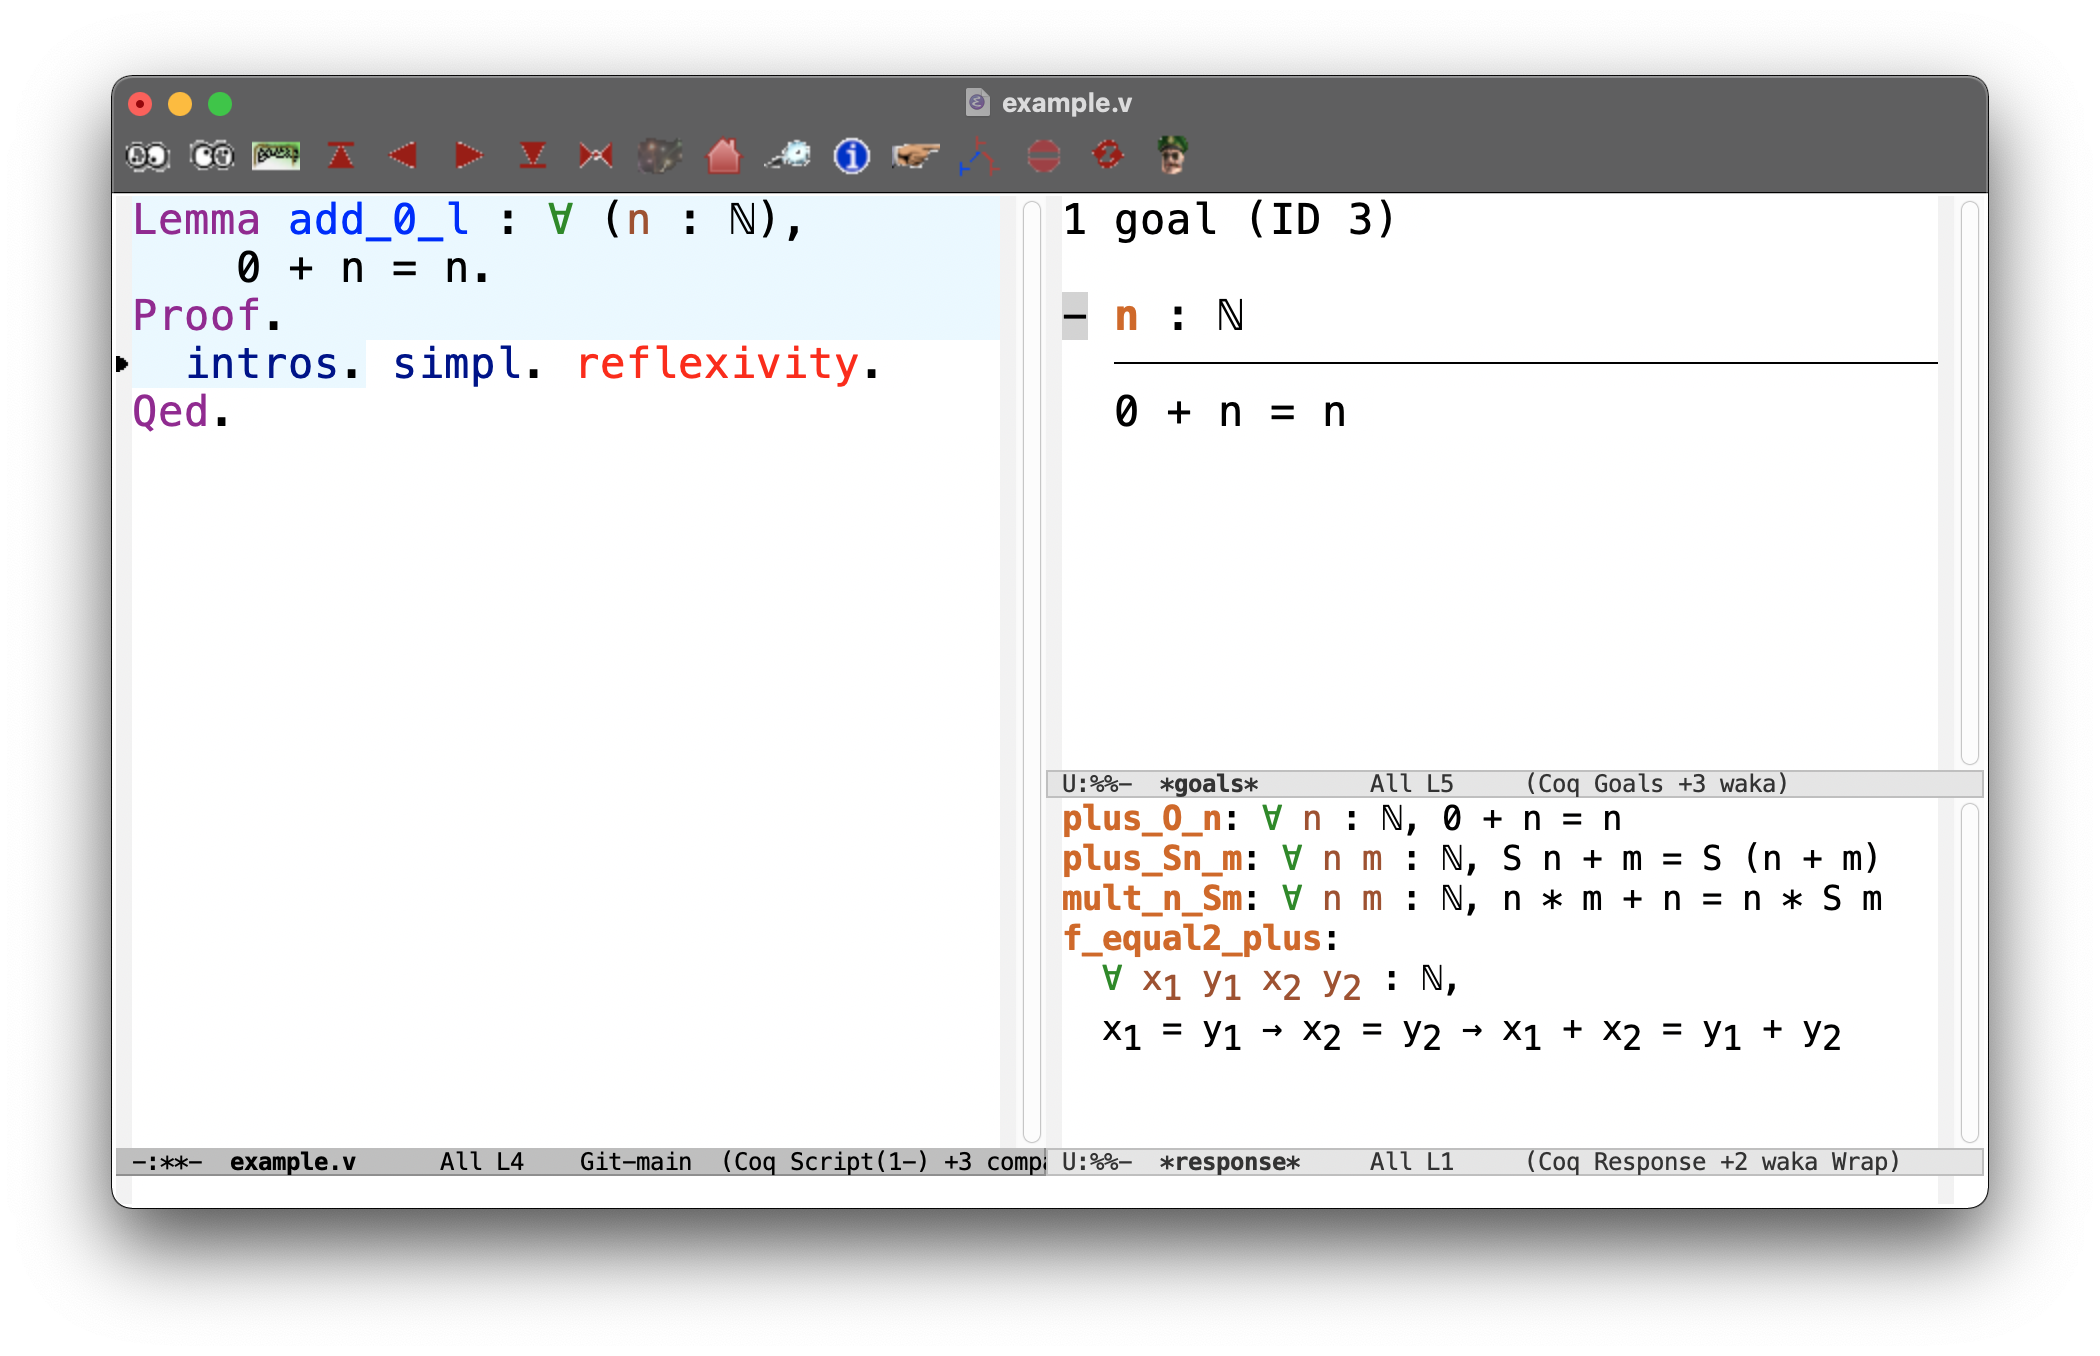
\includegraphics[width=.9\textwidth]{fig_ide}
\end{center}
\caption[Development view of the simple Rocq proof]
{A development view of the simple Rocq proof.
The Emacs editor is enhanced with the \href{https://proofgeneral.github.io/}{Proof General} interface
and the \href{https://github.com/cpitclaudel/company-coq}{Company-coq} plug-in.
The left view contains the proof code under development.
Focusing between \pr|Proof| and \pr|Qed| activates the {proof mode}.
While in proof mode, the {proof state} is visible in the top-right view.
The bottom-right view shows search results that appear after a database lookup for existing related lemmas.}
\label{fig:rocq-use}
\end{figure}

\paragraph*{Mathematical Components.}
The Mathematical Components library---colloquially mathcomp---extends the Rocq ecosystem with an extensive and coherent collection of formalized mathematical theories.
The library covers a wide spectrum of topics, including formal theory of general purpose data structures like lists;
prime numbers and finite graphs, and advanced topics in algebra.
The theories are organized into hierarchical levels where the design facilitates reuse.
The proof style is based on Rocq, but Mathematical Components uses a specialized language extension called SSReflect (small-scale reflection).
SSReflect significantly influences proof writing style and poses its own learning curve.
To demonstrate the difference,~\autoref{sm-tool-examples} shows examples in \enquote{standard} Rocq and SSReflect.
The Mathematical Components library has an essential role in the Rocq community because several landmark results of finite group theory are based on it.
For example, the mechanical proofs of the Four Colour theorem~\cite{gonthier2008} and the Odd Order theorem~\cite{gonthier2013} utilize the library extensively.

\paragraph*{Demonstrated applications.}
Conventional uses of Rocq include proving properties of programming languages, formalizing mathematics, and teaching.
\autoref{tab:rocq-results} contains representative examples across the first two categories.

\begin{table}
%! suppress = EscapeAmpersand
\begin{NiceTabularX}{\textwidth}{@{}l@{ }X@{}}
\toprule
\textbf{Formalization target} & \textbf{Authors} \\
\midrule
\href{https://users.dimi.uniud.it/~ivan.scagnetto/pi-calculus.html}{\(\pi\)-calculus in (Co)inductive-type theory} & \textcite{honsell2001} \\
\href{https://github.com/rocq-community/goedel}{Gödel-Rosser 1st incompleteness theorem} & \textcite{oconnor2005} \\
Modal model of impredicative semantics & \textcite{appel2007} \\
\href{https://github.com/rocq-community/fourcolor}{Four Color theorem}\smtabularnote{based on~\cite{robertson1997} and~\cite{appel1989}} & \textcite{gonthier2008} \\
\href{https://github.com/AbsInt/CompCert}{Verified Optimizing C Compiler, CompCert}\index{CompCert}\smtabularnote{A verifying compiler is one of the grand challenges for computing research posed in~\textcite{hoare2003}}\smtabularnote{CompCert received the ACM Software System Award in 2021.} & \textcite{leroy2009} \\
\href{https://gitlab.inria.fr/flocq/flocq}{Flocq: floating-point numbers} & \textcite{boldo2011} \\
\href{http://plv.csail.mit.edu/bedrock/}{Bedrock: low-level programming library} & \textcite{chlipala2011} \\
\href{https://github.com/davidnowak/bellantonicook}{Safe Recursion} -- \autoref{safe-rec} & \textcite{heraud2011} \\
\href{https://github.com/ProjectiveGeometry/ProjectiveGeometry}{Desargues's theorem in projective geometry} & \textcite{magaud2012} \\
\href{https://github.com/math-comp/odd-order}{Feit-Thompson's Odd Order theorem} & \textcite{gonthier2013} \\
\href{https://github.com/HoTT/Coq-HoTT}{Homotopy Type Theory} & \textcite{bauer2017} \\
\href{https://github.com/rocq-community/reglang}{Regular Language representations} & \textcite{doczkal2018} \\
\href{https://github.com/DeepSpec/InteractionTrees}{Recursive and impure programs} & \textcite{xia2019} \\
\href{https://github.com/uds-psl/coq-library-undecidability}{Undecidable Problems} & \textcite{forster2020b} \\
\bottomrule
\end{NiceTabularX}
\caption[The Rocq prover formalization results]{A small sample of results formalized with the Rocq prover.}
\label{tab:rocq-results}
\end{table}

\paragraph*{Additional resources.}
There are multiple literature sources for learning more about Rocq.
Coq'Art~\cite{bertot2004} is the first book dedicated to the proof assistant and its theory.
The \href{https://softwarefoundations.cis.upenn.edu/}{Software Foundations}~\cite{cpierce20221}
book series is a hands-on, active learning experience.
The books themselves are implemented in Rocq and updated regularly.
The Mathematical Components book~\cite{mahboubi2022} provides a guide to using the library and the SSReflect proof language.
Karate Coq of~\textcite{affeldt2023} is an additional resource about Mathematical Components.
There are multiple books about engineering Rocq proofs with dependent types and type systems~\cite{chlipala2022,chlipala2013,sergey2014,smolka2021}.
For a curated list of awesome Coq libraries, plugins, tools, and resources see the
\emph{Awesome Coq} list~\cite{awesome-coq}.
Finally, the Rocq prover has an active community, with discussion forums and a mailing list~\cite{rocq-community}.

\subsubsection{Dafny: The Verification Aware Programming Language}
\label{subsec:dafny}

Dafny is an open source verification-aware programming language, and a verifier for functional correctness~\cite{leino2010,dafnylang}.
Dafny was designed for reasoning, and it can automatically check programs against specifications during program development.
\autoref{fig:dfy-flow} shows a visual overview of the verification workflow.

\begin{figure}[ht]
\centering
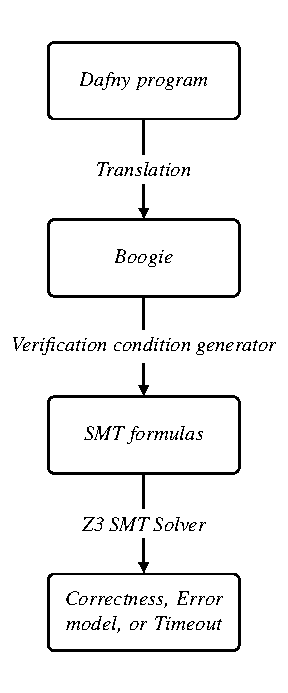
\includegraphics[width=\textwidth,keepaspectratio]{fig_dafny}
\caption[Overview of Dafny implementation and verification workflow]{
A (simplified) overview of Dafny implementation and verification workflow.
\enquote{A well-designed language and verifier, plus a great SMT solver, go a long way.} -- \textcite{leino2010b}.}
\label{fig:dfy-flow}
\end{figure}

\paragraph*{Technical overview.}
Dafny is a hybrid language, influenced by Java and C\#.
It has both functional and object-oriented features;
including: curly-bracket block-style, (mathematical) functions, and inductive and co-inductive data types.
The programming constructs include loops, \pr|if|-statements, arrays, classes and methods;
variables, types, generics, lambdas, inheritance, \etc~\cite{dafnydoc}
The real power of Dafny comes from the ability to annotate methods to specify their behavior.
For verification tasks, the idea is to define specifications and write proofs aside the implementation, in deductive verification-style.
The built-in verification constructs include pre- and postconditions;
loop invariants, termination metrics, lemmas, and ghost constructs\footnote{
A \emph{ghost} is any construct that is used for verification only; they are erased during compilation~\cite[p. 19]{leino2023}.}.
This language design enables writing functionally-correct verified programs fully in Dafny~\cite{leino2023}.
Dafny programs can be compiled to various target languages, like C\#, Java, and Go~\cite{dafnydoc}.

Dafny has an associated static program verifier.
The role of the verifier is to check a program's specification constructs\footnote{These are Eiffel-like contracts from~\cite{meyer1988}.}.
As visualized by the chart in~\autoref{fig:dafny-auto},
the built-in verifier in Dafny adds a high degree of automation, which resolves many low-level proof steps.
For example, if we wanted to prove the lemma of~\autoref{lst:rocq-basic} in Dafny, the verifier succeeds at discharging the proof obligations automatically -- see \pr|Add0Left| in~\autoref{fig:dafny-use}.

\begin{figure}[ht]
\centering
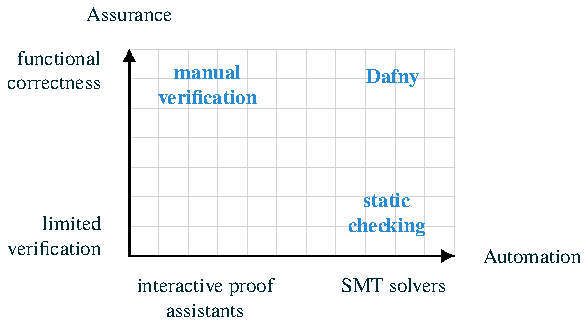
\includegraphics[width=.7\textwidth,keepaspectratio]{fig_chart}
\caption[Automation degree chart]{Automation degree -- a chart inspired by~\cite{leino2010b}.}
\label{fig:dafny-auto}
\end{figure}

\begin{figure}[p]
\begin{center}
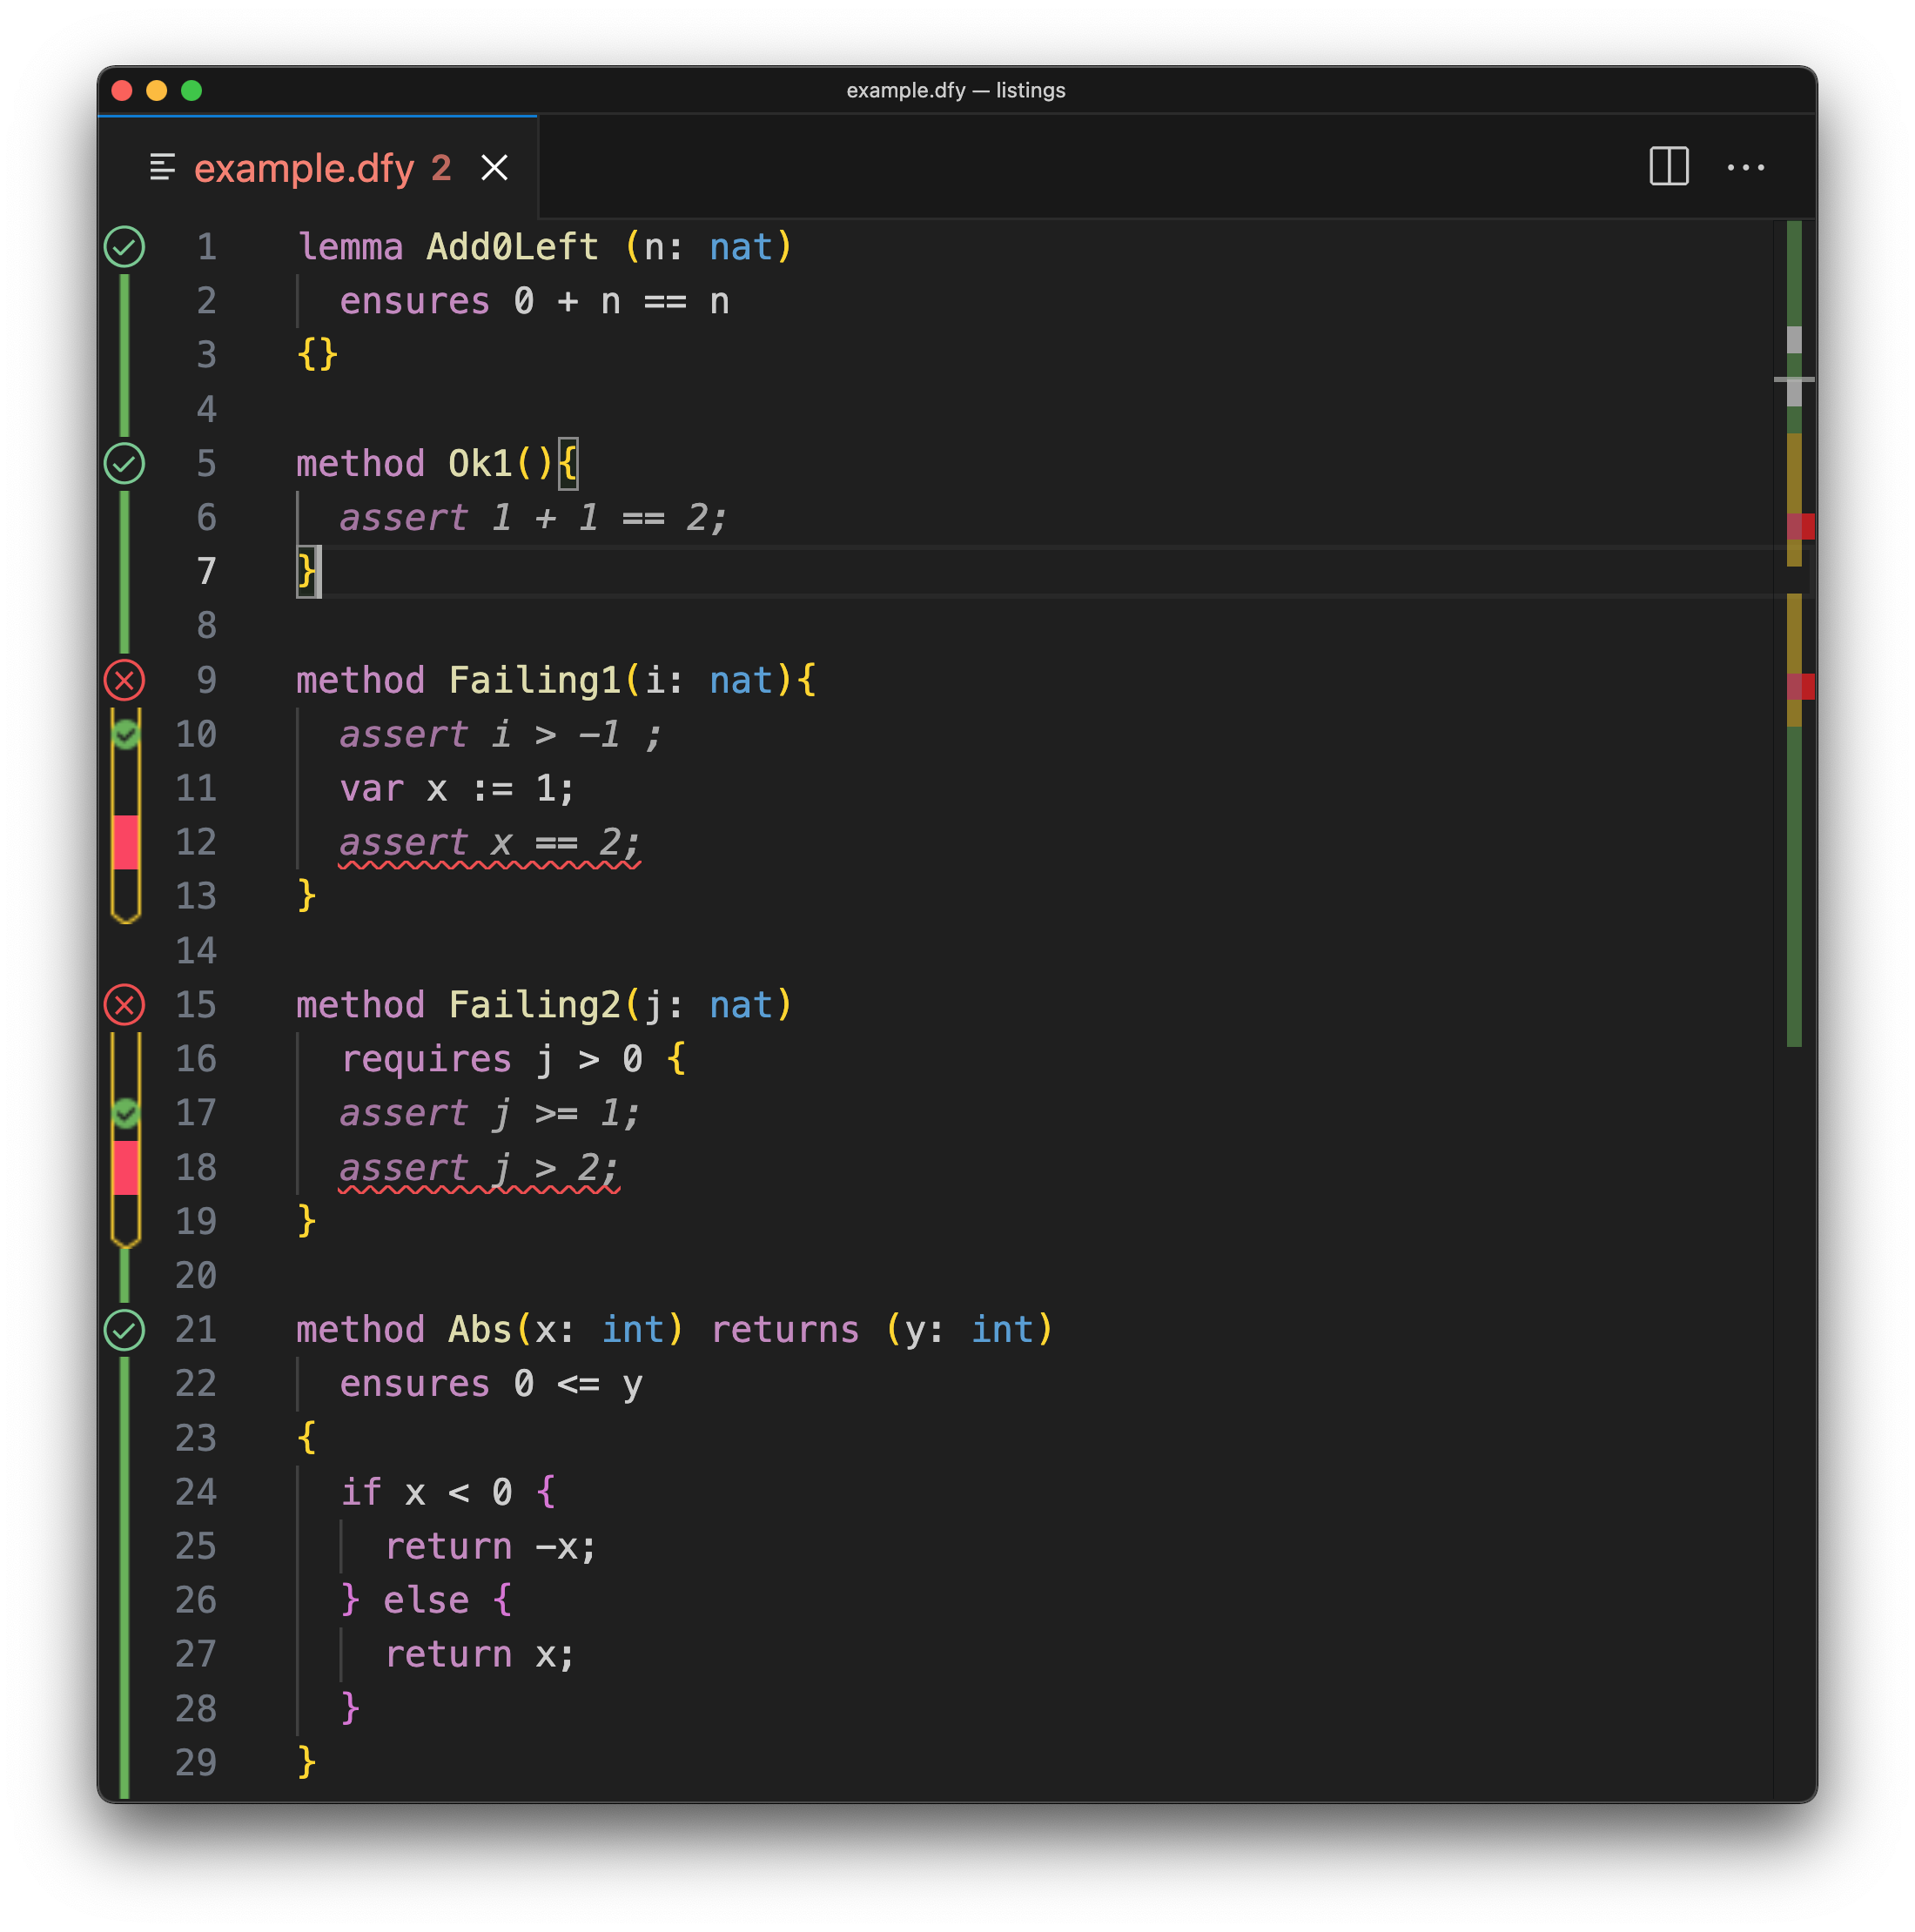
\includegraphics[width=\textwidth,keepaspectratio]{fig_vs1}
\end{center}
\caption[Dafny running in Visual Studio Code]{
The Dafny verifier checking Dafny code (running in Visual Studio Code).
A big green check{ }{ }\circledb[dafnyok]{\faCheck}{ }means the verifier succeeds at proving the corresponding program construct.
A big red cross{ }{ }\circledb[dafnyno]{\scalebox{1.25}{\faTimes}}{ }identifies program constructs that fail to verify completely, even if some inner declarations succeed.
A green filled check {\color{dafnyok}{\scalebox{.8}{\faCheckCircle}}} means the verifier succeeds at the proof obligation at the corresponding line.
The verification fails at declarations marked with a red block \langclr{dafnyred} and\;\;\uwave{squiggly underline}{}.
}\label{fig:dafny-use}
\end{figure}

A program accepted by the Dafny verifier is guaranteed to be totally correct, \ie it terminates and satisfies its specification.
During program development and when given a candidate specification, the verifier runs automatically on code edits, as shown in~\autoref{fig:dafny-use}.
The engineer receives immediate feedback on their verification efforts.
When Dafny verifier fails, the user must annotate the program with additional guidance---assertions, pre-conditions, lemmas, \etc---to assist the verifier, until the verification succeeds.
Logical contradictions, like the ones raised in~\autoref{fig:dafny-use}, will obviously never succeed.
The verifier helps to catch such errors early in the program development phase.

\paragraph*{Proof style.}
In Dafny, proofs are developed in \enquote{top-down} style.
This allows the developer to focus on the proof architecture before the detailed proof steps.
To this end, Dafny provides the constructs of \pr|assume| statements, \ie assertions without a proof;
and ghost methods, \ie lemmas that are not yet proven.
Obviously, the proof is not complete until these temporary constructs have been replaced with concrete proofs.
However, they are useful for facilitating the proof development.

\paragraph*{Boogie.}
{Boogie}~\cite{leino2008}\index{Boogie} is an intermediate verification language, used in the verification workflow of Dafny programs (\cf~\autoref{fig:dfy-flow}).
More generally, Boogie is an open source modeling language and a verification tool for sequential and concurrent programs, and distributed systems~\cite{boogie}.
It provides a layer on which to build program verifiers\footnote{
Several program verifies are built on Boogie, for example Dafny, Chalice, Spec\#, and Move~\cite{boogie}.}.
When viewed as a verification tool, Boogie takes as input a program written in the Boogie language.
Then, the tool infers invariants, generates verification conditions, and passes them to an SMT solver.
The default SMT solver is Z3~\cite{demoura2008}.

\paragraph*{Applications of Dafny.}
Dafny is a mature, industry-grade tool for program verification.
It has been used in research projects, industrial applications, verification projects, and in teaching formal methods.
Among the hallmark results, the AWS authorization engine---that handles 1 billion API calls per second~\cite{wagner2024}---is verified in Dafny~\cite{chakarov2025}.

\subsubsection{Tool Comparison by Light Examples}
\label{sm-tool-examples}

This section covers two verification tasks that are suitable for paper presentation while illustrating differences between the formal proof techniques.
To match the dissertation theme, the examples are about program proofs.
However, proving programs is only a subset of the general utility of these tools;
refer to \autoref{tab:rocq-results} for more cases.

\paragraph{Program Equivalence}

\autoref{lst:intro} in the introduction showed two programs with a claim that the programs are equivalent.
Equivalence means that, for all inputs, they compute the same result.
With manual inspection, one can become reasonably convinced that the claim is true.
However, such inspection provides only weak informal guarantees.
We can do better -- we now have the tools to prove formally the claim about equivalence.

\begin{center}
\begin{minipage}{\textwidth}
\captionsetup{type=lstlisting}
\rocqinputlisting[][firstline=175]{equiv.v}
\captionof{lstlisting}[A Rocq proof of program equivalence]{A Rocq proof of program equivalence (theorem only).
The full proof with the programming language syntax, semantics, and notations is about 200 LOC.}
\label{lst:eq-proof}
\end{minipage}
\end{center}

\subparagraph*{The Rocq proof explained.}
The Rocq theorem (L5--8) makes explicit that the equivalence holds when
\pr|X| and \pr|Y| are arithmetic expressions that evaluate to a \(\mathbb{N}\); \pr|Z| is a variable, and \pr|b| has value \(0\) or \(1\).
The precise programming language semantics are defined as part of the full proof.
The property of \emph{equivalence} is defined as a proposition (L1--3).
Informally, two programs (commands, \pr|c1| and \pr|c2|) are equivalent
iff they start execution in the same state (\pr|st|) and reach the same final state (\pr|st'|), for all states.
Although program termination is not guaranteed by this specification,
the state-based definition requires that equivalent programs must agree on divergence.
That is, if one program diverges, the other must diverge also.
The actual proof steps, in L9--23, show how to establish equivalence of the programs in~\autoref{lst:intro}.
At a high level, the proof proceeds as follows.
First, we split the bijection (\( \leftrightarrow \)) to inspect both directions of the equivalence.
Next, we substitute \pr|b| with concrete values, which creates additional subcases.
Some of these cases are contradictory and resolved easily by the \pr|discriminate| tactic (L13).
The proof concludes by applying algebra on the multiplication operations;
that is then sufficient to prove equivalence (L16, L22).
Without technical familiarity, the steps may not be easily readable from the tactics.
Yet, as for all mechanized proofs, it is possible for everyone to check the proof by compiling it.
Further, it is possible to inspect the proof steps in an editor or IDE\footnote{
Since the proof includes much symmetry and automation,
the proof needs some editing to reduce the automation before inspecting the intermediate steps.}.
Thus, a mechanized proof lifts the observer's need to understand the details of the proof to \enquote{just} understanding the stated theorem, and trusting the proof assistant with checking it.

\begin{center}
\begin{minipage}{\textwidth}
\captionsetup{type=lstlisting}
\dafnyinputlisting[][]{equiv.dfy}
\captionof{lstlisting}[Proof of program equivalence in Dafny]{
Program equivalence verified in Dafny (complete).
The listing includes a subtype definition of \pr|bit| that does not occur in the Rocq version.}
\label{lst:eq-dafny}
\end{minipage}
\end{center}

\subparagraph*{The Dafny verification explained.}
The Dafny version in~\autoref{lst:eq-dafny} contains the full details of the proof.
To make life a bit more interesting, it defines a subtype of \pr|bit|.
Alternatively, the restriction on the values of \pr|b| could be stated as a precondition.
Next, the listing shows a \pr|function| and a \pr|method|.
A \emph{method} in Dafny is a piece of imperative executable code, which can have all sorts of statements in its body.
The term \emph{function} is reserved for constructs that can be used directly in specifications.
Unlike a method, a function body must consist of exactly one expression, and it returns a value.
For the ways the two programs were originally written and for demonstration,
it makes sense to define the programs as a function and a method\footnote{
Specifying two methods is also possible, the proof will just look different.}.
Because \pr|Program2| is a function, it can be used in the specification condition of \pr|Program1|.
The \pr|ensures| clause says the value computed by \pr|Program1| is exactly equal to that
computed by \pr|Program2|, for all arguments.
The equivalence holds in both directions.
Because the equivalence is generally easy to show, the verifier succeed without additional lemmas,
which proves the equivalence claim.

\paragraph{Formally verified leftpad.}
Leftpad is a string manipulation function.
It pads a string, using a specified character, up to a specified length.
The padding character is applied to the left side of the string, as a prefix, hence the name.
\autoref{lst:leftpad} shows examples of leftpad behavior.

\begin{center}
\captionsetup{type=lstlisting}
\begin{minipage}{\textwidth}
\begin{minipage}{.45\textwidth}
\cmdinputlisting{leftpad.cmd}
\end{minipage}%
\hfill\(\Rightarrow\)\hfill%
\begin{minipage}{.45\textwidth}
\outinputlisting[][numbers=none]{leftpad.output}
\end{minipage}
\end{minipage}
\captionof{lstlisting}[Leftpad in action]{Leftpad in action.}
\label{lst:leftpad}
\end{center}

The \href{https://github.com/hwayne/lets-prove-leftpad}{\enquote{Let's Prove Leftpad}}~\cite{leftpad} is public challenge project initiated by Hillel Wayne.
The idea is to put different verification tools and proof techniques to test by using them to prove leftpad.
At the time of writing this (April 2025), the repository contains 29 variants of leftpad proofs.
The challenge is interesting, because a leftpad proof is small enough to be accessible without formal methods background, yet complex enough to differentiate the proof techniques.
The leftpad implementation is simple, but the formal specification is surprisingly tricky.
A formal proof requires showing that the following three specification conditions hold.

\begin{enumerate}
\item Given pad length \(n\) and a string \pr|str|, the output length is \(\max(n, \text{len}(\prm{str}))\).
\item The output prefix is padding characters and nothing but padding characters.
\item The suffix of the output is the original string \pr|str|.
\end{enumerate}

Listings~\autoref{lst:rocq-leftpad}--\ref{lst:leftdfy} show the complete implementations and proofs of leftpad in Rocq;
the SSReflect of the Mathematical Components library, and Dafny.
The proofs come from the \enquote{Let's Prove Leftpad} project repository~\cite{leftpad}.
They were originally crafted by Ezra Cooper (Rocq), Anton Trunov (SSReflect), and Hillel Wayne (Dafny).
The proofs are modified for paper presentation and to resolve language updates, with the Rocq proof modified heavily from its original form.
The padding character is represented as \pr|c|, the pad length is \pr|n|, and the input \enquote{string}\footnote{
    None of the proofs actually refer to \emph{string} type, though one uses a sequence of characters.} is \pr|s|.
Each version includes an implementation and a proof to show that the implementation satisfies the specification.

\begin{center}
\captionsetup{type=lstlisting}
\rocqinputlisting[breakable][]{leftpad.v}
\captionof{lstlisting}[Leftpad in Rocq]{Leftpad in Rocq.}
\label{lst:rocq-leftpad}
\end{center}

\subparagraph*{Leftpad in Rocq.}
The Rocq proof of leftpad is shown in~\autoref{lst:rocq-leftpad}.
The leftpad implementation (at L27--28) is intuitive --
it works by concatenating \(n - \text{length}(\prm{s})\) count of  symbols \pr|c| with \pr|s|.
Since the proof compiles successfully, we also know the leftpad implementation is guaranteed to terminate.
In the proof, the key idea is that it is possible to cut the concatenated string to a prefix and suffix, at index \(m\).
The specification is then proved \wrt the prefix and suffix, and the concatenated length.
Proving the theorem requires introducing the supporting definitions and lemmas of L6--25.

\subparagraph*{Leftpad in SSReflect.}
The Mathematical Components library does not contain definitions of string or character types,
which is why~\autoref{lst:mathcomp-leftpad} is generalized to a parametric type \pr|T|.
The leftpad implementation, at L8--9, is functionally the same as in~\autoref{lst:rocq-leftpad},
only expressed in the style of mathcomp.
The three lemmas that follow prove the specification.
The first lemma \pr|length_max_spec| matches the Rocq version in~\autoref{lst:rocq-leftpad},
but the prefix and suffix proofs are achieved differently.
The latter rely on a random access function \pr|nth| that returns the \(i\)-th element in a sequence
(numbered from 0), or the \pr|def| element, if the sequence contains fewer than \(i+1\) elements.
In the proofs, the imported libraries provide much assistance.
In SSReflect, it is common for simple proofs to require only rewrites, while \enquote{interesting proofs} appear visually longer.
The leftpad proof is simple since it requires only rewrites, and those rewrites are defined by the library.
The tactics naming convention is a design feature of the Mathematical Components library.
The naming eases locating proofs;
otherwise, one must search the proofs database.

\begin{center}
\captionsetup{type=lstlisting}
\begin{minipage}{\linewidth}
\mathcompinputlisting[][]{leftpad-ssrefl.v}
\captionof{lstlisting}[Leftpad in SSReflect proof language]{Leftpad in the SSReflect proof language of the Mathematical Components library.}
\label{lst:mathcomp-leftpad}
\end{minipage}
\end{center}

\begin{center}
\begin{minipage}{\linewidth}
\captionsetup{type=lstlisting}
\dafnyinputlisting[][]{leftpad.dfy}
\captionof{lstlisting}[Leftpad formally verified in Dafny]{Formally verified leftpad in Dafny.}
\label{lst:leftdfy}
\end{minipage}
\end{center}

\subparagraph*{Leftpad in Dafny.}
In Dafny, the specifications are \enquote{embedded} with the implementation.
To make the \autoref{lst:leftdfy} standalone, the \pr|Max| function is defined inline.
The three specification conditions correspond (in order) to the \pr|ensures| clauses.
The same conditions re-appear as loop invariants at L14--16.
The \pr|invariant| clauses are necessary to convince the verifier that the conditions are preserved over iteration of the loop.
Enhancing the \pr|while| loop is sufficient for the verifier to succeed at proving the implementation meets the specification.
There's one more proof obligation for loops, which is to show termination.
The \pr|decreases| clause proves termination, which established total correctness of the \pr|LeftPad| method.

\subparagraph*{Observable differences.}
Although the leftpad behavior is consistently the same,
the examples show different styles of implementation and varying approaches to proving that the implementation is \emph{totally correct}.
The Rocq prover is very flexible in supporting various kinds of proofs and enables fine-grained control over the specification.
The \enquote{built-in} specification style of Dafny -- with pre-and postconditions, invariants, and termination -- is natural and powerful for proving programs.
Much of the power comes from automatic decision procedures, but can be challenging to debug if the verification fails.
In general, it is important to understand the mechanics of the selected tool, since a tool choice greatly influences the proof style and built-in capabilities.

\subsubsection{The Moscow Problem}
\label{subsec:moscow}

The next problem is a more involved and interesting for formal techniques and logic.
The problem was presented to me by Natarajan Shankar under the name \enquote{the Moscow problem}.
Although it is too simple for research, it is also too fascinating to be left in obscurity.
Therefore, it appears here, in my dissertation.

\paragraph*{Problem Description.}
Assume there are three people, \(\mathsf{A}\), \(\mathsf{B}\), and \(\mathsf{C}\)\@.
Seven natural numbers in 1--7 are distributed randomly among the people.
\(\mathsf{A}\) gets 1 number, and \(\mathsf{B}\) and \(\mathsf{C}\) get 3 numbers each.
The numbers are distinct, \ie no two people hold the same number;
and the distribution is secret, \ie it is unknown who holds what numbers.
The challenge is to design a message exchange that meets the following requirements.

\begin{enumerate}
\item \(\mathsf{B}\) sends one message to \(\mathsf{C}\) and from that message, \(\mathsf{C}\) knows what numbers everyone holds.
      (And similarly in reverse: \(\mathsf{C}\) sends one message to \(\mathsf{B}\)\ldots).
\item \(\mathsf{A}\) observes the messages but \(\mathsf{A}\) \enquote{does not learning anything}.
      In other words, \(\mathsf{A}\) cannot determine who holds what numbers based on the observed messages.
\end{enumerate}

Messages are exchanged in plain text and \(\mathsf{A}\) is aware of the mechanics of the exchange protocol.
The Moscow problem is to design a technique that meets the requirements.
The following solution is what I have developed in response to the problem.

\paragraph*{Informal Solution.}
Starting with a claim: it is sufficient to achieve the desired system with a message exchange where the message value is a single digit in 1--7.

The exchange is symmetric.
Therefore, instead of referring to \(\mathsf{B}\) and \(\mathsf{C}\), we say \emph{sender} and \emph{receiver}.
The sender calculates the exchanged value (the single digit) using only the numbers they hold.
The receiver calculates---using the single digit and number they holds---the number \emph{held by \(\mathsf{A}\)}.
Finally, the receiver deduces the numbers held by the sender.
There are three important functions.
\begin{enumerate}
\item \emph{Send} function that calculates the exchanged digit.
\item \emph{Receive} function that calculates number held by \(\mathsf{A}\).
\item \emph{Recover} function that deduces values held by the sender.
\end{enumerate}

The functions are defined as follows.
The universe is \(U = \{ x \mid 1 \leq x \leq 7 \}\).
Letting \(X\) be a set of numbers in \(U\), the numbers \enquote{outside} \(X\) are defined by
the set complement \(\overline{X} = U - X\).
Letting \(y\) be a number in \(U\), we \emph{encode} a value by
\[\text{E}(X, y) =
\begin{cases}
7, & \text{if } \Sigma\,\overline{X} + y\pmod{7} = 0 \\
\Sigma\,\overline{X} + y\pmod{7}, & \text{otherwise}
\end{cases}\]
Letting the set of numbers held by the \emph{sender} (\resp \emph{receiver}) be \(X_s\) (\resp \(X_r\)),
we define the function \emph{send} as \(\text{S}(X_s) = \text{E}(X_s, 7)\).
The send function produces the exchanged message value \(m\) that is observable to everyone.
The function \emph{receive} is \(\text{R}(X_r,m) = \text{E}(X_r, m)\),
and it produces the number held by \(\mathsf{A}\), denoted as \(a\).
The receiver calculates numbers held by the sender using the \emph{recover} function \(\text{Rec}(X_r, a) = U - X_r - a\).

\paragraph{Formal proof.}
The interesting bit is showing that the solution meets the specification.
The solution is provable in the Rocq prover.
We define first the messaging functions as shown in~\autoref{lst:moscow-fun}.

\begin{center}
\begin{minipage}{\textwidth}
\captionsetup{type=lstlisting}
\mathcompinputlisting[][firstline=28,lastline=37]{moscow.v}
\captionof{lstlisting}[Moscow messaging functions]{Implementation of the messaging functions. The \pr|t| is a triple of natural numbers and
\pr|T3| converts an arbitrary-length sequence (back) to a triple.}
\label{lst:moscow-fun}
\end{minipage}
\end{center}

The message exchange requirements are defined by two lemmas.
First, \enquote{\(\mathsf{C}\) (\resp \(\mathsf{B}\)) learns everything from one message} is stated formally as shown in~\autoref{lst:lemma-1}.
The lemmas essentially says the receiver (\pr|R|) recovers (some permutation) of numbers that match exactly those held by the sender (\pr|S|).
The \pr|send S| is the value of the exchanged message.

\begin{center}
\begin{minipage}{\textwidth}
\captionsetup{type=lstlisting}
\mathcompinputlisting[][]{lemma1.v}
\captionof{lstlisting}[Receiver knows sender]{First requirement formally -- receiver learns the numbers held by sender.}
\label{lst:lemma-1}
\end{minipage}
\end{center}

An \emph{allocation} (type \pr|alloc|) represents a distribution of numbers in \(U\)
between \(\mathsf{A}\), \(\mathsf{B}\), and \(\mathsf{C}\).
The second criterion is that \enquote{\(\mathsf{A}\) does not learn anything}.
We formalize this in~\autoref{lst:lemma-2}.
The lemma says, for every allocation of numbers and after observing both message exchanges between \(\mathsf{B}\) and \(\mathsf{C}\),
\(\mathsf{A}\) has \emph{insufficient information}
to determine with certainty what numbers everyone is holding.
In other words, any observed exchanges can be explained by at least two different allocations,
because there exists an alternate (different) \pr|alloc2| that explains the observations of \(\mathsf{A}\).

\begin{center}
\begin{minipage}{\textwidth}
\captionsetup{type=lstlisting}
\mathcompinputlisting{lemma2.v}
\captionof{lstlisting}[Person A cannot recover the allocation]{
Second requirement formally -- \(\mathsf{A}\) does not learn anything.}
\label{lst:lemma-2}
\end{minipage}
\end{center}

A complete machine-checkable implementation and proof is available in the dissertation artifact (\cf~\aref{app:sec:artifacts}), in file in \pr|moscov.v|.
Checking the proof requires an installation for Rocq Prover (v8.20) and Mathematical Components (v2.3.0) on the host system.
To machine-check, we compile the proof by running the command \pr|coqc moscow.v| in a terminal.
The expectation is the proof should compile without errors in \textasciitilde{}20s.
It does not print any terminal output.

The proof compilation also runs an extraction routine.
The extraction generates a certified OCaml program, \pr|message.ml|, from the messaging functions implemented in SSReflect.
Within in the dissertation artifact (\cf~\autoref{tab:pub-artifacts}), another program \pr|exchange.ml| is a {driver} for running the certified program.
The driver uses the certified program to perform a message exchange when run as shown in~\autoref{lst:run-exchange}\footnote{%
The last step assumes a tool \href{https://github.com/ocaml/ocamlbuild}{\texttt{ocamlbuild}} installed on the host.
It can be installed with the \href{https://opam.ocaml.org}{Opam package manager} by \pr|opam install ocamlbuild|.}.

\begin{center}
\captionsetup{type=lstlisting}
\begin{minipage}{\textwidth}
\cmdinputlisting{exchange.cmd}
\outinputlisting[][firstline=2,lastline=3]{exchange.output}
\end{minipage}
\captionof{lstlisting}[Running a certified message exchange]{Running a certified message exchange.
In this scenario, \(\mathsf{A}\) holds the number 2, and everyone observes the messages \enquote{4} and \enquote{5}.
This information is not enough for \(\mathsf{A}\) to learn what numbers \(\mathsf{B}\) (\resp \(\mathsf{C}\)) is holding.
However, by the end of the exchange, \(\mathsf{B}\) and \(\mathsf{C}\) are fully informed.}
\label{lst:run-exchange}
\end{center}

The presented moscow problem solution could be adjusted to a universe of \([0, 6]\) with a small change.
However, solutions to other modifications---\eg larger set of numbers, different allocations, or more people---are unknown.

\subsubsection{Connecting Formal Methods and ICC}
\label{icc-formally}

There are several ways to relate complexity theory and formal methods.
The features that distinguish implicit complexity from the classic complexity in theory, are the same features that make it a suitable target for formal reasoning.
A particularly strong motivator is that the programming language-based approach yields more natural definitions and proofs of central results than the classical approach~\cite{kristiansen2017}.

Formalization of a theory requires significant time and effort.
However, based on to the continued and demonstrated relevance of ICC results (\cf~\autoref{tab:icc-results});
the frequent absence of \emph{formal} proofs among those results, and the maturity of formalization techniques, the criteria for formalizing complexity is well-satisfied.
In other words, the significance and potential are sufficient to justify the effort of seeking formal guarantees.

\paragraph*{Existing results in formally verified complexity.}
There exists a (small) collection of result formalizing classic complexity theory (\cf~\autoref{coqpl-related}).
For example, universal Turing Machines~\cite{forster2020}, the \(\mathcal{O}\)-notation~\cite{gueneau2018},
and the Cook-Levin theorem~\cite{gaher2021}%! suppress = CollapseCite
\footnote{The Cook-Levin theorem states that Boolean SAT is NP-Complete~\cite{cook1971, levin1973}.}
have already been formalized.

Among works of implicit computational complexity, the hallmark result of Bellantoni and Cook was formalized by~\textcite{heraud2011}.
The Rocq library Cecoa enables proving that a user-defined function is polytime computable.
It is based on quasi-interpretations of~\textcite{marion2000} and extends the Bellantoni and Cook-formalization.
The Cecoa library is in-between complexity theory and analysis.
However, it is not an automatic program analyzer, since user-effort is needed to establish the complexity result.

To the best of our knowledge, no formalized automatic resource analyzer exists.
The closest to the goal are the analyzers C4B and Pastis (\cf~\autoref{resource-analysis-tools}),
that produce \emph{proof certificates} for the bounds they compute.
The AARA-based analysis technique is founded on inference rules, then which enables the derivation trees to be translated to machine-checkable proofs.
The certificates are produced via a support library that complements the core analysis.
However, the analysis {technique} is not proven correct.

\paragraph*{From implicit complexity towards formal methods.}
There is much room to improve the state-of-the-art in formal reasoning about complexity -- both in terms of theory and analysis.
Implicit computational complexity presents a potential avenue toward advancement.

Motivated by the various demonstrated applications, the flow calculus of mwp-bounds is an appealing target for formalization.
An important step is proving formally the mwp-calculus soundness theorem (\autoref{mwp-soundness}).
Such pursuit benefits from the facts that
(i) the paper proofs are available in~\cite{jones2009}, and
(ii) our confidence in the theory being correct is high (\ie if a problem existed, it likely would have surfaced in the prior projects).
However, converting the mwp-calculus to a formal proof---and in Rocq this means converting from set theory to type theory---poses various challenges.
Further, such proof would not extend to enhanced \textsc{mwp}$^\infty$-calculus variant of the calculus that is used in program analysis.
Yet, starting with the core mwp-calculus and paper proofs is a solid strategy toward formalizing complexity.
The result would extend broadly to all programs that share the same imperative core.
This project idea is discussed in~\autoref{sec:mwp-calc-formal}.

It is important to note the utility of implicit computational complexity is not limited to formalizing complexity results.
Another perspective is to use ICC systems in assisting formal methods tools in program verification efforts.
This is the motivating idea in the manuscript of~\autoref{sec:postcond}.
The central idea is that inferred mwp-bounds can be used as postconditions in Dafny-style deductive verification.

%The third goal is to strengthen the hypothesis that implicit computational complexity is naturally suited to formal reasoning.
%Classic complexity theory is predicated on machine models that are difficult to represent formally~\footnote{
%For example, a formal model of TMs in~\textcite{forster2020} took five years to complete.}.
%In contrast, the programming languages-based approach of implicit computational complexity makes formal reasoning more accessible.
%The findings of this dissertation are sufficient to motivate and justify the effort for undertaking rigorous formalization projects.

%----------------------------------------------------------------------------------------
%	2. PUBLISHED MANUSCRIPTS
%----------------------------------------------------------------------------------------
\chapter{Published Manuscripts}\label{ch:published-manuscripts}
% The candidate must be first author on all manuscripts bundled into the dissertation.

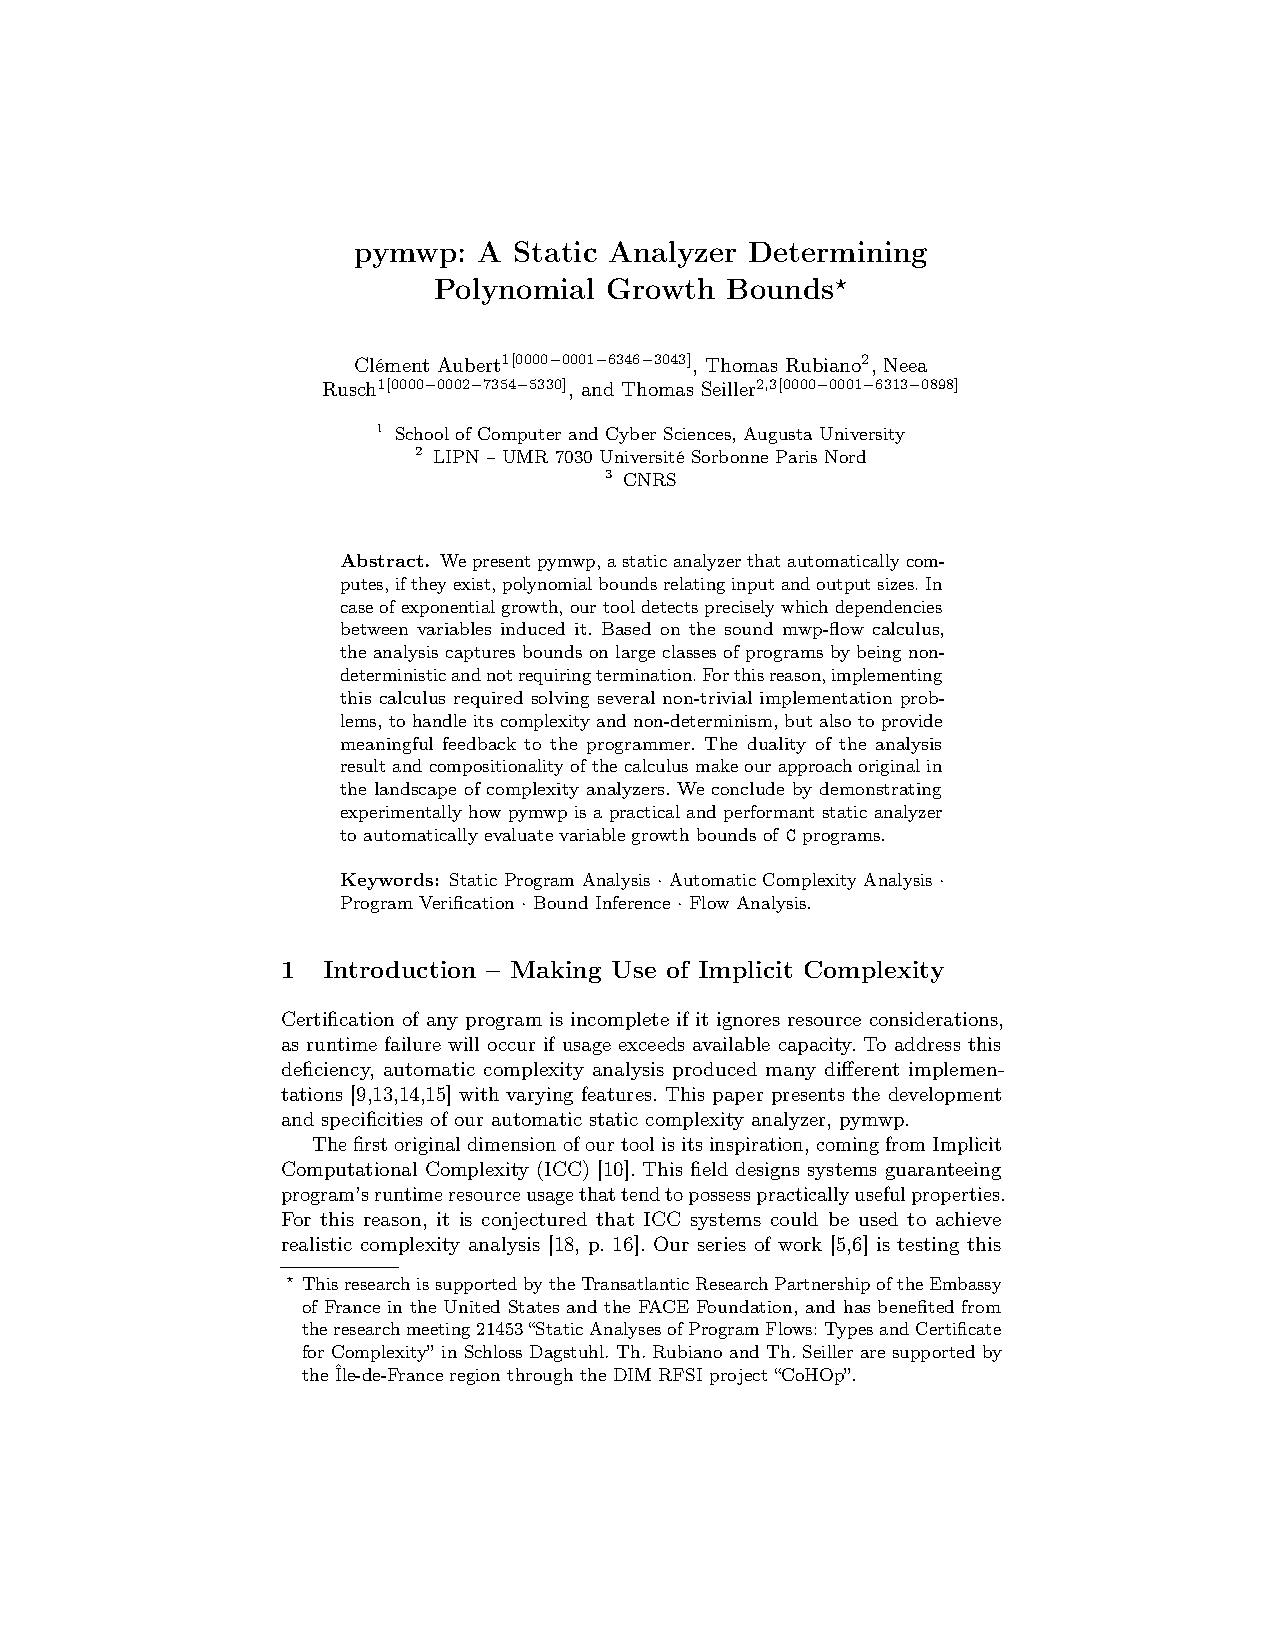
\includepdf[pages={1-},pagecommand={\thispagestyle{empty}\stepcounter{insertpages}
\ifnum\value{insertpages}=1\addcontentsline{toc}{subsection}{
pymwp: A Static Analyzer Determining Polynomial Growth Bounds}\fi
}]{papers/atva/main.pdf}\setcounter{insertpages}{0}

%----------------------------------------------------------------------------------------
%	3. UNPUBLISHED RESEARCH
%----------------------------------------------------------------------------------------
\chapter{Unpublished Research}\label{ch:unpublished-research}
% This can include manuscripts, in the journal format, that have been submitted for
% publication that are under review at the time of dissertation submission. Manuscripts
% that have been rejected or that have not been submitted (in preparation) cannot be
% included in the journal format (i.e. must conform to the traditional dissertation
% format). For manuscripts that have been submitted and are under review, the first
% authorship of the candidate must be maintained when the manuscript is published.

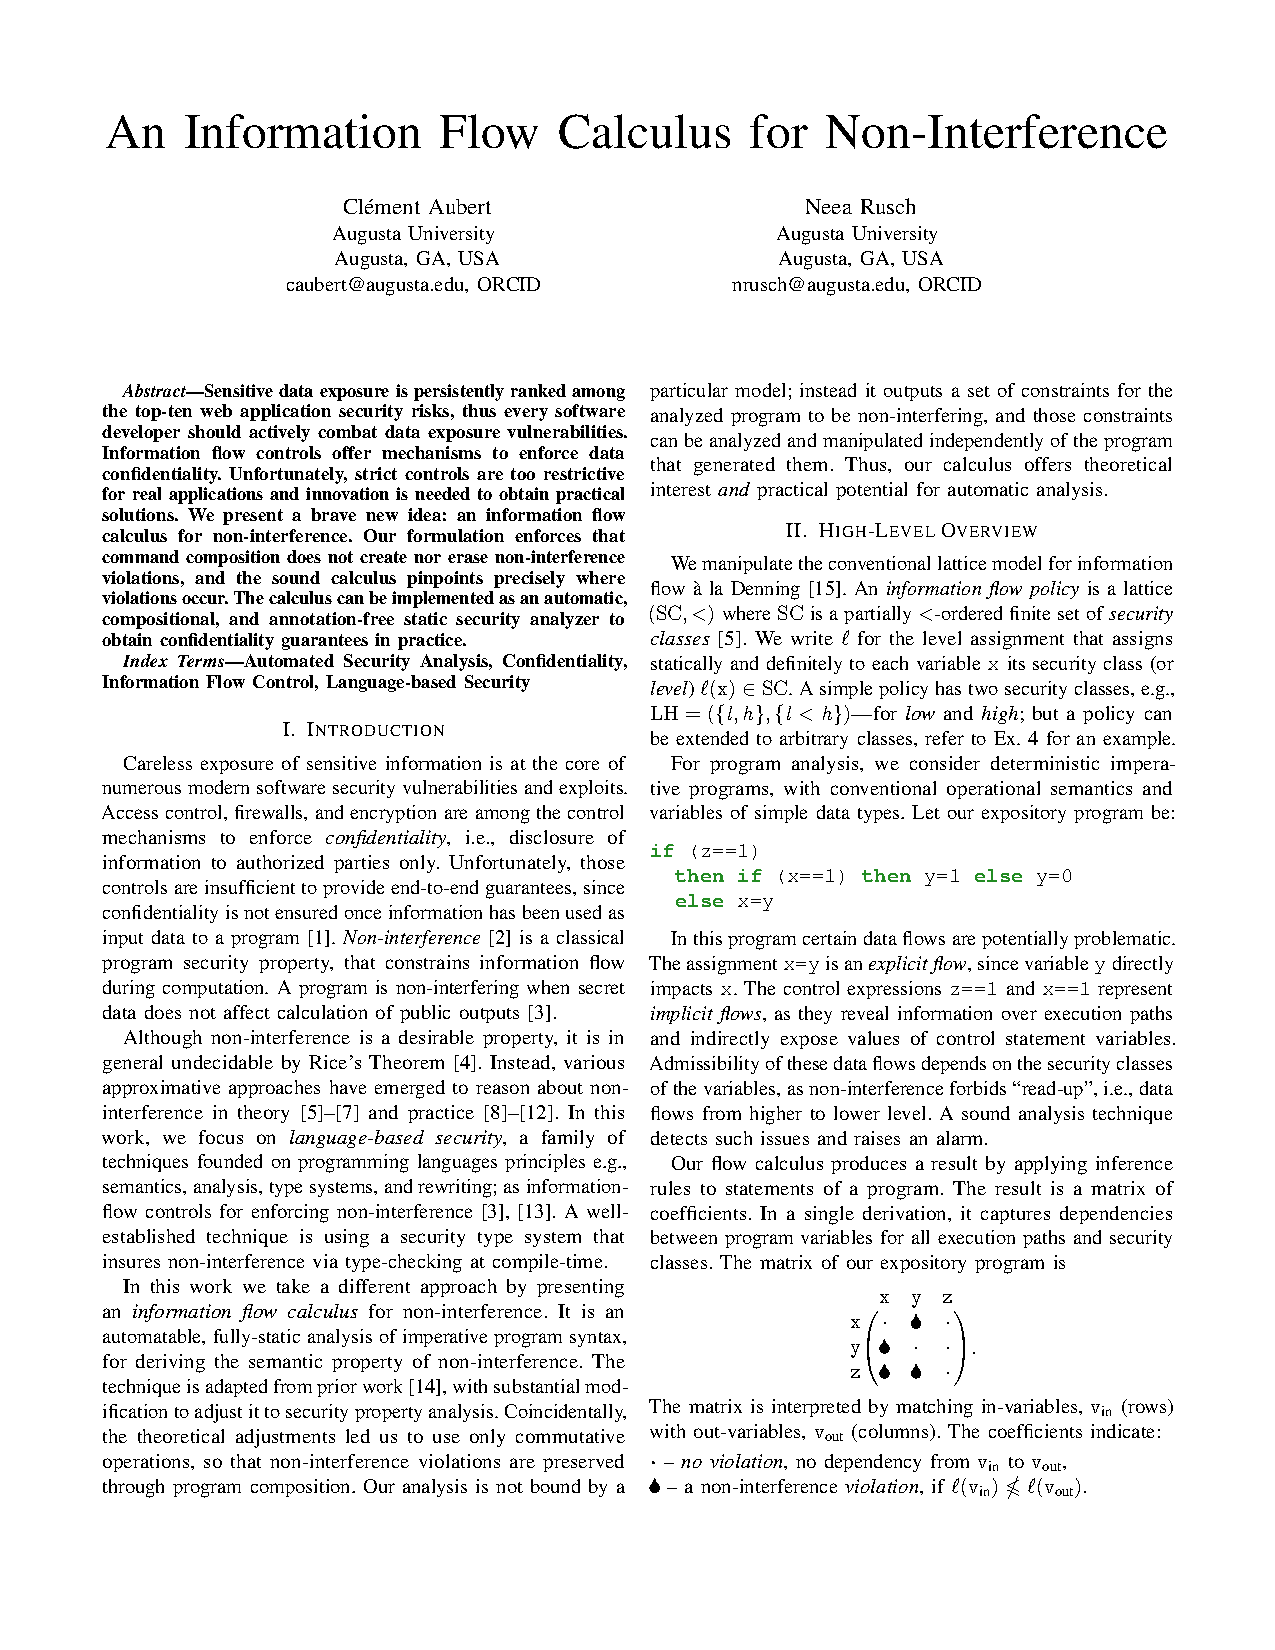
\includepdf[pages={1-},pagecommand={\thispagestyle{empty}\stepcounter{insertpages}
\ifnum\value{insertpages}=1\addcontentsline{toc}{section}{
An Information Flow Calculus for Non-Interference}\fi
}]{papers/plas/main.pdf}\setcounter{insertpages}{0}

\subsection{Motivation}\label{coqpl-motivation}

The ability to statically infer resource bounds of programs offers numerous benefits, \eg to insure safe memory usage.
Even more preferable if those guarantees are established with the rigor of formal verification,
because that increases confidence in the obtained analysis result and enables integration of complexity
analyses into larger formal developments.

Unfortunately, computational complexity is notoriously difficult to represent formally for several reasons.
In general, deriving a complexity bound for an arbitrary program is an undecidable problem.
In the area of complexity theory, \textcquote[p.~114]{forster2020}{%
formalisations of even basic complexity-theoretic results are not available}, hindering certification attempts.

For practical complexity analyses, many existing techniques present methodological challenges if they require
\eg program termination or inlining functions~\cite{carbonneaux2015}.
Therefore, a realistic pathway toward formal certification of a program's resource usage is narrow.
A few encouraging early results exist, and we discuss some of those in \autoref{coqpl-related}.
In this proposal we will sketch how a different approach, founded on Implicit Computational Complexity,
could sidestep some of the usual difficulties in implementing and verifying complexity analyses in Coq\index{Coq}.

The field of Implicit Computational Complexity (ICC)~\cite{dallago2011} drives better understanding of complexity classes, but it also guides the development of resources-aware languages and static source code analyzers.
The core idea is to bound resources \emph{while the program is being written (or type checked)} instead of measuring its resource usage afterwards on an abstract model of computation.
This can be done through \eg bounded recursion or using typing mechanisms.
The goal is to find a syntactical restriction or a type system such that a program can be written or typed only if it belongs to a particular complexity class.
ICC-based systems are often compositional, and they offer more natural tools to write programs than theoretical models of computation used in complexity theory.
We speculate these combined properties could make ICC-approaches a conceivable pathway toward certified complexity and sketch a more detailed plan below.

\subsection{Preliminary Action Plan}\label{coqpl-preliminary-action-plan}

We plan to formalize in Coq an ICC-based complexity analysis technique, the \emph{mwp-flow analysis}~\cite{jones2009}\footnote{%
Where mwp stands for \emph{m}aximum, \emph{w}eak polynomial and \emph{p}olynomial, representing increasing growth rates of variables values.}.
We chose this method because its internal mechanics has been recently studied~\cite{aubert20222}, and by our assessment, it seems suitable for formalization in Coq\index{Coq}.
As for Coq, it seems like the ideal target language because of its existing libraries and preliminary work--some of which are discussed in \autoref{coqpl-related}--, most notably related to compilers~\cite{leroy2009}.

\subsubsection{Overview of \emph{mwp}-Flow Analysis}\label{coqpl-overview-of-mwp-flow-analysis}

The \emph{mwp}-flow analysis certifies polynomial bounds on the size of the values manipulated by an imperative program.
While it does not ensure (or require) program termination, it provides a certificate guaranteeing that the program uses throughout its execution at most a polynomial amount of space, and as a consequence that if it terminates, it will do so in polynomial time in the size of its inputs.

The analysis computes, for each program variable, a vector tracking how it depends on other variables.
The vector values are determined by applying the nondeterminitic rules of the sound \emph{mwp}-calculus to the commands of the program.
Those vectors are collected in a matrix\index{matrix!mwp}.
A program is assigned a matrix\index{matrix!mwp} only if all the values in it are bounded by a polynomial in the inputs sizes.
This technique is compositional, abstracts away \eg iteration bounds, and operates on a memory-less imperative language, reminiscent of the \texttt{Imp} language from Software Foundations~\cite{cpierce20221}\index{Software Foundations}.

\subsubsection{The Coq Formalization}\label{coqpl-the-coq-formalization}

Our goal is to certify the analysis as presented in {the original paper}~\cite{jones2009}.
Note that this does not mean that the bound is certified, but that \emph{the mechanism to compute those bounds} is certified.
Of course, this implies the correctness of the bounds as a by-product but constitutes a major difference \wrt the results discussed in \autoref{coqpl-related}.
Preliminary explorations have led us to establish the following milestones.

\begin{description}
\item[The mathematical foundations]
Our first goal is to define the mathematical structure required to carry out the rest of the construction.
This requires defining vectors, matrices and their operations, semi-rings, and honest polynomials\index{honest polynomial}\footnote{%
Which are \textcquote[p.~5]{jones2009}{polynomial build up from constants in \(\mathbb{N}\) and variables by applying the operations \(+\) (addition) and \(\times\) (multiplication).}} that are needed to represent the \emph{mwp}-bounds\index{mwp-bound}.
The Mathematical Components library~\cite{mahboubi2022,mathcomp}\index{Mathematical Components} will lay the foundations for the linear algebra representations, but likely requires extensions to accommodate our specific analysis.

\item[Implementing the language]
The analyzed language is a simple imperative language that manipulates natural numbers, held in a fixed number of program variables.
Its syntax includes variables, expressions (operations \(+\) and \(\times\)), Boolean expressions, and commands
(\eg  assignment, loop and decision statements, command sequences, and skip), with their usual semantics.
We expect implementing it and its small-steps semantics\index{small-steps semantics} in Coq\index{Coq} to be relatively simple, following the examples from Software Foundations~\cite{cpierce20221,cpierce20222}\index{Software Foundations}.

\item[Implementing the typing system]
Even if it can be computationally expensive to run an automatic inference~\cite{aubert2023b}, the typing system \emph{in itself} is relatively simple.
It contains only 10 rules, essentially one for each type of command, and except for the initial assignment of vectors to variables, is fully deterministic.
We conjecture that standard methods~\cite{chlipala2022, chlipala2010} to implement simple type systems will be enough, but will require some care to scale to the matrix-as-type paradigm of this analysis.

\item[Certifying the analysis]
This will be the most demanding part of our plan.
The original paper contains all the required handwritten proofs, but the authors caution that
\enquote{\textins{t}hese proofs are long, technical and occasionally highly nontrivial}~\cite[p.~2]{jones2009}.
The main result of the paper is the soundness proof of the analysis~\cite[Theorem 5.3]{jones2009},
\ie the proof of the existence of a matrix\index{matrix!mwp} typing the program implies the existence of an honest polynomial\index{honest polynomial} bounding the variables' growth rates.
The main result follows from 15 pages of proofs presented in section 7 of the paper.
This section revolves around proving the soundness properties of the calculus, and we expect the most substantial effort to be spent on formalizing these proofs.
Some of them are quite intricate but with a satisfactory level of detail.
The cases concerning soundness of loops are the most difficult on paper, but their inductive nature \emph{should} (we hope!) be processed by Coq\index{Coq} rather easily.
\end{description}

We leave for future work the possibility of creating a formally verified, automatic static analyzer founded on the proof of correctness of this method: as we discussed in other works~\cite{aubert2023b,aubert20222}, care is required to implement a typing strategy that does not rapidly become intractable.

\subsection{Related Work}\label{coqpl-related}

A few prior results exist that combine formalization of complexity and Coq\index{Coq}.
They range from practical analyses to proofs in computational complexity theory.

For practical application, Coq has been used to verify stack bounds for assembly code~\cite{carbonneaux2014} and to obtain WCET loop-bound estimation~\cite{blazy2013}.
{Carbonneaux et al.}~\cite{carbonneaux2017} presented an automatic static analyzer for imperative programs, and although the analyzer itself is not verified, it generates bounds with machine-checkable certificates, to guarantee that the computed bound holds.
For functional paradigm, McCarthy et al.~\cite{mccarthy2018} developed a Coq\index{Coq} library, with a monad that counts abstract steps, which enabled running time analysis of programs written using the monad.
An ICC-based characterization was introduced by Férée et al.~\cite{feree2018}, in the form of a Coq\index{Coq} library, that allows for readily proving that a function is computable in polynomial time.

Coq\index{Coq} has also been used to formalize some of the foundations of modern complexity theory.
{Ciaffaglione}~\cite{ciaffaglione2016} proved the undecidability of the halting problem.
{Guéneau et al.}~\cite{gueneau2018} formalize the \(\mathcal{O}\)\symbo{bigo} notation.
{Forster et al.}~\cite{forster2020} implemented a multi-tape to single-tape compiler, and introduced the first formalized universal Turing Machine verified \wrt time and space complexity, for any model of computation, in any proof assistant.
More recently, Gäher and Kunze formalized the Cook-Levin theorem in Coq~\cite{gaher2021}.
Despite these advances, formalization of complexity is in early stages and basic complexity-theoretic results \eg time and space hierarchy theorems, remain unavailable.

Our proposed project differs from these earlier results primarily in its intent.
We plan to formalize the complexity analysis mechanism itself---not its computed result, as was done previously.
In their work with the Turing Machines, Forster et al.~\cite{forster2020} were explicit in emphasizing the challenge they experienced in formalizing complexity.
We hypothesize that our ICC-based approach, with \eg its built-in abstractions, will help reduce this challenge.
It is our hope that CoqPL will welcome our proposal for a certified complexity analysis in Coq\index{Coq}, and will be keen on indicating any library, tool or resource that could help.


%----------------------------------------------------------------------------------------
%	4. DISCUSSION
%----------------------------------------------------------------------------------------
\chapter{Discussion}\label{ch:discussion}
A comprehensive discussion that integrates the findings of all research presented
in the dissertation and that identifies how the goals or specific aims of the project
were attained, and how the research has answered the hypotheses put forth in the
dissertation.


%----------------------------------------------------------------------------------------
%	5. SUMMARY
%----------------------------------------------------------------------------------------
\chapter{Summary}\label{ch:summary}
A series of concise remarks summarizing experimental findings and conclusions


%----------------------------------------------------------------------------------------
%	6. REFERENCES
%----------------------------------------------------------------------------------------
\chapter{References}\label{ch:references}
% All literature cited in the dissertation will be included here. Style should conform
% to selected style manual. References included in manuscripts must be renumbered and
% reformatted (if needed) and included in this section. Literature Cited sections within
% the manuscripts should be omitted.
\printbibliography[heading=none,sorting=none]

%----------------------------------------------------------------------------------------
%	7. APPENDICES
%----------------------------------------------------------------------------------------
\chapter{Appendices}\label{ch:appendices}

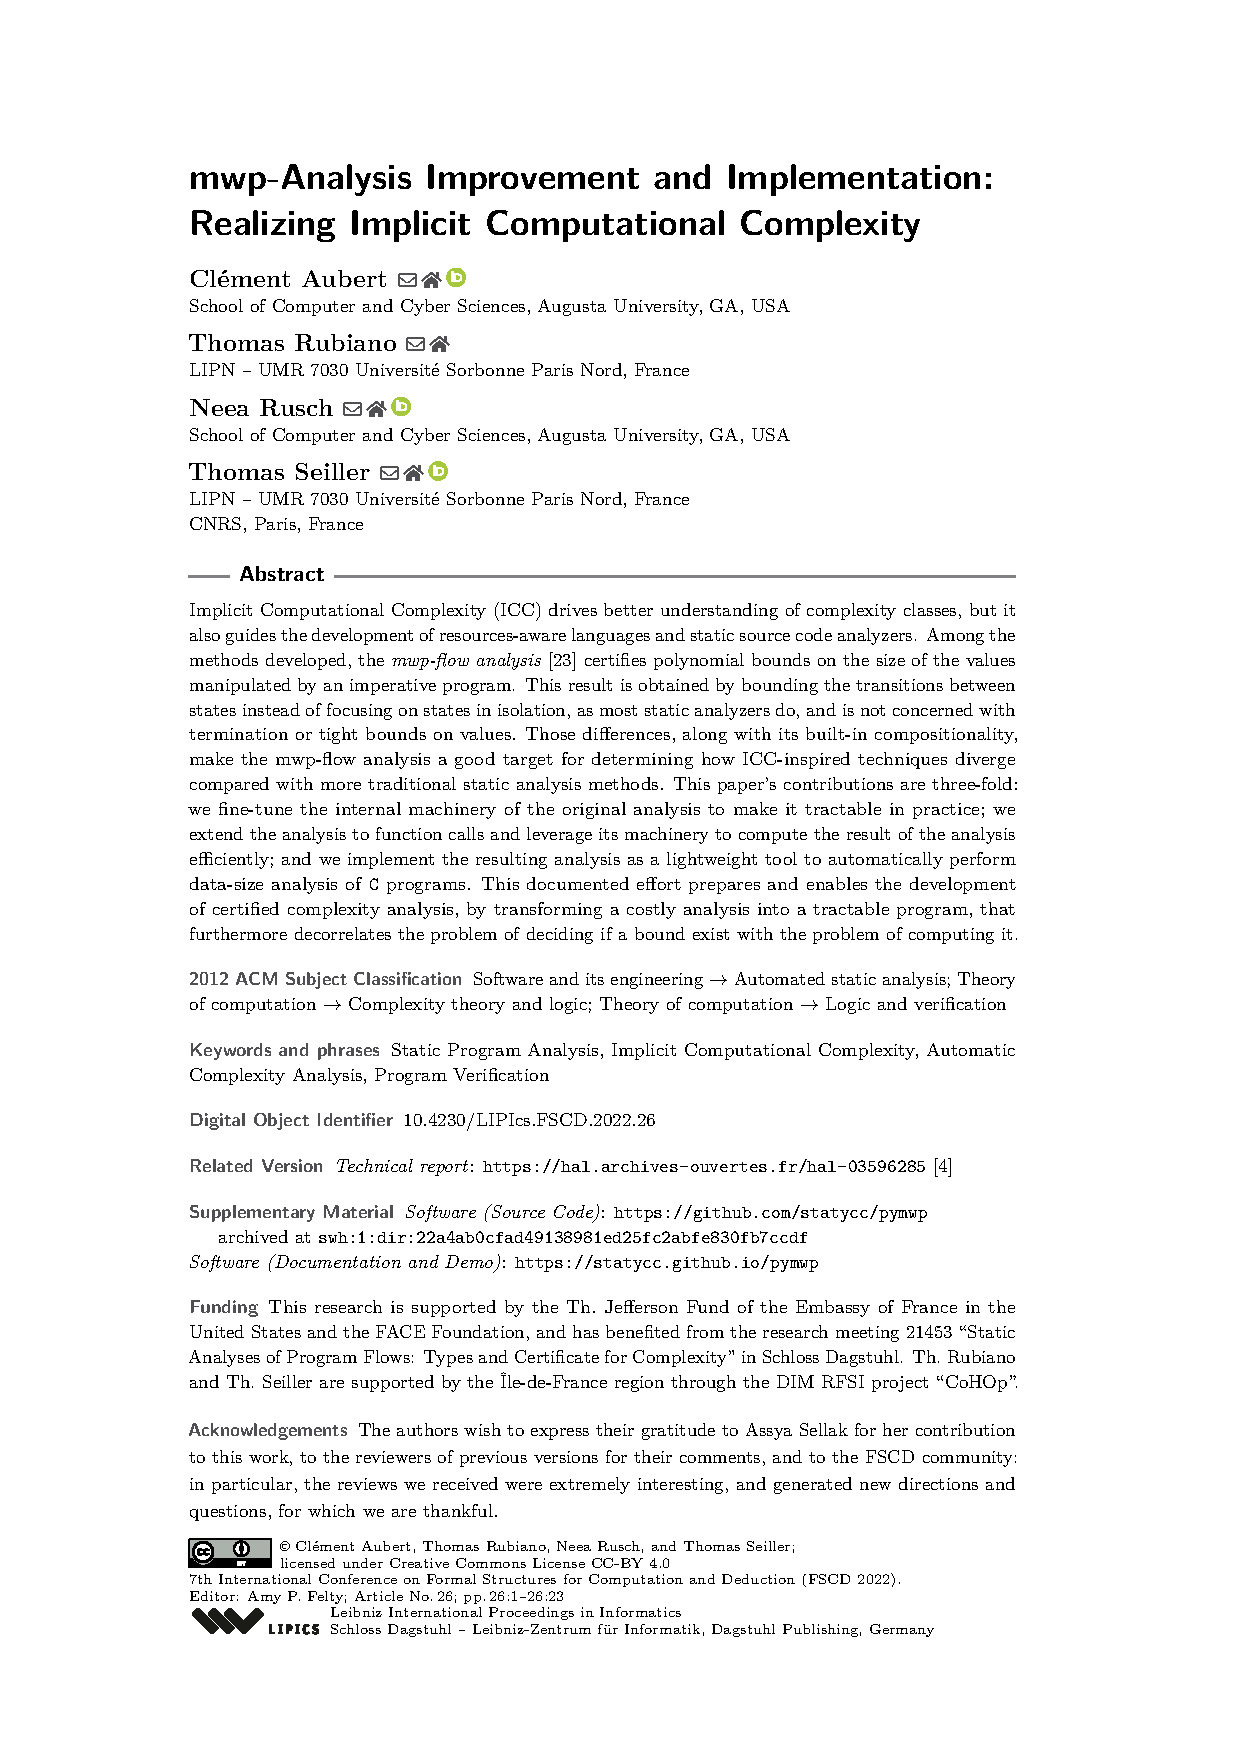
\includepdf[pages={1-},pagecommand={\thispagestyle{empty}\stepcounter{insertpages}
\ifnum\value{insertpages}=1\addcontentsline{toc}{section}{
mwp-Analysis Improvement and Implementation: Realizing Implicit Computational Complexity}\fi
}]{res/pubs_fscd.2022.pdf}\setcounter{insertpages}{0}

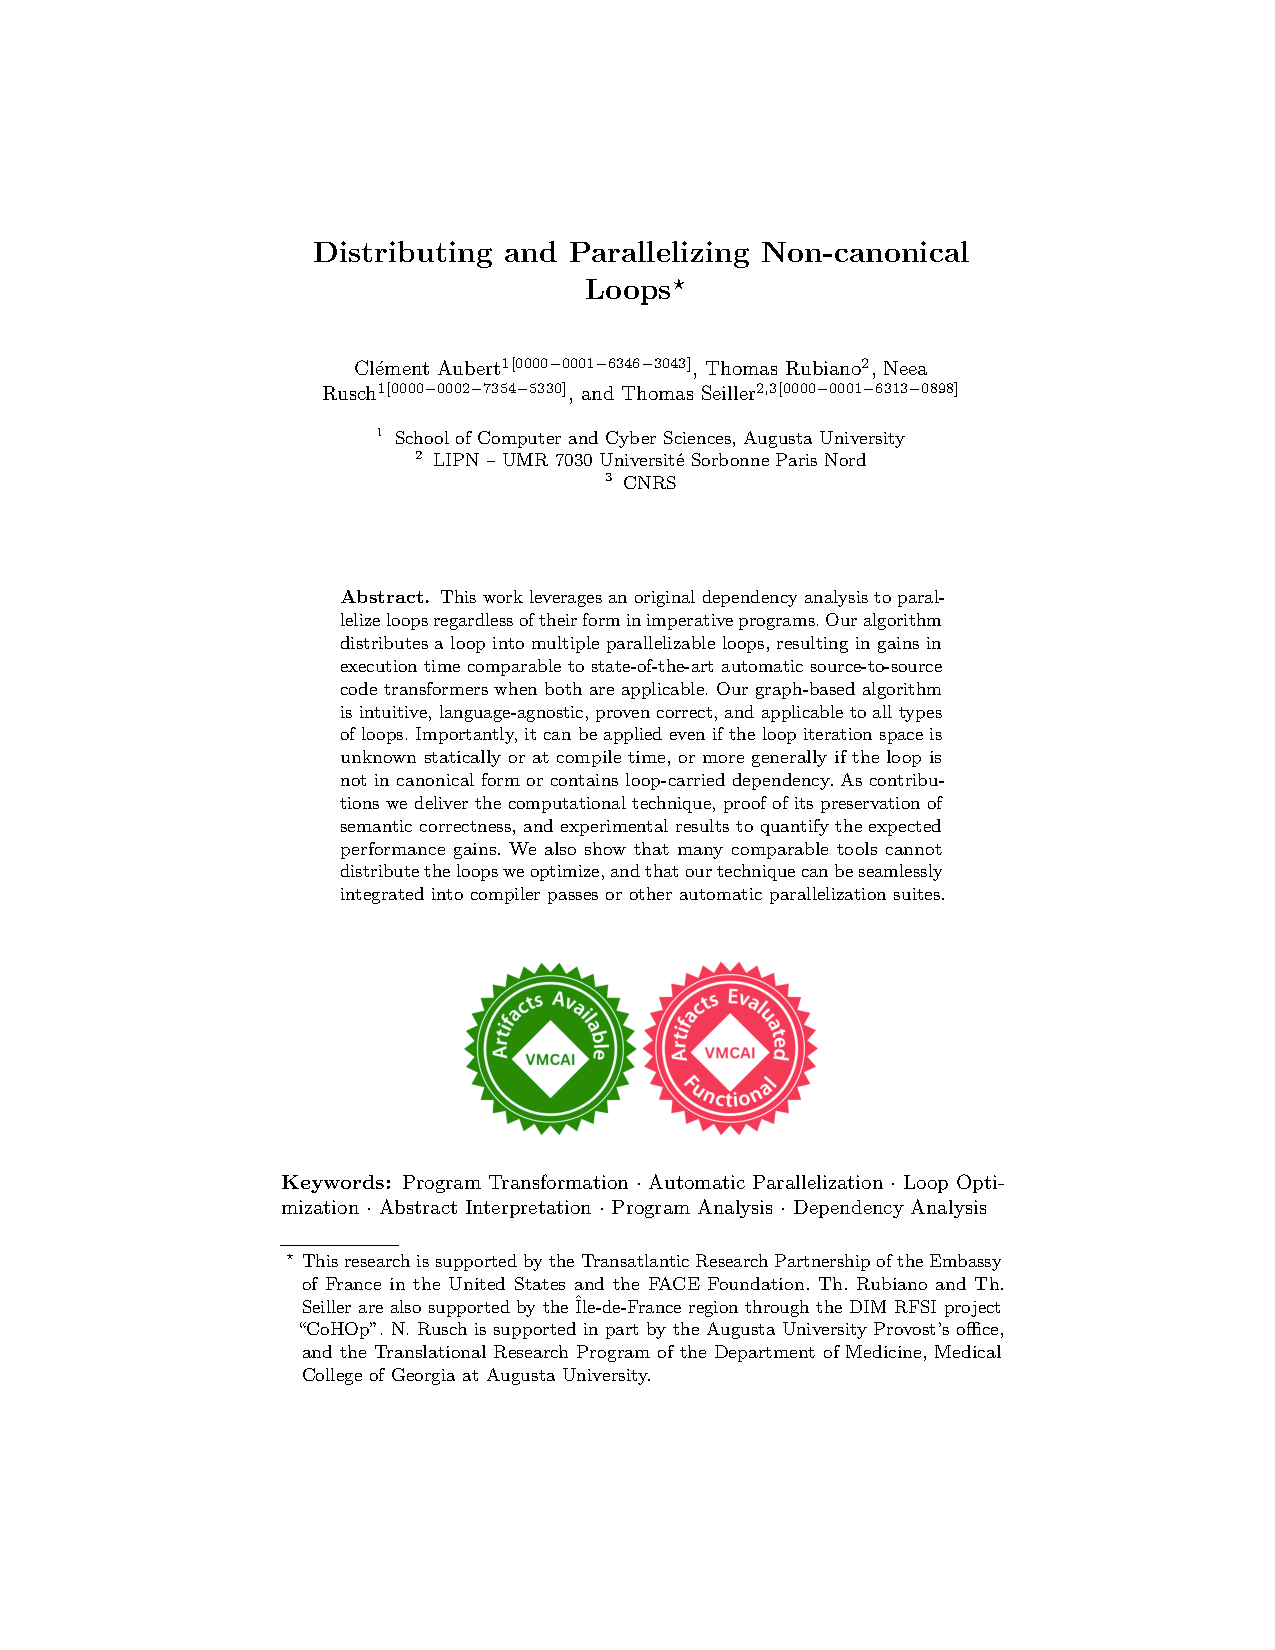
\includepdf[pages={1-},pagecommand={\thispagestyle{empty}\stepcounter{insertpages}
\ifnum\value{insertpages}=1\addcontentsline{toc}{section}{
Distributing and Parallelizing Non-canonical Loops}\fi
}]{res/pubs_vmcai.2023.pdf}\setcounter{insertpages}{0}

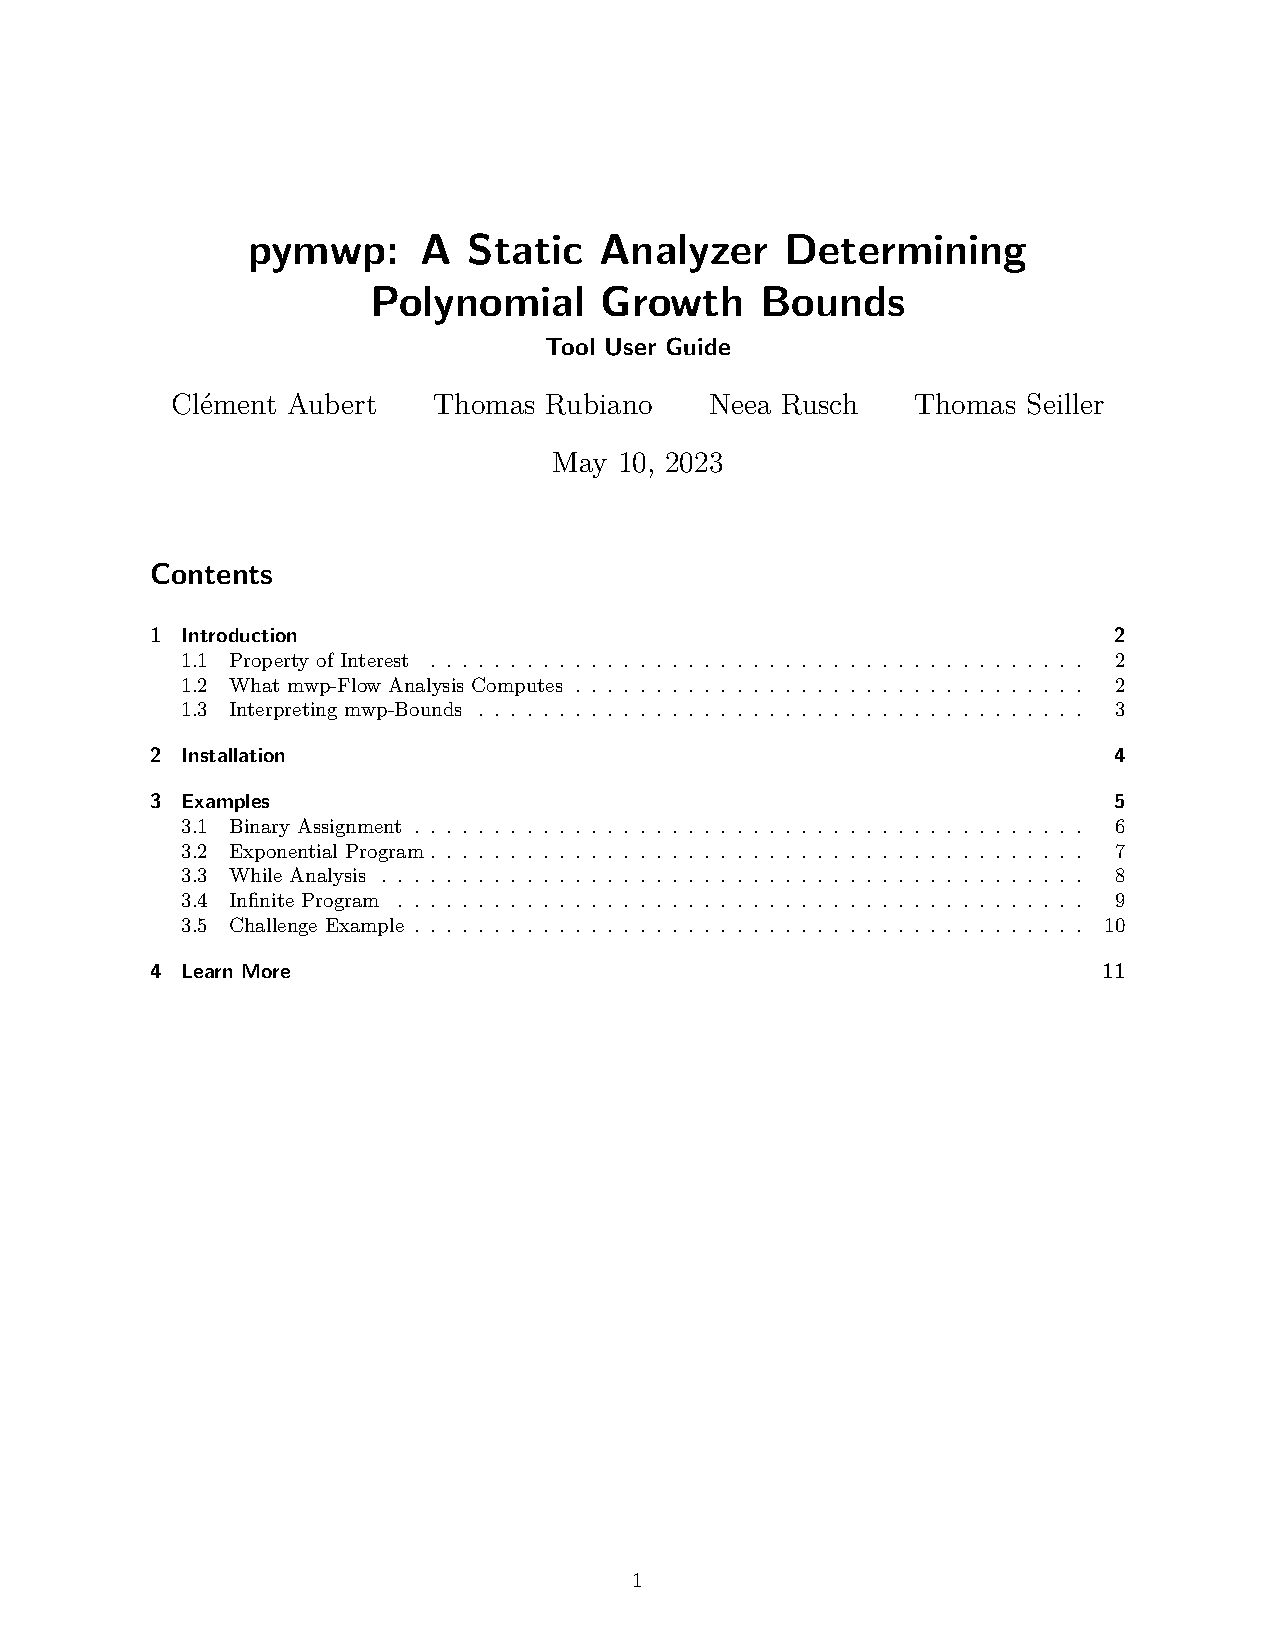
\includepdf[pages={1-},pagecommand={\thispagestyle{empty}\stepcounter{insertpages}
\ifnum\value{insertpages}=1\addcontentsline{toc}{section}{
Tool User Guide for pymwp: A Static Analyzer Determining Polynomial Growth Bounds}\fi
}]{res/pubs_pymwp_guide.pdf}\setcounter{insertpages}{0}

\end{document}